 %Please make sure you use the cover page available on Moodle. This template does not generate a cover page. 

\documentclass[11pt, twoside]{report}
\usepackage[utf8]{inputenc}
\usepackage{graphicx}
\usepackage{wrapfig}
\usepackage[a4paper, width=150mm, top=25mm, bottom=30mm, bindingoffset=20mm]{geometry}
\usepackage[toc,page]{appendix}
\usepackage{pdfpages}
\usepackage{natbib}
\usepackage{dirtytalk}
\usepackage{pdflscape}
\usepackage{longtable}
\usepackage{multirow}
\usepackage{textcomp}
\usepackage{fancyhdr}
\usepackage{tikz}
\usepackage{helvet}
\usepackage{hyphenat}
\usepackage{listings}
\usepackage{xcolor}
\renewcommand{\familydefault}{\sfdefault}
\def\checkmark{\tikz\fill[scale=0.4](0,.35) -- (.25,0) -- (1,.7) -- (.25,.15) -- cycle;} 
\pagestyle{fancy}
\fancyhf{}
\fancyhead[LE, RO]{\thepage}
\fancyhead[LO, RE]{\leftmark}
\setlength{\headheight}{13.6pt}
\linespread{1}
\bibliographystyle{Harvard}
\bibpunct{(}{)}{,}{a}{}{ }
\graphicspath{ {images/}{appendices/} }
\footskip = 15mm

\definecolor{codegreen}{rgb}{0,0.6,0}
\definecolor{codegray}{rgb}{0.5,0.5,0.5}
\definecolor{codepurple}{rgb}{0.58,0,0.82}
\definecolor{backcolour}{rgb}{0.95,0.95,0.92}

\lstdefinestyle{mystyle}{
    backgroundcolor=\color{backcolour},   
    commentstyle=\color{codegreen},
    keywordstyle=\color{magenta},
    numberstyle=\tiny\color{codegray},
    stringstyle=\color{codepurple},
    basicstyle=\ttfamily\footnotesize,
    breakatwhitespace=false,         
    breaklines=true,                 
    captionpos=b,                    
    keepspaces=true,                 
    numbers=left,                    
    numbersep=5pt,                  
    showspaces=false,                
    showstringspaces=false,
    showtabs=false,                  
    tabsize=2
}

\lstset{style=mystyle}

\begin{document}


\includepdf[pages=-]{docs/cover.pdf}

\chapter*{Abstract}
\textit{Aphanizomenon flos-aquae} is a filamentous cyanobacteria that inhabits fresh water. Cyanobacteria can produce toxins which degrade water quality, are dangerous to the health of both humans and aquatic animals, and incur a significant economic impact. Counting the number of cyanobacteria cells in a water sample provides a significant measure of its quality. Presently, this kind of cell counting task is usually performed by eye by expert microbiologists. Overlapping cells, variations in shape and size, and the subtle differences between species make this challenging. In addition, different human counters often count inconsistently, and the task is tedious and time-consuming.\\

In this project, a novel artefact is produced as part of an automatic counting solution for filamentous cyanobacteria cells. This artefact's central component is a neural network model, trained on a novel dataset of images depicting \textit{A. flos-aquae}. This artefact, and the experimental process by which it is developed, demonstrates that a neural network model for detection and localisation can be successfully applied to the task of cell counting. It also demonstrates how this approach might be improved upon in future work, chiefly by creating a richer dataset, using different base models for fine-tuning, and training for longer.

\chapter*{Acknowledgements}
I owe special thanks to my project supervisor Dr Pamela Johnston for her support, detailed feedback, and good humour; Adrian Brown of Fennex Ltd. for his patient guidance; and Alistair Kevan for helping me find the way through.

\tableofcontents

\listoffigures

\cleardoublepage
\pagenumbering{arabic}

%!TEX root = ../main.tex
% What is the project about? 
% What problem are you tackling? 
% What is your research question? 
% Why do these problems need solutions? Why are they important?
% What is the background to the problem? Who is the client? What do they want?
% What existing methods have been tried? How has I.T. been applied so far? 
% What constraints do you have? (Time, PCs, money, users, software etc) 
% What is the scope of what you have set yourself to do. What is not included?
% What broad approach was taken? (Summarise your broad approach the project) 
%%

\chapter{1. Introduction}
\label{chap:intro}
For humans, object counting in images can be an extremely time-consuming, menial, and difficult task. This is true of any domain, and with advances in machine learning, automatic counters have been applied to a variety of use cases, such as crowd surveillance (\cite{Zhang_2016_CVPR}), traffic monitoring (\cite{Zhang_2017_ICCV}), and microscopy cell counting (\cite{Identification-and-enumeration-of-cyanobacteria,xie2018microscopy}).\\

In microbiology, cells are usually identified and counted manually using optical microscopy (\cite{Identification-and-enumeration-of-cyanobacteria}). Microscope images can contain hundreds or thousands of cells which can overlap, vary in shape and size, and possess subtle morphological differences between species, making them a challenging counting task for humans. Human observers also inevitably raise issues with count subjectivity depending on their level of expertise. In a sample of trained personnel counting single-celled organisms in microscope images, \cite{Do-experts-make-mistakes} reported an observer count self-consistency rate of 67-83\% and a count consensus rate (\textit{between} observers) of only 43\%. Experts in making particular discriminations could be expected to achieve accuracies of 84 to 95\%.\\

The counting of cyanobacteria is a highly relevant application for an automatic counter. Cyanobacteria present a risk to the health of both humans and aquatic animals by producing toxins and degrading water quality. In turn they can incur significant economic losses due to the cost of water treatment and public healthcare (\cite{Identification-and-enumeration-of-cyanobacteria}). \cite{Do-experts-make-mistakes} showed that automatic counting methods can achieve human-level performance on cell counting tasks, and previous approaches by \cite{xie2018microscopy} and \cite{Identification-and-enumeration-of-cyanobacteria} have shown that cells (including those of cyanobacteria) can be counted using neural network-based approaches with reasonable accuracy. The aim of this project is to build upon existing work and develop a reliable, neural-network based approach to counting cyanobacteria cells, using a novel dataset of microscope images of the cyanobacteria \emph{Aphanizomenon flos-aquae}. Automatic cell counting is still relatively nascent and open to innovation, and a method to count filamentous cells such as those of \textit{A. flos-aquae} specifically would be novel.

%!TEX root = ../main.tex
%%

\chapter{Background}
\section{Datasets}
The data to be learned from is central to any machine learning task. Image datasets can range from hundreds to millions of instances, and can encompass any number of depicted classes from one to tens of thousands. Image data is usually subject to some form of preprocessing due to practical constraints: inputs to any neural network are required to be of fixed dimensionality and these dimensions cannot be excessively large (like high-resolution images). This usually leads to the resizing of images to fit as in \cite{Krizhevsky-2012}, where images were downsampled to 256x256 pixels, and \cite{LeCun-1998}, where the dataset was normalised to contain only 28x28-pixel images. \\

The dataset resulting from \cite{LeCun-1998}, MNIST, is ubiquitous in the field of machine learning. Containing 70,000 images, MNIST is small by comparison to modern datasets such as ImageNet, but its features (handwritten digits) are simple, and a modern network can be trained to near human-level performance on it (\cite{Krizhevsky-2012}). Contemporary datasets are orders of magnitude larger and contain far more complex features than older ones such as MNIST: ImageNet (\cite{imagenet_cvpr09_orig}) is a dataset of over 15 million high-resolution images depicting 22,000 distinct object categories. \\

The dataset used by this project (henceforth 'Micropics') is that used in the Micropics project\footnote{GitHub - pamelaajohnston/micropics. (no date). Available at: https://github.com/pamelaajohnston/micropics (Accessed: 19/11/2021)}. It comprises 311 microscope images of the cyanobacteria \textit{Aphanizomenon flos-aquae}. Each of the dataset's images has both an original and annotated version (where the ground truth of each cell's location in the image is annotated by a red dot). Compared to ImageNet, which contains a huge variety of raw and processed images taken by different cameras and with different styles, Micropics' images are taken under controlled conditions and are all highly similar. They also depict a single object class, the cells themselves. In the respect of being a relatively small and feature-limited dataset, Micropics is similar to the dataset used in \cite{xie2018microscopy}, which is a synthetic dataset created by \cite{Zisserman} (using the method described by \cite{Computational-framework}). This dataset comprises 200 images, and of these, random subsets of only 8 and 64 were used for training, with a further 100 for testing. The results of \cite{xie2018microscopy} from such a small dataset are promising for the few-shot learning that will be inevitable in this project due to the diminutive size of Micropics. The Micropics dataset is likely to be subject to a standard 70/30 or 80/20 split, but the effects of other splits could be explored.\\

\begin{figure}[h!]
	\centering
	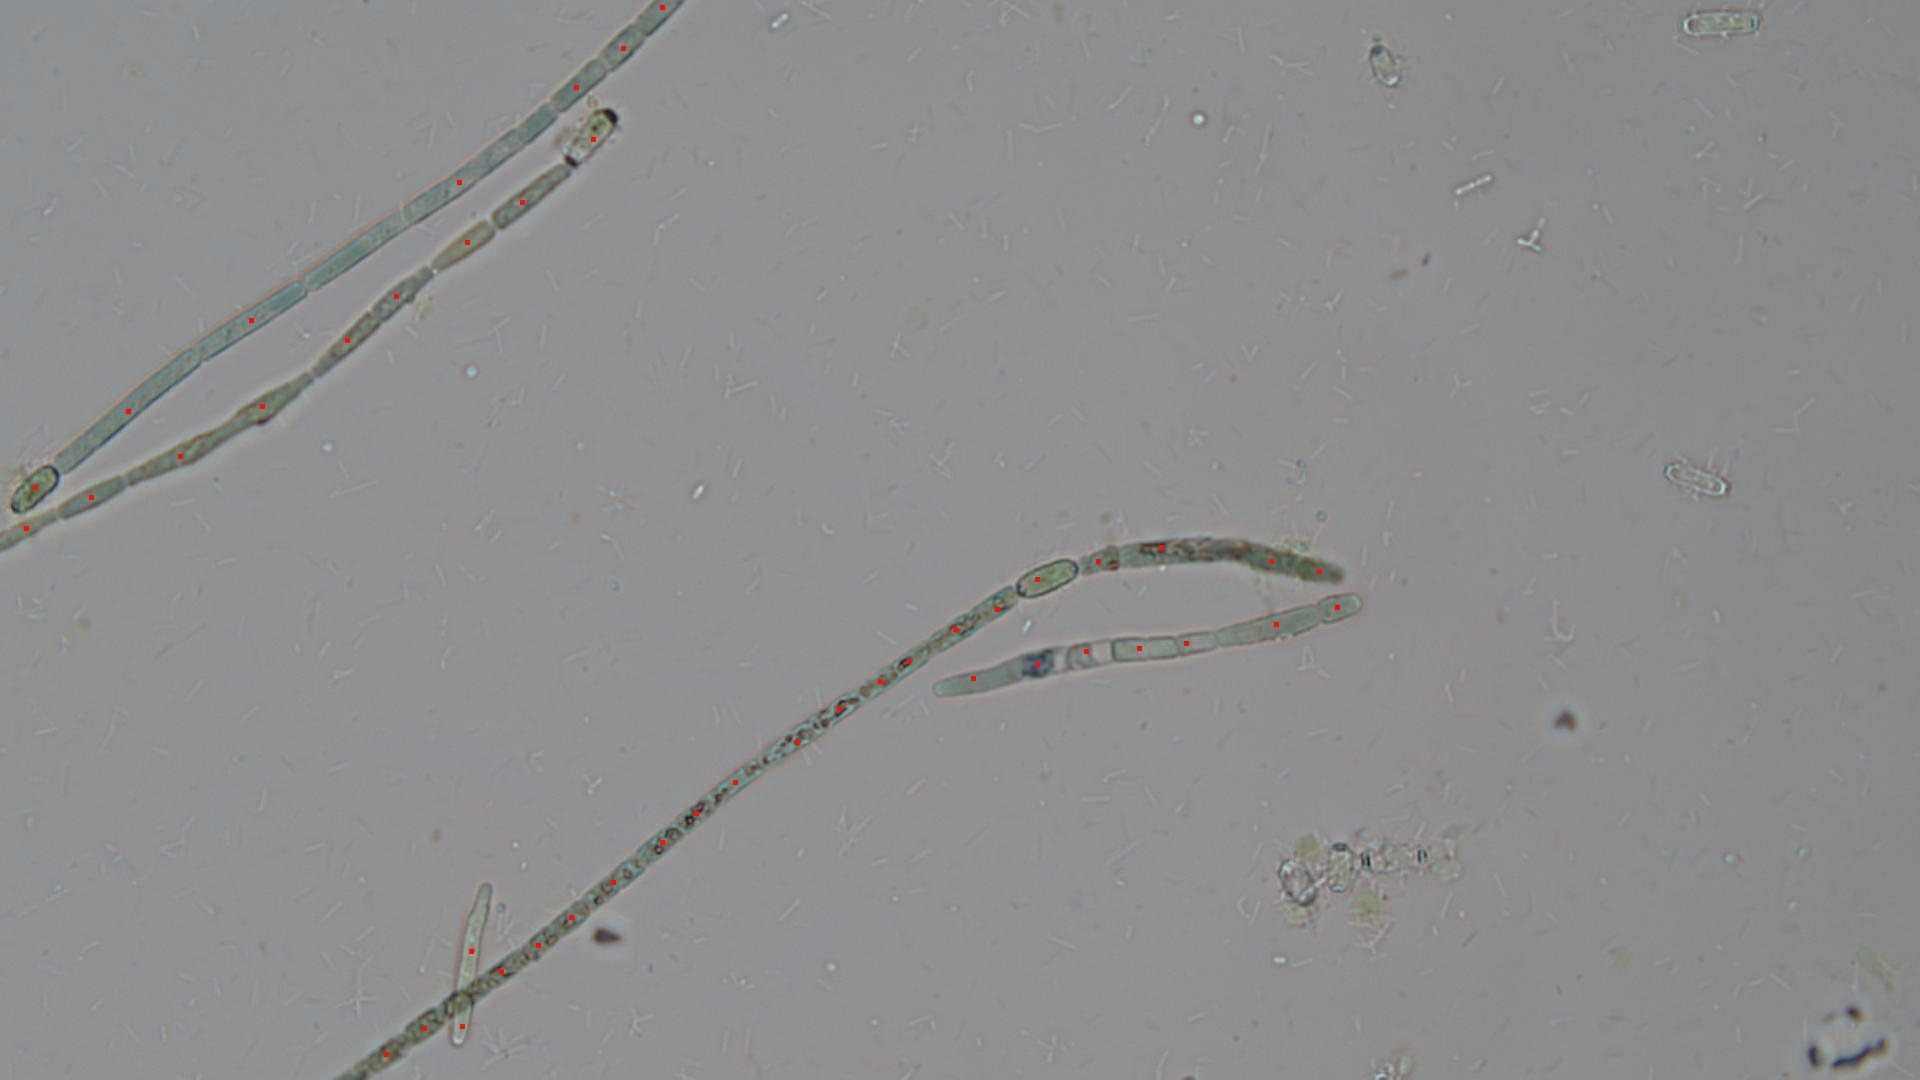
\includegraphics[width=0.5\textwidth]{images/02Background/micropics.jpg}
	\caption{An example of an annotated image from the Micropics dataset (red dots for ground truth)}
\end{figure}

In their unprocessed form, the images are unsuitable for learning due to their high resolution (1920x1080), so they must be either downsampled or converted to cropped patches. Downsampling an image necessarily causes information to be lost, and in the case of the images in Micropics, the objects to be counted are particularly small within the image, which is known to cause detection networks to fail (\cite{redmon2016look}); this problem would be exacerbated by downsampling. The ground-truth annotation dots (which are themselves part of the images) might also be blurred or made inconsistent by downsampling and antialiasing (which is a by-product of, for example, the downsampling method used in \cite{LeCun-1998}). Some networks such as YOLO (\cite{redmon2016look}) predict a limited number of objects per region of an image, and the images in Micropics depict close clusters of small objects, which YOLO is known to struggle with. Hence the decision to segment the images into size-normalised patches appears to be the best choice for the use case, an approach also taken by \cite{xie2018microscopy}.

\section{Convolutional Neural Networks}
The roots of the neural cell counting project are inseparable from those of neural networks themselves. These can be traced as far back as the first convolutional neural networks, which enabled the development of generalisable neural models for image recognition, localisation, and counting (\cite{LeCun-et-al-2015}).\\

The fully-connected neural network (NN) architecture is of limited use for processing images. These networks simply take an input image as a 1-dimensional vector of pixels, and propagate this through each fully-connected layer. This ignores the strong 2-dimensional structure of images, where pixels that are close together are strongly correlated, and local groups of pixel values can yield important patterns and features that are useful for identification. NNs also have no in-built tolerance for variations in position and size or distortions of features in images (\cite{LeCun-et-al-2015, LeCun-1998}). The development of Convolutional Neural Networks (CNNs) was motivated by the search for this region-invariant, feature-based detection, and inspired in part by the findings of \cite{hubel1962receptive}, who found that the visual cortex of cats was composed of ‘simple’ and ‘complex’ cells. Both types of cells detect edges and bar patterns with specific orientations, but while 'simple' cells detect these patterns only at specific locations, 'complex' cells are indifferent to the whereabouts of the pattern in the visual field. \cite{hubel1962receptive} proposed that 'complex' cells simply combined inputs from a number of 'simple' cells that detected the same pattern, but at different regions in the visual field, to produce their region-invariant properties. This concept that several 'simple' feature detectors can be summed to detect more 'complex' features is the underlying assumption of CNNs.\\

CNNs subject the input image to a process of ‘convolution’ which can extract the features of an image. A convolutional layer is a grid of neurons, the inputs to each of which are the units from a small neighborhood ('receptive field') in the previous layer (or the input image). Taking contextual inputs in this form allows the neuron to learn local features in an image. At the first convolution layers these features are simple edges and corners. Subsequent layers combine these simple features to learn higher-level ones. Since the neurons in a convolutional layer all share the same set of weights, they can detect features regardless of whether its location, size etc. in the input image changes (\cite{LeCun-1989}).\\

\begin{figure}[h!]
	\centering
	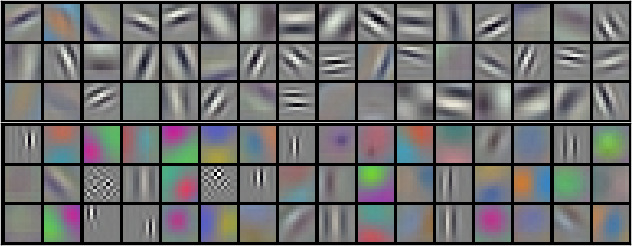
\includegraphics[width=0.5\textwidth]{images/02Background/filters.jpg}
	\caption{Features learned by the first convolutional layers of AlexNet (\cite{Krizhevsky-2012})}
\end{figure}

\cite{FUKUSHIMA1982455}'s Neocognitron was an early ancestor of the modern CNN which took direct inspiration from \cite{hubel1962receptive}. The Neocognitron was comprised of several modules, each containing a first layer of 'S-cells' connected to a second of 'C-cells'. These 'C-cells' achieved some success in digit recognition, but the Neocognitron relied upon an inferior, unsupervised reinforcement algorithm for training, since it was conceived before the development of the fully supervised backpropagation learning that would later enable remarkable achievements by CNNs.\\

Due to their proven track record (\cite{Krizhevsky-2012,girshick2014rich,redmon2016look}), CNNs are the network architecture of choice for reliable object detection in images (\cite{LeCun-et-al-2015}). CNNs are also broadly applied to automated counting applications, including the counting of cells; \cite{xie2018microscopy} and \cite{Identification-and-enumeration-of-cyanobacteria} both use CNN-based approaches to counting cells, even where cells are not individually detected, as in the case of \cite{xie2018microscopy}. Being the predominant method for object recognition and counting, there is a wealth of CNN-based image recognition and counting literature and software to learn from and build upon in the development of a new cell counter, making it the natural choice for further investigation.

\section{Detection}
Before cells can be counted, they must be detected. CNNs have been applied with great success to generalised object detection, and their feature-based learning holds promise for the task of detecting and counting cells.\\

\subsection{LeNet}
What became LeNet-5 was in development for nearly 10 years from 1989 to 1998. \cite{LeCun-1989} pioneered the first multi-layered CNNs and applied them to the task of image recognition, in LeNet’s case handwritten character recognition. By 1999 LeNet-5 was reading 10\% of all cheques in the U.S. (\cite{LeCun-et-al-2015}). \cite{LeCun-1989} makes reference to Fukushima’s Neocognitron, from which it takes inspiration for the network's convolutional architecture, but emphasises LeNet’s fully supervised learning using backpropagation and stochastic gradient descent, which freed LeNet from the highly problematic and difficult manual preprocessing that characterised previous attempts at feature extraction (\cite{LeCun-1989,8016501}). Using backpropagation, LeNet could learn the required features automatically.

\subsection{AlexNet}
After the early successes of LeNet, the use of CNNs stagnated through the 2000s, but the ImageNet 2012 competition could be credited with kick-starting the contemporary renaissance of interest in image recognition using CNNs (\cite{LeCun-et-al-2015}). On the ImageNet LSVRC-2010 dataset—a set of 1.2 million images together depicting 1000 distinct object classes—AlexNet, the model described in \cite{Krizhevsky-2012}, achieved a ‘top-1 error rate’ of 37.5\% (where the most confident class predicted by the model is incorrect), and a ‘top-5 error rate’ (where the correct class is not present in the model’s top 5 predictions) of 17.0\%. These scores defined the state of the art at the time, and AlexNet went on to win the LSVRC-2012 competition with a top-5 error rate of 15.3\%, more than 10\% less than the second-place model.\\

This unprecedented performance can be attributed to several innovations in AlexNet. At the time of this achievement the \textit{de rigeur} neural activation functions for hidden units in a network were the hyperbolic tangent \(f(x) = tanh(x)\) and logistic sigmoid \(f(x)=\sigma(x)\) \cite[p. 191]{Goodfellow-et-al-2016}). LeNet as an example used \(tanh\) as its activation or ‘squashing’ function. AlexNet conceived of applying the Rectified Linear function \(f(x)=max(0,x)\) to this purpose, creating a network of Rectified Linear Units (ReLUs). This circumvents two key weaknesses suffered by \(tanh\) and sigmoid. The first is that the \(tanh\) and sigmoid functions are relatively computationally intensive compared to the exceedingly simple ReLU. With a dataset as large as ImageNet this results in a severe upper limit on the size of a network that could be trained on the data, due to excessively high training times. ReLU also allowed the network to avoid the second weakness suffered by \(tanh\) and sigmoid, the well-documented ‘Vanishing Gradient’ problem (\cite{Dying-ReLU}), where at high or low input values, the gradient of tanh and sigmoid is close to zero and provides little to no useful information to influence the model during backpropagation. This innovation allowed AlexNet to train on ImageNet 6 times faster than an equivalent network using \(tanh\) units, enabling it to train to an exceptionally high accuracy. It also made use of a regularisation technique known as 'Dropout', new at the time, which randomly and temporarily deactivates a proportion of the units in the network when training on a new image. This ensures that units do not become reliant on the presence of other units, and a unit must therefore learn features that are useful with \textit{any} configuration of the other neurons in the network. This method makes AlexNet resilient against overfitting.\\

The legacy of AlexNet is broad and deep. The use of the once-ubiquitous \(tanh\) and sigmoid activation functions is now discouraged \cite[p. 191]{Goodfellow-et-al-2016}, and ReLU (and its derivatives such as LeakyReLU) has become a default choice for modern neural networks. While AlexNet is now an antiquated network, it laid the groundwork for many successors (\cite{redmon2016look}'s YOLO uses both a ReLU-derived activation function and Dropout) which have been applied to all manner of tasks, not only object detection but also object localisation and counting.

% At high or low input values, the gradient of both functions is close to zero and provides little to no useful information to influence the model during backpropagation when the function is derived. ReLU’s linearity above 0 means it never ‘saturates’ at higher values, i.e., its gradient does not level off. The ‘non-saturating’ property attributed to the neurons in AlexNet is in reference to this, and it means the units do not suffer from vanishing gradients at higher values during learning.

% \cite{Krizhevsky-2012} omits to mention that ReLU \textit{does} inherently suffer from the vanishing gradient problem at values below zero: since the gradient below zero is zero, if ReLUs are subjected to negative inputs they may fall into a state where they only output zero for any input and cannot be recovered, becoming ‘dead’ and of no use to the network. This is a well-understood issue known as the ‘Dying ReLU’ problem (\cite{Dying-ReLU}). The dying ReLU problem has since been addressed in various ways, including various hand-designed and generated functions intended to supersede it, but as noted by \cite{Searching-for-Activation-Functions}, the plethora of functions proposed to supersede ReLU show inconsistent performance across different tasks and datasets. Many also introduce further complexity to the process of training the network in the form of an extra parameter to be tuned. Nonetheless, the use of the once-ubiquitous tanh and sigmoid activation functions is now discouraged \cite[p. 191]{Goodfellow-et-al-2016} and while ReLU has become a 'default' choice for modern neural networks (\cite{Goodfellow-et-al-2016,Searching-for-Activation-Functions}), optimising activation functions remains an open question.

\section{Localisation}
Detecting cells is a prerequisite to \textit{localising} each cell in an image. The images in Micropics are annotated with this in mind: the location of each is denoted by a dot annotation. Once the location of all cells is known, counting is trivial. Several techniques exist for object localisation in images.

\subsection{R-CNN \& Derivatives}
R-CNN (\cite{girshick2014rich}) was introduced as an adaptation of the CNN for object localisation rather than classification. Given an input image, R-CNN generates around 2000 'region proposals' or 'regions' from the image (each itself an image), based on which areas are deemed likeliest to contain an object. In \cite{girshick2014rich} this is determined by the selective search algorithm, although there are many other algorithms for region proposal and the network is agnostic to the algorithm used. Each region proposal is category-independent, not referring to any particular object class. Subsequently, each region is resized and forward-propagated through a deep CNN (an implementation of AlexNet with no classification layer). This results in a 'feature vector' for each region proposal. Finally, each feature vector is classified using a Support Vector Machine and each region proposal assigned a confidence score, and the scored regions are distilled by discarding the lower scoring region where any two regions containing the same class are overlapping.\\

\begin{figure}[h!]
	\centering
	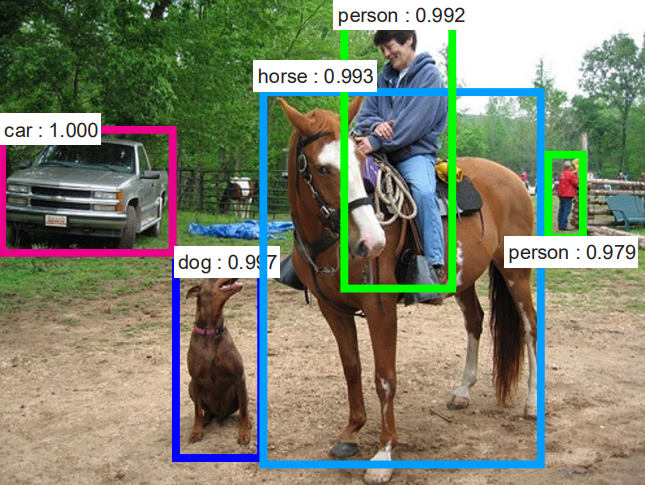
\includegraphics[width=0.5\textwidth]{images/02Background/rcnn.png}
	\caption{An image processed by Faster R-CNN (\cite{ren2016faster})}
\end{figure}

One disadvantage of the R-CNN system is that it is relatively slow. In \cite{girshick2015fast}, an R-CNN network was found to take 47 seconds to process a single image at test time. This led to the development of Fast R-CNN (\cite{girshick2015fast}), and Faster R-CNN (\cite{ren2016faster}). The former of these achieved 213 times faster test-time processing than R-CNN and higher detection quality. The latter achieved a processing speed of 6 images per second, approaching real-time performance. R-CNN and its derivatives have seen successful applications to the detection of pedestrians (\cite{Fast-CNN-Pedestrians}), faces (\cite{Fast-R-CNN-Faces}), and the counting of cells (\cite{Identification-and-enumeration-of-cyanobacteria}), and a PyTorch-based implementation of Faster R-CNN is available as part of Detectron 2, Facebook AI's object-detection library\footnote{GitHub - facebookresearch/detectron2. (no date). Available at: https://github.com/facebookresearch/detectron2 (Accessed: 19/11/2021).}. Detectron is open-source and development is highly active, making Faster R-CNN a reliable option for a counting project.

\subsection{YOLO}
Following Faster R-CNN, another object-localisation network was developed, realising Faster R-CNN's aspirations for real-time performance: \cite{redmon2016look}'s YOLO. YOLO has the advantage over Faster R-CNN of consisting of only a single component for both detection and localisation, compared with Faster R-CNN's relatively complex pipeline. Compared to the state of the art at the time (R-CNN and derivatives), YOLOv1 made more errors in localising objects, but predicted fewer false positives and maintained a competitive mAP (mean average precision). It also showed a greater ability to generalise than Faster R-CNN. Most crucially, it was capable of processing images at 45 frames per second. YOLO has since been updated several times, and in the task described by \cite{benjdira2018car}, it was shown that YOLOv3 exhibited not only dramatically faster, but also better performance than Faster-CNN.\\

YOLO's remarkable speed makes it more suitable than other networks for experimentation using commercial hardware. The original author (\cite{redmon2016look}) developed YOLO to version 3, but an open-source PyTorch version known as YOLOv5 is currently maintained by Ultralytics\footnote{GitHub - ultralytics/yolov5. (no date). Available at: https://github.com/ultralytics/yolov5 (Accessed: 19/11/2021).}. This is a highly active project, and would serve as a reliable basis for experimentation in applying the YOLO network to the domain of cell counting. Alternatively, an implementation of YOLOv3 is available for Keras \footnote{GitHub - qqwweee/keras-yolo3. (no date). Available at: https://github.com/qqwweee/keras-yolo3 (Accessed: 19/11/2021).}.

% AlexNet popularised the use of ReLUs, but YOLO takes this a step further by using a network of LeakyReLUs. LeakyReLU is linear for inputs above zero, but for inputs below zero returns the input multiplied by a (small) value \(\alpha\), creating a small gradient. LeakyReLUs always return some gradient, which mitigates the ‘Dying ReLU’ problem caused by ReLU’s vanishing gradient below zero. However as previously noted in \cite{Searching-for-Activation-Functions}, ReLU-derived functions such as LeakyReLU do not reliably generalise to all tasks and there is scope to explore the effects of the activation function as an additional network parameter.

\section{Counting} \label{density-estimation}
If a network can detect and localise cells in an image, counting the cells becomes trivial (\cite{Zisserman}). However, direct detection of individual objects is not the only method available for counting, and another method known as 'density estimation' has also been applied to the domain of cell counting.

\subsection{Detection vs. Density Estimation}
R-CNN and other detection-based methods have been shown to produce reliable counts from images; \cite{Identification-and-enumeration-of-cyanobacteria} uses it to localise and count cyanobacteria cells. While detection-based counting can be highly effective, the efficacy of object detection tends to degrade when objects are occluded or overlapping (\cite{Zisserman}). An alternative method of obtaining a count of objects is to estimate their density in an image. This is done by learning a \textit{mapping} between the global features of an image and a count of the objects depicted by it. This is the approach taken by \cite{xie2018microscopy}. Both \cite{Zisserman}  and \cite{xie2018microscopy} use images whose ground truth is provided by by dot annotations at the locations of objects (as in the Micropics dataset). The system then learns a density map from the features of the image that is trained to match the ground truth as closely as possible.\\

\begin{figure}[h!]
	\centering
	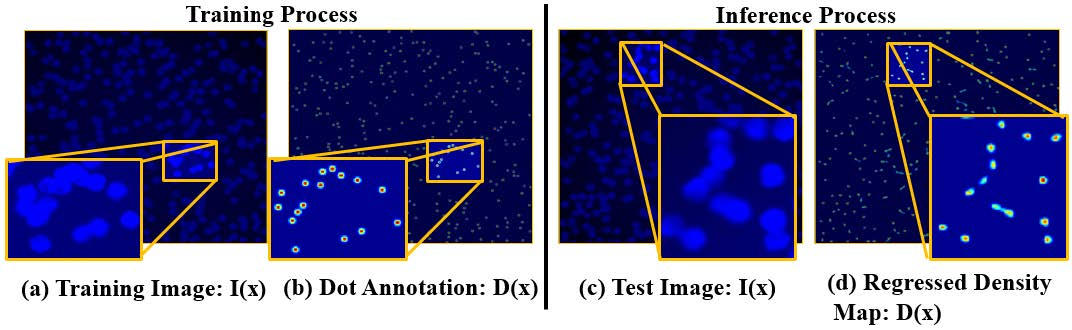
\includegraphics[width=0.5\textwidth]{images/02Background/density.jpg}
	\caption{An example of a learned density map (\cite{xie2018microscopy})}
\end{figure}

Existing density estimation-based counting methods, while achieving success in cell counting, have so far been tested on images (synthetic or otherwise) of cells which are non-filamentous; the structure of filamentous bacteria such as \textit{A. flos-aquae} is quite different, and it is unclear how a density estimation-based approach would transfer to the task of counting filamentous cyanobacteria. \cite{Liu_2018_CVPR} points out that while the density-estimation method is effective for densely crowded images where detection-based methods struggle, density-estimation approaches equally tend to \textit{over}estimate where the density of objects in an image is sparser. This is certainly the case in Micropics, where the filamentous cells are arranged in long lines, rather than clusters, against an empty background. The viability of density estimation-based counting for filamentous cells remains an open question, and a possible alternative to a detection-based method using YOLO.

\section{Conclusion}
As specified at the outset, the objective of this project is to develop an automatic cell counter for filamentous cyanobacteria. There is sufficient scope to find improvements upon current methodology, since the investigation of current literature revealed questions and avenues for further development. The best model to implement for the purpose of the project appears to be YOLO, which has been demonstrated to be a state-of-the-art CNN for image recognition that is also extremely fast compared to other networks. Being so lightweight, it is feasible that YOLO could run at test time on commercial hardware, but given the potential for repeated training it may be necessary to make use of a GPU provided by the University to train the network. Both PyTorch and Keras options are available, but the PyTorch implementation, being more up-to-date, is the more likely candidate. In the event that a detection-based approach with YOLO similar to \cite{Identification-and-enumeration-of-cyanobacteria} is revealed to be unfeasible, the viability of using a density-estimation approach as in \cite{xie2018microscopy} and \cite{Zisserman} on filamentous bacteria could be further investigated.

\subsection{Evaluation}
The cell counter will be a software artefact with a well-defined goal, making it relatively easy to evaluate. The counter should be capable of accepting unannotated images of \textit{A. flos-aquae} from Micropics and returning a number representing a reliable count of cells in the image. The counter's loss can be defined as the absolute distance between this predicted count and the count of ground-truth dot annotations in the annotated image (which can be retrieved by a Python script present in the Micropics repository). This error can be evaluated against that of existing approaches. Another evaluation metric for the model could be to determine the quality of its predicted bounding boxes versus the ground-truth bounding boxes, by their Intersection Over Union (IOU) (defined as the number of pixels that were correctly predicted divided by the number encompassed by both bounding boxes). However, the error in cell count is the only metric strictly needed to evaluate the artefact.\\

The network loss on both training and test sets should be monitored. Since the dataset is small, splitting it into only test and train sets may be desirable rather than also including a validation set. This introduces the problem that while tuning hyperparameters, the network may overfit on both test and train sets while appearing to improve (\cite{zhang2017understanding}). Ideally the network should be tested on an additional validation set to ensure it is not overfitting. An alternative is to use K-fold cross-validation to ensure the network learns from all examples in the dataset. When the model's loss plateaus, it is likely that it is unable to learn any more information with its current hyperparameters, and some tuning will be required. The network hyperparameters are all the more important given the diminutive size of Micropics, since a smaller latent space means there is greater likelihood of falling into a local minimum. Tuning of hyperparameters such as the batch size, number of epochs, and learning rate (or varying the learning rate over training, to prevent the network from oscillating) would be useful for further evaluation of different network configurations, but in a trained network such as YOLO, the selection of hyperparameters available for tuning is likely to be limited.

%!TEX root = ../main.tex
%%

\chapter{Design \& Methodology}
Neural network models (specifically CNNs) have previously shown efficacy in cell recognition and counting, so a model of this kind will be the core component of the cell counting artefact. The artefact will process input images and return a reliable count of cells in the image as an output.\\

The project will be evaluated on the following requirements, which are prioritised according to the MoSCoW method. ‘Must’ requirements are essential to the project’s success, and the project’s success will be evaluated on them. ‘Should’ requirements add value to the project beyond its core functionality, but are not essential. ‘Could’ requirements add further value but are the lowest-prioritised, and their implementation should not be attempted unless all higher-priority requirements are implemented and time remains for development.

\section{Requirements}
\subsection{Functional Requirements}
\subsubsection{Must}
\paragraph{As an input, accept an image (or image patch) from the dataset.}
At the least, the artefact should accept input images from the Micropics dataset, or patches thereof. The images in the dataset have a resolution of 1920x1080, so are not usable in a neural network model in their unprocessed form. Some neural networks, like YOLO, accept images of an arbitrary shape and size, but will still subject these images to transformation (e.g. cropping or padding with zeros) in order that they can be processed. These transformations could negatively affect the model’s performance, particularly since the objects to be counted are small. To solve this problem, the images could be segmented into smaller patches that can be processed by the model.

\paragraph{As an output, produce a reliable count of cells in the image.}
This requirement can be evaluated using the ground-truth images in Micropics. The Micropics project includes a script to return a count of the ground-truth dots in an image, so the artefact can be evaluated by the mean absolute error of the artefact’s guesses versus the ground-truth numbers.

\paragraph{Process any valid input without errors}

\subsubsection{Should}
\paragraph{Use the optimal hyperparameters for the model.}
The artefact can only achieve its highest possible performance by using the optimal set of model hyperparameters. This will require extensive testing and trial and error.

\subsubsection{Could}
\paragraph{Produce a secondary output for explanation purposes.}
In anticipation that the user desires (or is entitled to) an explanation of the output of the artefact, it could be designed in such a way as to produce one. This would likely take the form of a copy of the input image with any cells highlighted.

\paragraph{Include a user interface.}
The working artefact in its simplest form is not usable by the layman, but a UI could be developed to make it more useful for lay users.

\subsection{Non-functional Requirements}
\subsubsection{Must}
\paragraph{Use Python for development.}
Python is the default language for machine learning tasks.  Many Python libraries exist for image classification use cases, as well as implementations of neural network models YOLO and Faster R-CNN.

\paragraph{Be trained and tested on the Micropics dataset.}
The Micropics dataset defines the project goal, to count filamentous cyanobacteria cells in images. The dataset may be subject to additional processing, or annotation depending on the model used: for example, the only form of ground truth that YOLOv5 accepts is bounding box annotations around each object to be classified.

\paragraph{Have a corresponding project log.}
This is a requirement of any Honours Project, and will provide a valuable record of the evolution of the project.

\paragraph{Use a capable machine for computation.}
Access to a suitable GPU can be sought from Google Colaboratory or the University.

\paragraph{Be completed by the End of Year Show date.}

\subsubsection{Should}
\paragraph{Use a deep CNN model for detection-based counting of cells (such as Faster R-CNN or YOLO).}
Deep CNN models have previously shown success in the task of detection-based enumeration of cells in images, and implementations of such detection-based models are readily available.

\paragraph{Process an input image quickly at test time.}
Image processing speed is dependent on the model used, but modern localisation networks such as YOLO and Faster R-CNN process images in a trivial amount of time. Processing should not be expected to take more than 1 minute.

\paragraph{Process training data quickly at train time.}
Training time is dependent on the complexity of the model and the training pipeline, so the optimal training parameters (epoch number, batch size etc.) should be found through experimentation. Training time is also dependent on the size of the dataset, so a subset could be used instead of the full dataset. In this case a tradeoff would have to be considered between the size of the dataset used and the model’s performance, since the model will improve with more data.

\paragraph{Be backed up to a version control system.}
To prevent data loss, the project must exist redundantly on a remote repository (likely GitHub).

\paragraph{Be functional by the due date of the Proof of Concept deliverable.}

\subsubsection{Could} 
\paragraph{Use the Pytorch implementation of YOLOv5.}

\paragraph{Use the Keras implementation of YOLOv3 or v4.}

\paragraph{Use Faster R-CNN.}

\subsubsection{Use a density estimation method to count cells.}
Density estimation, rather than detection-based counting, has recently emerged as an alternative method for object counting. This could be explored for comparison with a detection-based method.

\section{Methodology}
\subsection{Legal, Social \& Ethical Issues}
The Micropics dataset is internal to the University and contains no sensitive data, so its use does not present any ethical concerns. In the first instance, the artefact serves as a proof of concept, and is not meant to be used for any safety-critical cell counting application.\\

Inevitably, some count error will be present, but the artefact should ideally err on the side of overcounting rather than undercounting, since false positives are more desirable than false negatives in this case. False negatives might lead to severe consequences for human and animal health, for example if a contaminated water source was determined to be safe, whereas a false positive might inconsequentially be reviewed by a human operator.

\subsection{Data Preparation}
To allow the images in Micropics to be used in training and testing of a neural network, while preventing the destruction of any information in the images by cropping or scaling, the full-resolution images will be split into patches using the \verb|patchRGB.py| utility from the Micropics repository\footnote{GitHub - pamelaajohnston/micropics. (no date). Available at: https://github.com/pamelaajohnston/micropics (Accessed: 05 May 2022).}. Of the 311 images in the Micropics dataset, 20 images each from both the dot-annotated set and the unannotated set will be used. 20 full images was seen as a suitable number for the project because, when split into 224x224 pixel patches, they amount to an acceptably large dataset size of 640 patches while also minimising time spent on the time-consuming and menial annotation process. This allows for a good tradeoff between annotation and experimentation. The patches will be segregated into train, test, and validation sets. Initially the train/test/validation split will be 50/25/25, allowing for experimentation to determine the effect of adding more training data.

\subsection{Data Annotation}
The existing data annotation in Micropics takes the form of a red dot drawn at the centre of each cell. This annotation is incompatible with any detection model including YOLO, so the dataset must be reannotated. The only form of annotation YOLO will accept is edge-aligned rectangular bounding boxes, encompassing each instance of the object(s) to be detected. Several software tools exist for the purpose of annotating images in this way.

\subsubsection{Label Studio}
Label Studio\footnote{Label Studio – Open Source Data Labeling. (no date). Available at: https://labelstud.io/ (Accessed: 21 Apr 2022)} is an open-source data annotation tool widely used in industry. It offers the option to export annotations to many formats, including YOLO. In addition to images, many other types of data can be annotated, including audio and text. Keyboard shortcuts are included for navigation through the dataset, and are based around the WASD configuration, freeing the mouse hand for drawing.\\

Two issues were apparent with Label Studio for the purposes of this project. The one first noticed involved its web-based user interface. During annotation, images are displayed on the page at their actual size and cannot be enlarged. 'Zooming' into the image is possible, but only results in the zoomed image remaining cropped within a box the size of the original image. Since the image patches are 224-pixel squares, they are particularly small on a high-resolution display and this makes annotation difficult (see Figure \ref{label-studio-large}).\\

\begin{figure}[h!]
	\centering
	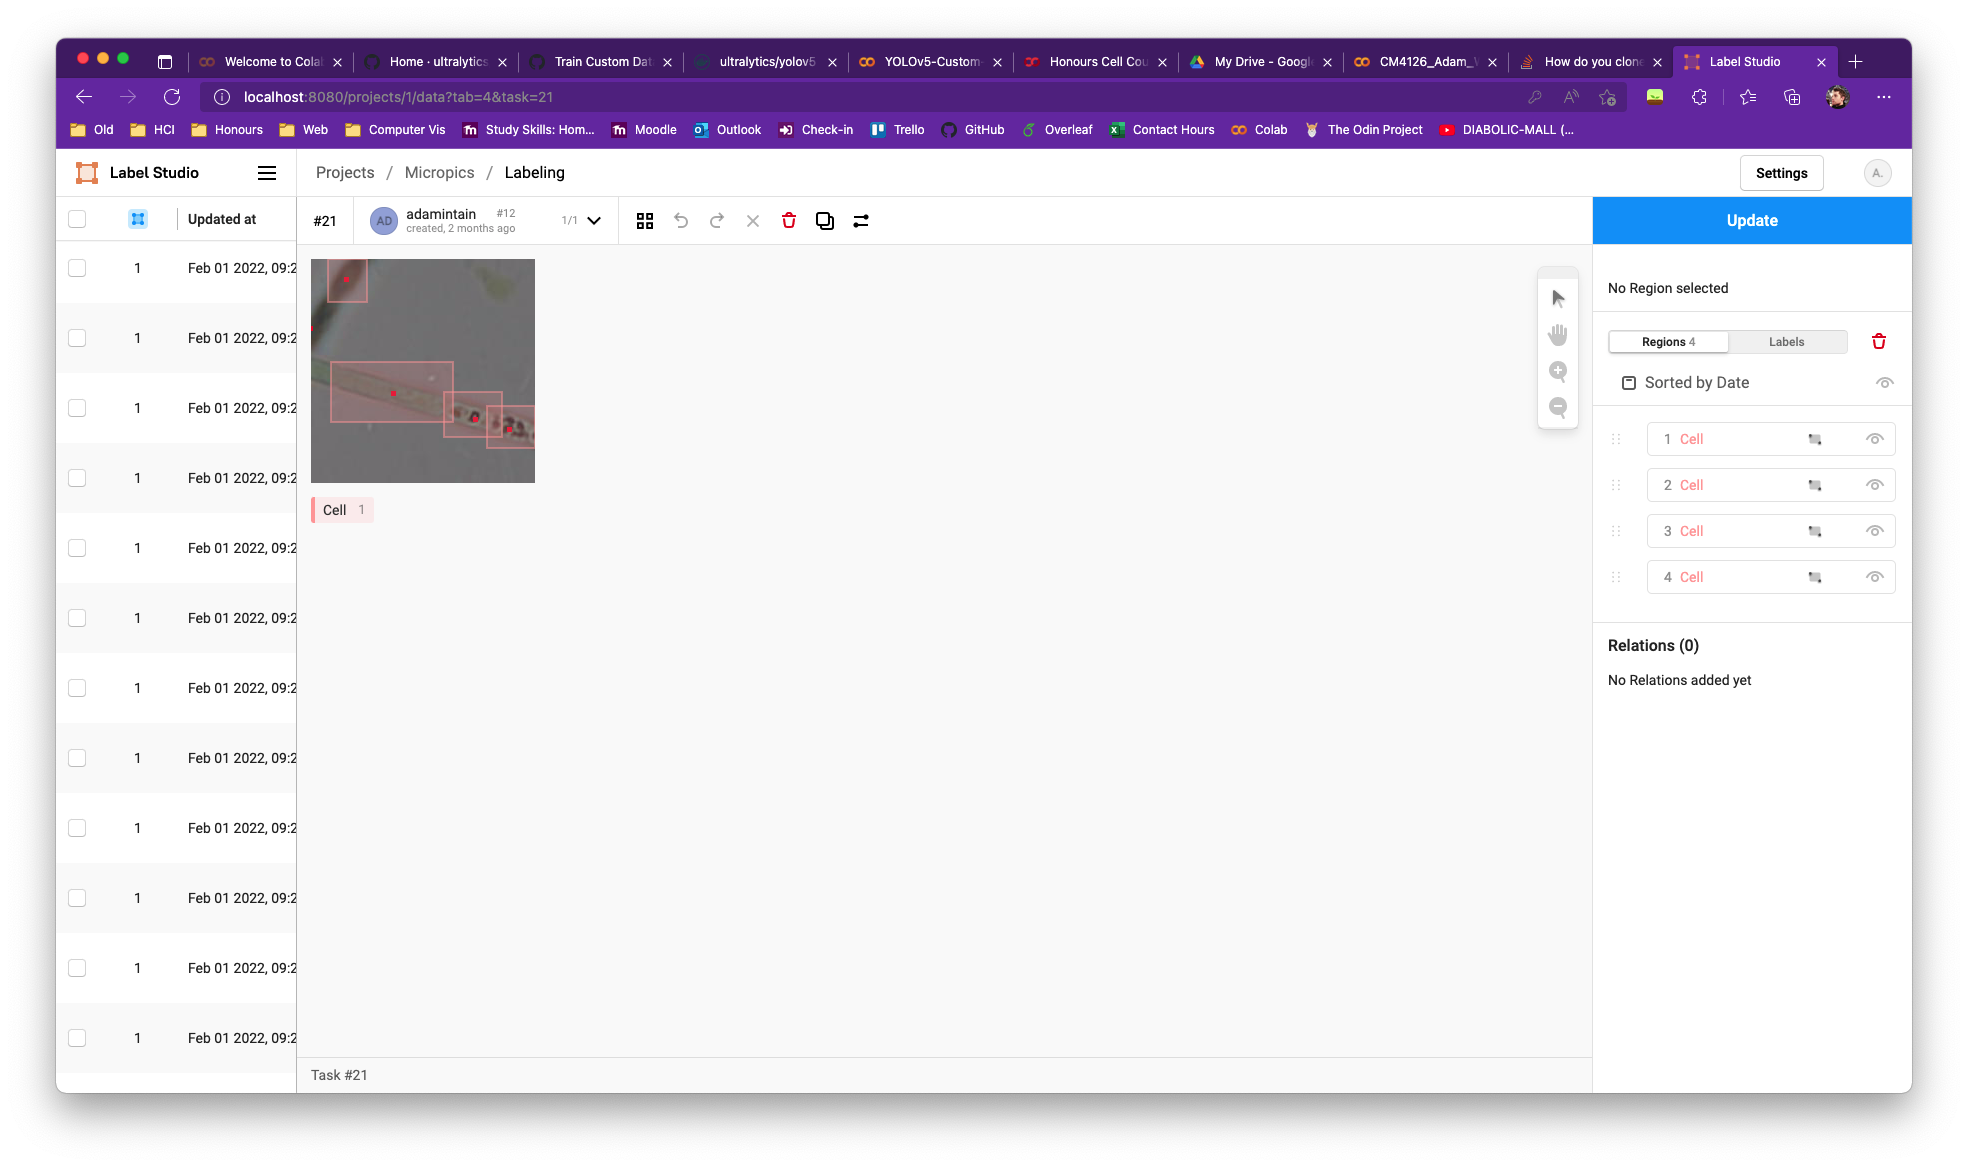
\includegraphics[width=0.8\textwidth]{images/03Design/label-studio-large.png}
	\caption{Label Studio's user interface on a high-resolution display}
    \label{label-studio-large}
\end{figure}

The second feature of Label Studio that made it less suitable for this project was the fact that a sequence of random characters is prepended to the filename of each exported image and label (see Figure \ref{label-studio-prefix}). In this project, the dot-annotated images from the dataset are used for annotation, but the unannotated originals are used in training. The mismatch between image and label filenames means that exported labels cannot be used with the unannotated images without a solution to remove these filename prefixes.

\begin{figure}[h!]
	\centering
	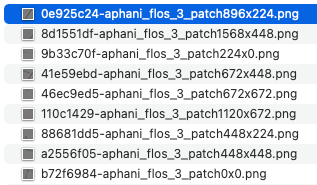
\includegraphics[width=0.5\textwidth]{images/03Design/label-studio-prefix.png}
	\caption{Images annotated by Label Studio with random filename prefixes}
    \label{label-studio-prefix}
\end{figure}

\subsubsection{LabelImg}
LabelImg (see Figure \ref{labelImg}) is another open-source image labeller which exports YOLO-format annotations\footnote{GitHub - tzutalin/labelImg. (no date). Available at https://github.com/tzutalin/labelImg (Accessed: 21 Apr 2022).}. It is an older, better-established tool than Label Studio, with more than double the number of GitHub 'Stars' (17.2k to 8.1k). It is also strictly limited to image annotation.\\

LabelImg was found to be a highly ergonomic tool for navigating and annotating the dataset, which did not suffer from either of the aforementioned issues with Label Studio. In LabelImg, the image being annotated simply grows or reduces with the window size, allowing small images to be 'zoomed' on large displays. Filenames for label files always match the filename of the corresponding image, eliminating the problem of filename mismatch between labels and unannotated images. Some options had to be configured⁠—'Use Default Class Label' and 'Auto Save Mode' were toggled on to prevent object class and save prompts from appearing when drawing a bounding box or moving to a new image⁠⁠—but once these steps were taken, navigating the dataset and drawing bounding boxes was easy, and was streamlined by the presence of WASD-based keyboard shortcuts for dataset navigation, as in Label Studio.

\begin{figure}[h!]
	\centering
	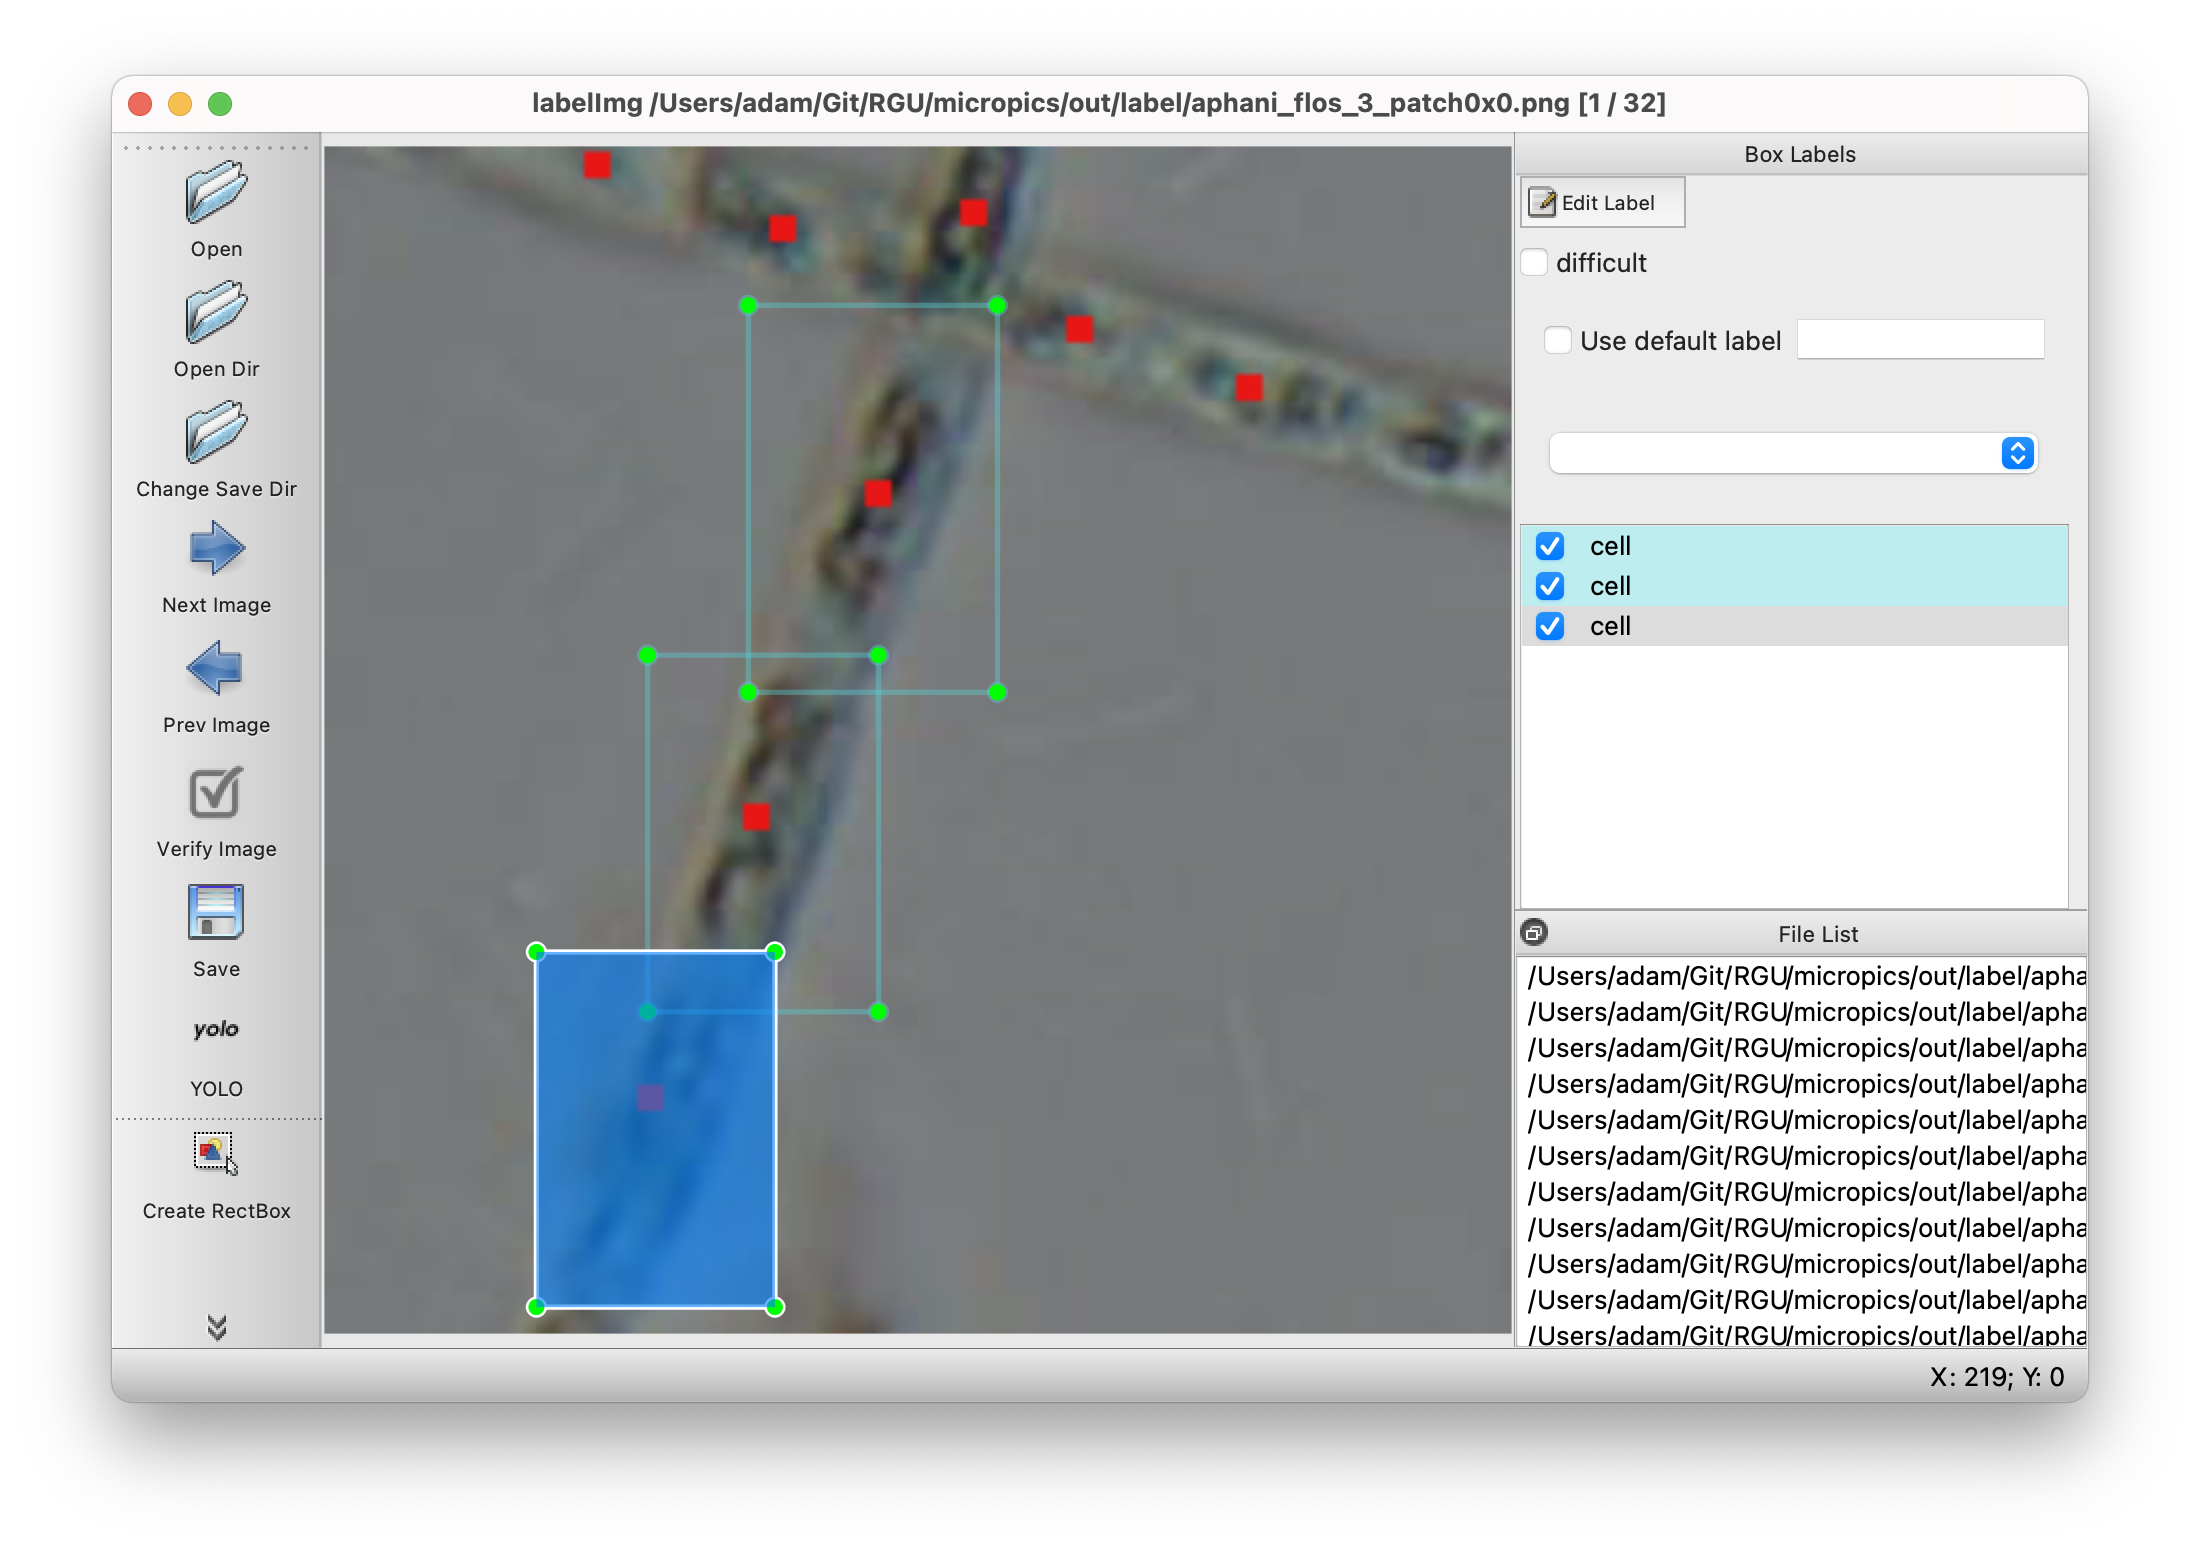
\includegraphics[width=0.8\textwidth]{images/03Design/labelImg.png}
	\caption{LabelImg's user interface}
    \label{labelImg}
\end{figure}

\subsubsection{Annotation Rules}
Annotation presents a particularly significant challenge in the project's methodology. The lack of domain knowledge on the part of the annotator means that even in the dot-annotated images, it is often difficult to distinguish cells in the same trichome from each other. Wherever this significantly affects annotation, it will be taken into account that annotation dots are located at the centre of each cell, and bounding boxes will be drawn around this central dot so as to slightly intersect the bounding boxes on either side.\\

Other cells are difficult to label because they are dot-annotated but out-of-focus, occluded by other cells, or exceeding the edge of the patch. Some ground rules for labelling are required to avoid ambiguity. For the first version of the annotations, in order to be labelled, it will be required that cells are:

\begin{enumerate}
    \item Dot-annotated
    \item In focus
    \item Unoccluded
    \item Wholly visible and not appearing to exceed the edge of the patch
\end{enumerate}

\subsubsection{YOLO Annotation Format}
A dataset in YOLO is defined by a YAML file (e.g. \verb`data.yaml`), which contains the base path to the dataset and the directories of each subset (train, test, validation) relative to this base path (an example can be seen in Listing \ref{yaml}). This file must be created manually, and the dataset must be organised as specified in the file. During training, YOLO will use the YAML file to automatically find corresponding labels for images by looking in the \verb|<database-path>/labels| directory, but filenames for labels must be identical to those of the corresponding images. The YAML file is passed as the \verb|--data| argument when training is run.\\

Label files are in \verb|.txt| format, and list each instance of a labelled object in their corresponding image (an example can be seen in Listing \ref{label}). Each instance comprises the object class, the coordinates of the bounding box centre, and the bounding box's width and height. In addition, a \verb|classes.txt| file, specifying any object classes labelled in the dataset, must reside in any directory containing annotation files. This file is automatically generated by LabelImg.

\begin{lstlisting}[caption={YAML file for the project dataset}, label={yaml}]
path: /content/drive/MyDrive/dataset
train: images/train
val:  images/val
test: images/test

# number of classes
nc: 1

# class names
names: ["cell"]
\end{lstlisting}

\begin{lstlisting}[caption={An image annotation file in YOLO format. From left to right: object class; coordinates of bounding box centre; bounding box width and height}, label={label}]
0 0.781250 0.200893 0.241071 0.187500
0 0.462054 0.285714 0.227679 0.339286
0 0.368304 0.564732 0.218750 0.290179
0 0.267857 0.821429 0.241071 0.312500
\end{lstlisting}

% \begin{figure}[h!]
% 	\centering
% 	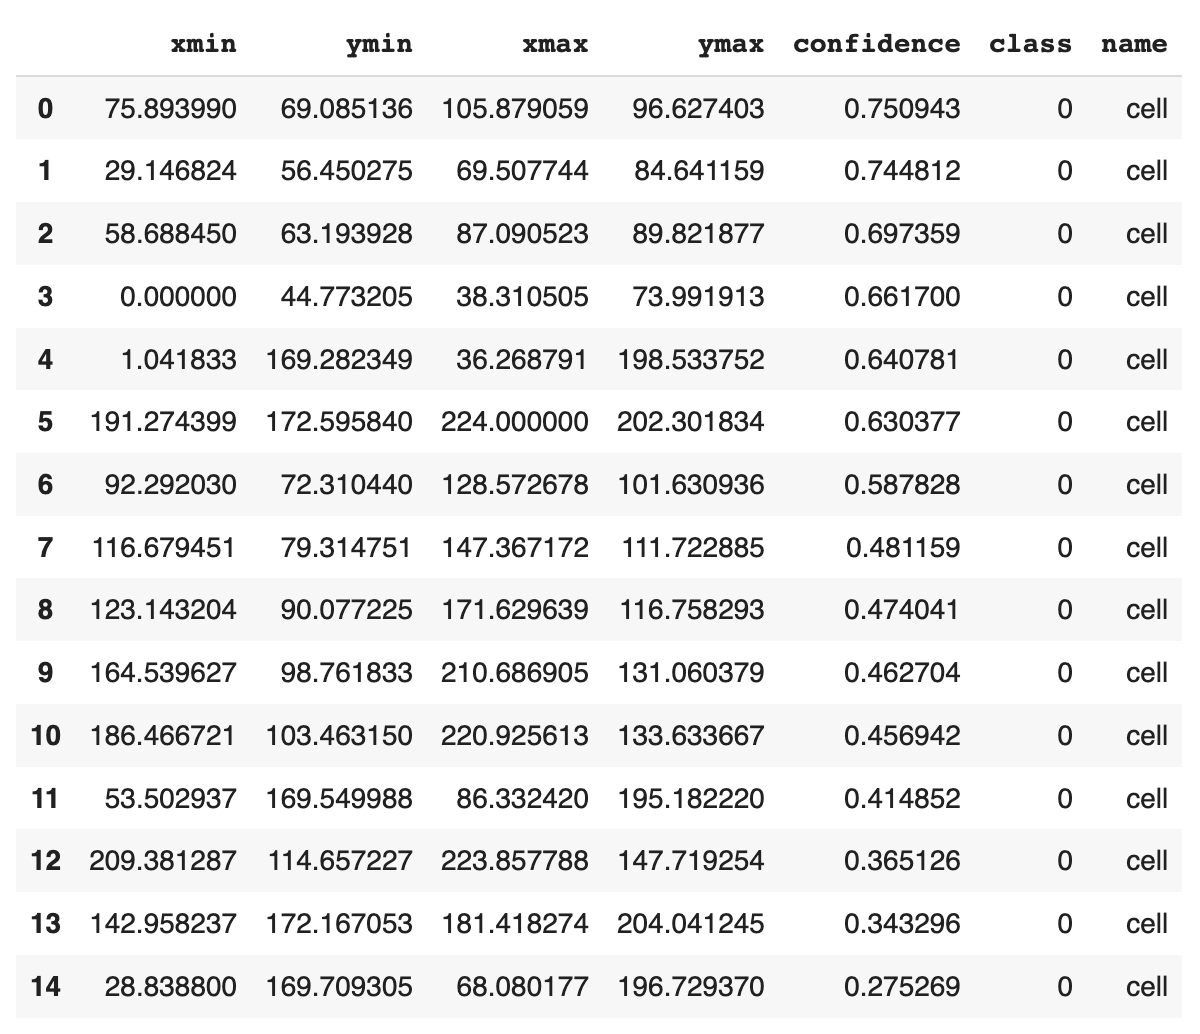
\includegraphics[width=0.8\textwidth]{images/04Implementation/dataframe.png}
% 	\caption{Custom YOLOv5 model's predictions on an image patch from Micropics (DataFrame)}
% \end{figure}

\subsection{YOLO Model}
Many implementations of YOLO exist for both Keras and PyTorch. Some of these are implemented by the community at large, such as a popular implementation of YOLOv3 for Keras\footnote{GitHub - qqwweee/keras-yolo3. (no date). Available at https://github.com/qqwweee/keras-yolo3. (Accessed 22/04/2022).}. Community-developed implementations of YOLO are less reliable than a primary source, since they are maintained by unpaid volunteers and, especially in the case of older YOLO versions, are vulnerable to abandonment. The repository for the aforementioned Keras implementation was last updated on 31 July 2018, and has 477 open issues at the time of writing. Documentation for the repository is also scarce.\\

Ultralytics are the present developers of YOLO in its latest incarnation, YOLOv5. They are the primary source for YOLOv5, which is implemented in PyTorch, and also offer an implementation of YOLOv3 in PyTorch which is in active development. Both of these implementations are offered in their respective GitHub repositories \footnote{GitHub - ultralytics/yolov3. (no date). Available at: https://github.com/ultralytics/yolov3 (Accessed: 05/05/2022).} \footnote{GitHub - ultralytics/yolov5. (no date). Avaliable at https://github.com/ultralytics/yolov5 (Accessed: 05/05/2022).}, and both include a wiki with extensive documentation and tutorials on the network. Compared to a community-maintained YOLO, these qualities of Ultralytics' YOLOv5 make it the better choice as a basis for experimentation.\\

Several pretrained models of varying levels of complexity (see Figure \ref{model_comparison}) are provided with YOLOv5, from YOLOv5n (least complex) to YOLOv5x (most complex), but no pretrained model is suitable for the cell counting use case (see Figure \ref{broc} and Table \ref{yolov5s_counts}), so a custom model must be produced by fine-tuning a pretrained model using the project dataset. Any of the pretrained models can be used as a basis for fine-tuning, so the effects of using different pretrained models can be appraised. The model chosen for initial experimentation was YOLOv5s. Being the second-smallest network, it allows for exceptionally high training speeds, which is ideal for the testing of different combinations of hyperparameters, annotations, and train/test splits. Later experiments might investigate the effects of using a larger and more complex base model. The fact that YOLOv5s is relatively lightweight may also have implications for this use case: the cell counter artefact might be deployed in deprived or rural areas with limited access to clean water, and where human experts are unavailable. In this case it might be deployed on less capable hardware with little or poor networking, and a less complex, more portable model would be desirable in this case.

\begin{figure}[h!]
	\centering
	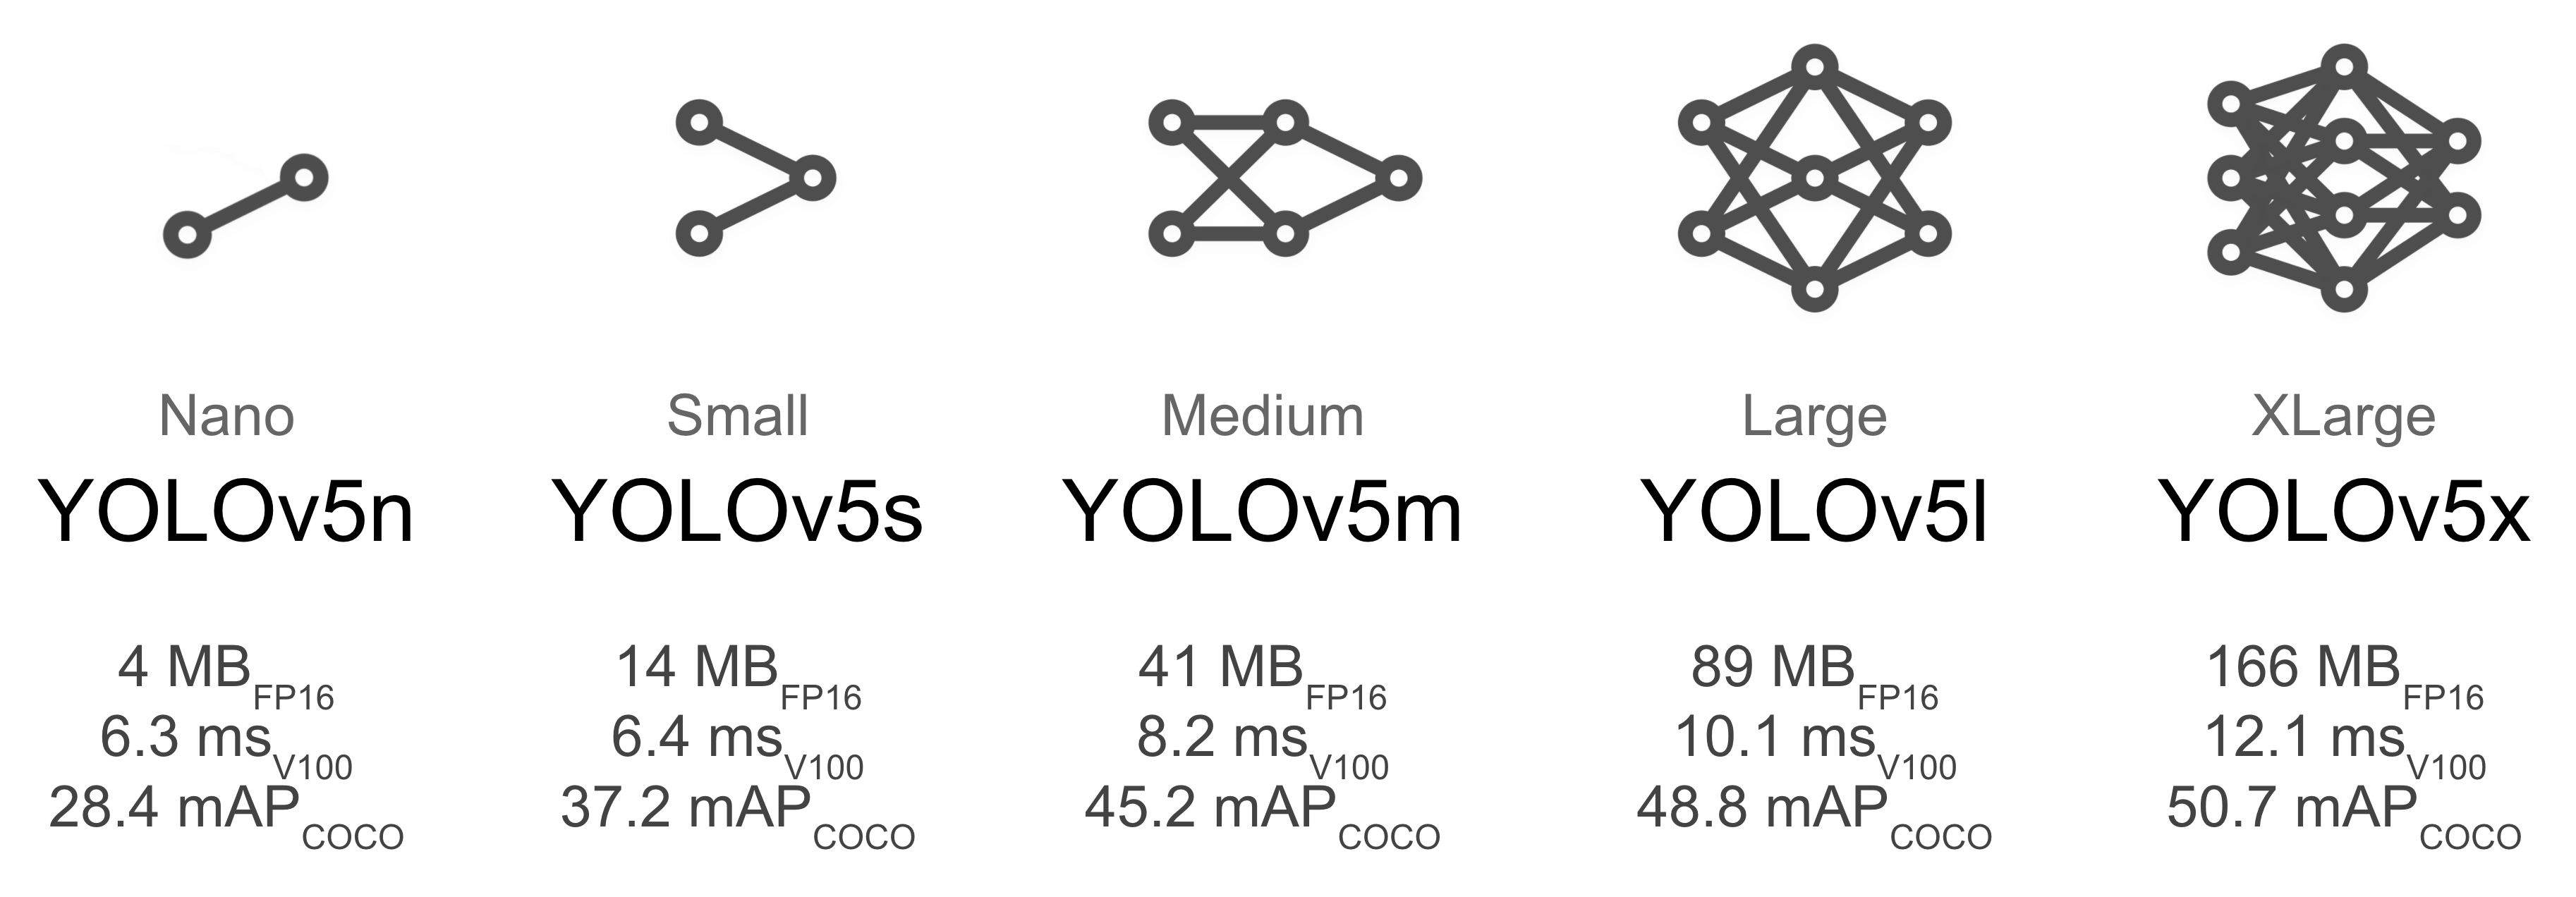
\includegraphics[width=0.8\textwidth]{images/04Implementation/model_comparison.png}
	\caption{Pretrained YOLOv5 models}
    \label{model_comparison}
\end{figure}

\begin{figure}[h!]
	\centering
	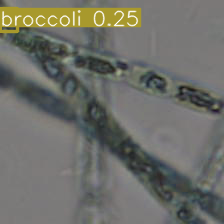
\includegraphics[width=0.5\textwidth]{images/03Design/broc.png}
	\caption{Bounding box predictions on a patch from the test set using YOLOv5s}
    \label{broc}
\end{figure}

\begin{table}
\centering
\begin{tabular}{ |l||l|l|l|l|  }
\hline
\multicolumn{5}{|c|}{Count Error} \\
\hline
Image & Ground Truth & Model Count & Num. Error & Pct. Error \\
\hline
37 &            81 &            1 &          80 &   98.765432 \\
39 &            58 &            3 &          55 &   94.827586 \\
41 &            86 &            0 &          86 &  100.000000 \\
44 &           102 &            0 &         102 &  100.000000 \\
\hline
\end{tabular}
\caption{Count error using YOLOv5s}
\label{yolov5s_counts}
\end{table}

% \begin{table}[h!]
% \centering
% \begin{tabular}{||c c c c c||} 
% \hline
% Image &  Ground Truth &  Model Count &  Num. Error &    \% Error \\
% \hline\hline
% 37 &            81 &            1 &          80 &   98.765432 \\
% 39 &            58 &            3 &          55 &   94.827586 \\
% 41 &            86 &            0 &          86 &  100.000000 \\
% 44 &           102 &            0 &         102 &  100.000000 \\
% \hline
% \end{tabular}
% \caption{Predictions on test set images from Micropics using YOLOv5s (counts)}
% \label{table:1}
% \end{table}

\subsection{Computation Platform}
While YOLOv5 is a fast network, it would be optimal for experiments to be run on a specialised platform for computation-heavy tasks. Multiple runs of training with varying hyperparameters can be dramatically accelerated by GPU computation.

\subsubsection{University DGX}
The first option for computation appraised was the University's Nvidia DGX server. This would provide high throughput and require no monetary investment, so was seen as a desirable option. Upon further investigation, it was found that setting up the DGX to serve a Jupyter Notebook for computation was difficult, and seemed to be obstructed by issues with the machine. Some time was spent identifying the issue before it was tentatively pinpointed as another user appropriating all GPUs. In addition, the outdated CUDA library present on the machine meant that the latest Tensorflow and Jupyter versions could not be installed, resulting in a reliance on older code. At this point the DGX-based approach was abandoned.

\subsubsection{Google Colaboratory}
Google Colaboratory (Colab)s\footnote{Colaboratory. (no date). Available at https://colab.research.google.com (Accessed: 22/04/2022).} provides free and premium access to GPU computation and a Jupyter Notebook environment. Notebooks are stored in the cloud via Google Drive and accessed through a web-based user interface. Google Drive integration also allows datasets to be stored in the cloud along with notebooks, providing a safe storage solution to prevent loss of either code or data during experimentation. Colab offered a harmonious and exceptionally easy-to-use alternative to setting up a computation environment from scratch, where all elements would need to be configured separately and connected.\\

Colab provides a free tier of access to GPU computation, but this is limited and liable to run out during long tasks. A Colab Pro subscription (£8.10 per month) provides more lenient access to computation. Based on its ease of use, web-based nature, and integration with cloud storage, it was decided that Colab represented the best option for the project's computation environment.

\subsection{Evaluation}
The artefact can be straightforwardly evaluated by its counting error, but this should take into account that a consistently overcounting artefact is more desirable than an undercounting one. YOLOv5 also produces various metrics for the model's detection and localisation performance, and these should also be evaluated.\\

For evaluation purposes, it is essential to keep a record of model performance—preferably with detailed results and metrics for each experiment—and to keep the resulting models backed up. Due to the volatile nature of a Colab runtime, any result of a YOLO training experiment, including the model, will be lost when the runtime is disconnected. Measures should be taken to prevent this. YOLOv5 features integration with 'MLOps' platform Weights and Biases\footnote{Weights & Biases – Developer tools for ML. (no date). Available at: https://wandb.ai/site (Accessed: 05/05/2022).}. Once logged in, W\&B automatically detects YOLOv5 training runs, keeps track of all metrics, and saves them to the cloud along with the resulting model. This replaces the otherwise burdensome and risky strategy of extracting models and metrics manually from the Colab runtime, so it was decided W\&B would be used for the purposes of this project. W\&B also presents this data in a user-friendly format (see Figure \ref{wandb}), generating graphs and images to explain otherwise opaque data about the model's performance.

\begin{figure}[h!]
	\centering
	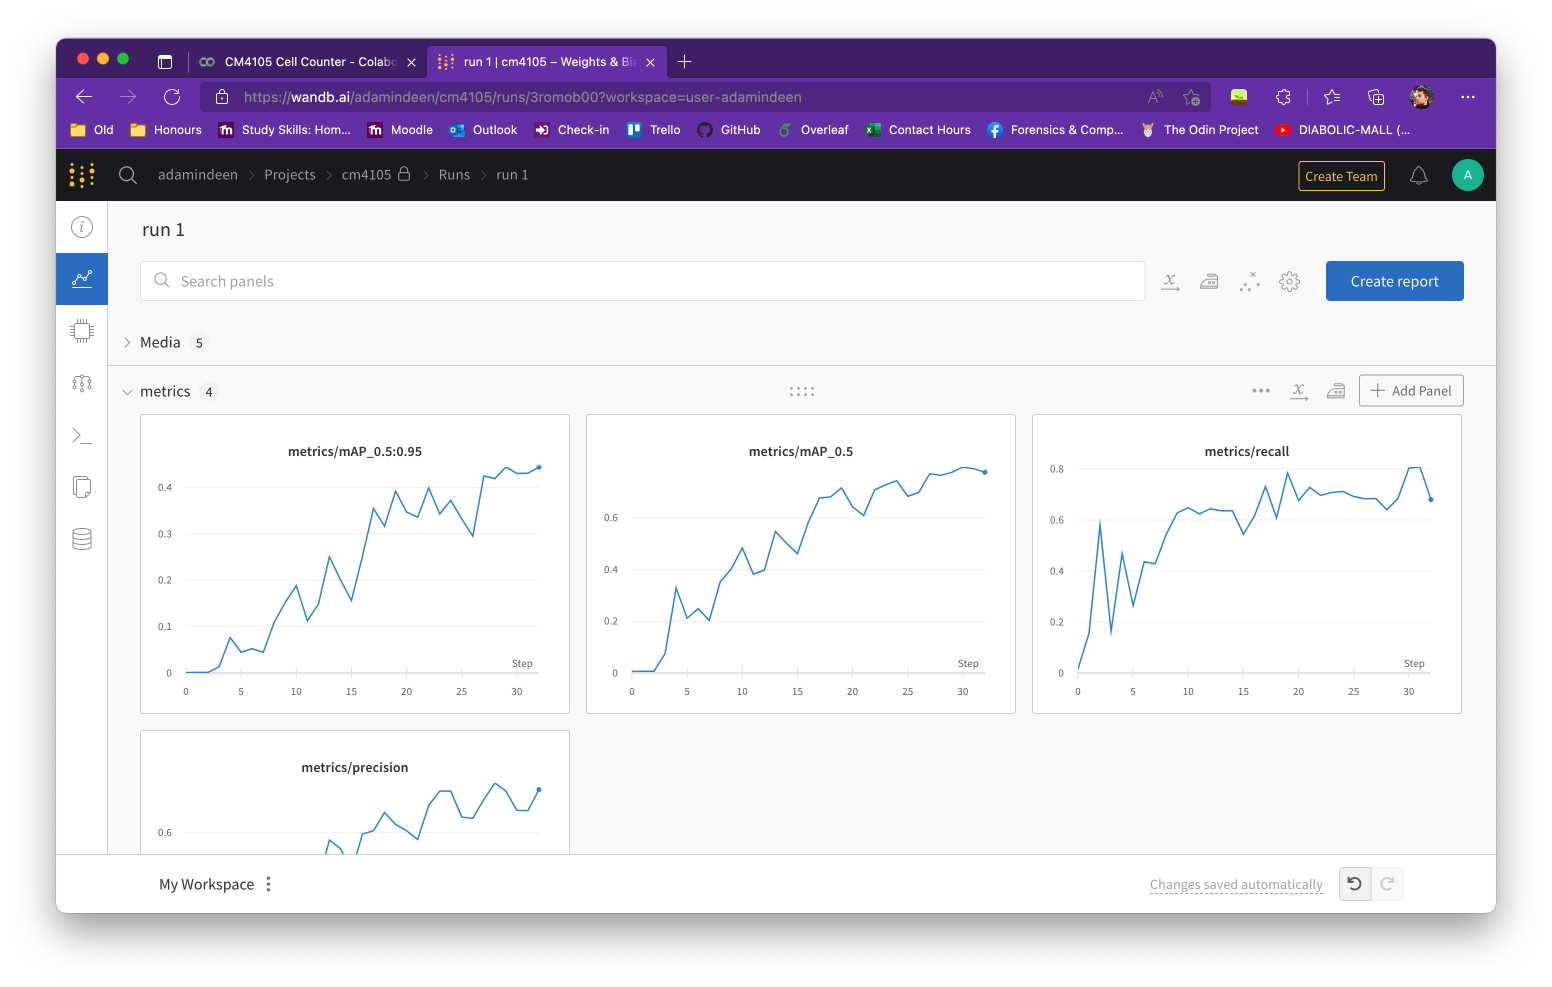
\includegraphics[width=0.8\textwidth]{images/03Design/wandb.png}
	\caption{Weights and Biases' user interface}
    \label{wandb}
\end{figure}

\label{chap:chapter3}



%!TEX root = ../main.tex
% %

\chapter{Implementation}

\section{Data Preparation}
Once the 20 images comprising the project dataset were split into patches, the dot-annotated set was reannotated using LabelImg. The unannotated patches were then split into train, test, and validation subdirectories in the \verb`/image` directory, and the label files produced from annotation were placed into the corresponding subdirectories in the \verb`/labels` directory (see Figure \ref{directories}). Since Google Colab was being used for computation, the dataset was uploaded to Google Drive to ensure it was easily accessible \& safely stored in the cloud.

\begin{figure}[h!]
	\centering
	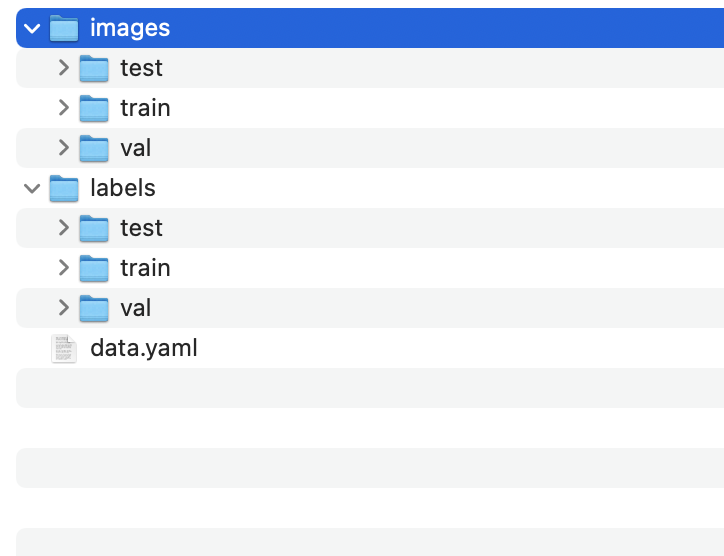
\includegraphics[width=0.5\textwidth]{images/04Implementation/directories.png}
	\caption{Directory structure for the project dataset}
	\label{directories}
\end{figure}

\subsection{Annotation}
The images in Micropics are sparse; cells appear in close groups rather than being evenly distributed. This means that many image patches could be skipped during annotation because they were were empty of cells. The final training set (70\% of the full dataset) comprised 384 images, but only 202 corresponding label files existed after annotation (Version 3), meaning that around 53\% of the training set was comprised of blank patches. The first version of the annotations took around 3 hours to complete.

\section{Training}
Prior to training, Weights and Biases was initialised to collect training statistics. 7 experiments were run; the configurations for each experiment are detailed in Table \ref{configs}.

\subsection{Annotation Revisions}
Disappointing initial results prompted the revision of the data annotations. The model appeared to fail to detect cells and undercounted significantly as a result, so it was decided that the criteria for labelling should be broadened to provide more information for the model to learn from. The annotations were subject to two revisions, both of which took substantially less time than the first attempt. In both revisions, the rules adhered to in the first version were modified:\\

\paragraph{Version 2} included cells which were dot-annotated and unoccluded, but out-of-focus \emph{or} exceeding the edge of the patch (but not both).\\

\paragraph{Version 3,} in addition to the cells included by Version 2's criteria, included those which were both out-of-focus \emph{and} exceeding the edge of the patch edge, and an attempt was made to include occluded cells where they could be told apart.\\
 
\subsection{Train/Test Split}
For the first and second experiments, 50\% of the dataset was reserved for training, with the other 50\% itself being split 50/50 into test and validation sets. After the 2nd run this 50/25/25 split was revised to 70/15/15 to explore the effect of a larger training set.\\

\subsection{Base Model}
In later experiments, the base model was changed from the lightweight and fast YOLOv5s to the more substantial YOLOv5l, an 89MB model with more than 40 million parameters which took more than twice as long to train as YOLOv5s.

\subsection{Epochs}
For the first experiment, a tentative 30 epochs was used to avoid overfitting. It was found in later experiments that increasing the number of epochs did not cause the model to overfit, even at 300 epochs, and that increasing the number of epochs had a pronounced effect on the model's counting capabilities.

\subsection{Batch Size}
Batch size started at 16 and was briefly kept at 32, on the recommendation of \cite{DBLP:journals/corr/abs-1804-07612} to use small batch sizes. However, later experiments instead heeded the recommendation of the YOLOv5 documentation\footnote{Tips for Best Training Results · ultralytics/yolov5 Wiki. (no date). Available at: https://github.com/ultralytics/yolov5/wiki/Tips-for-Best-Training-Results (Accessed: 05/05/2022).} to use substantially higher batch sizes, and this was increased to 128.

\begin{table}
\centering
\begin{tabular}{ |l||l|l|l|l|l|}
\hline
\multicolumn{6}{|c|}{Experiment Configurations} \\
\hline
Experiment & Annotations & Train/Test/Val Split & Batch Size & Epochs & Base Model\\
\hline
1 & v1 & 50/25/25 & 16 & 32 & YOLOv5s\\ 
 2 & v2 & 50/25/25 & 32 & 25 & YOLOv5s\\
 3 & v3 & 70/15/15 & 32 & 25 & YOLOv5s\\
 4 & v3 & 70/15/15 & 32 & 50 & YOLOv5s\\
 5 & v3 & 70/15/15 & 32 & 50 & YOLOv5l\\
 6 & v3 & 70/15/15 & 128 & 300 & YOLOv5s\\ 
 7 & v3 & 70/15/15 & 128 & 300 & YOLOv5l\\
\hline
\end{tabular}
\caption{Configurations for each run of training}
\label{configs}
\end{table}

\section{Counting}
Once the custom detection model is trained and⁠—in principle⁠—capable of detecting all cells in an input image, the detected cells can be counted easily, and the artifact's counting component was developed for this purpose. This component's principal function is \verb|count(directory, edge)|. This function uses YOLOv5's \verb|detect.py| script to run batch inference on all image patches in the \verb`directory` passed. Batch inference returns a \verb|Detections| object which contains a number of Pandas DataFrames, each of which corresponds to an image patch. Each DataFrame includes a row for every object detected in the patch; this allows for easy counting by looping through all the DataFrames, calling \verb|len()| on each to return a count of objects detected in the patch, and summing all patch counts. For the purposes of debugging and qualitative evaluation, \verb|count(...)| also prints the first DataFrame in the \verb|Detections| object, alongside the associated image patch with predicted bounding boxes.\\

It was recognised early on during testing that the model tended to count the same cells twice where they spanned 2 patches, and the fact that inference data was returned in the form of DataFrames allowed for a method to control for this. Since each row in the DataFrame includes the minimum and maximum extents of each predicted bounding box, a condition was included in \verb|count(...)| to simply discard any object with a bounding box that intersects with the top-left edge of the patch (by default, within 2 pixels of the edge, but a value for \verb`edge` can be passed to \verb`count(...)`). This 'trimming' was not applied to the bottom-right edge; the effect of this was that any cell straddling the bottom-right edge of a patch was counted once in that patch, but not counted again if seen in a subsequent one.\\

All patch counts are summed and returned by \verb|count(...)| to provide the count for the full-resolution image. The 4 images in the test set were used to test the model's counting capabilities. The image patches, rather than the full-resolution images, were used for this purpose: YOLOv5's documentation states that for best results, the size of the images on which inference is run should be the same as that of the training images\footnote{Tips for Best Training Results · ultralytics/yolov5 Wiki. (no date). Available at: https://github.com/ultralytics/yolov5/wiki/Tips-for-Best-Training-Results (Accessed: 05/05/2022).}.\\

\begin{lstlisting}[language=Python, caption={The counting component's principal function, count(...)}, label={def_count}]
def count(img: StringType, edge: int = 2):
  patches = []

  # Run inference on all patches in the image directory
  for i in os.listdir(f'/content/drive/MyDrive/CM4105/dataset/images/{img}'):
    patches.append(f'/content/drive/MyDrive/CM4105/dataset/images/{img}/' + i)
  results = model(patches)

  # Iterate through the DataFrames and sum their lengths for a count of cells in the image
  dfs = results.pandas().xyxy
  count = 0
  for df in dfs:
    # Remove cells along the top-left edges of the image
    df_trim = df.loc[df['xmin'] > edge]
    df_trim = df_trim.loc[df['ymin'] > edge]
    count += len(df_trim)

  # Print the first DataFrame in the results
  print(f'First patch of image {img}:')
  display(dfs[0])

  # Display the first image in the results
  results.render()
  cv2_imshow(results.imgs[0])

  return count
\end{lstlisting}

\begin{figure}[h!]
	\centering
	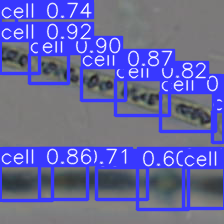
\includegraphics[width=0.5\textwidth]{images/04Implementation/patch.png}
	\caption{Predictions by custom YOLOv5 model on a patch from the test set (image)}
\end{figure}

% \begin{table}
% \centering
% \begin{tabular}{ |l||l|l|l|l|l|l|}
% \hline
% \multicolumn{7}{|c|}{Model Predictions} \\
% \hline
% xmin &        ymin &        xmax &        ymax &  confidence &  class &  name \\
% \hline
% 183.162689 &  167.604874 &  224.000000 &  208.682205 &    0.927962 &      0 &  cell \\
% 0.000000 &   40.554379 &   39.667694 &   73.713120 &    0.924108 &      0 &  cell \\
% 29.663275 &   54.058395 &   68.274818 &   83.056252 &    0.903497 &      0 &  cell \\
% 81.904449 &   67.588310 &  125.853935 &  100.935181 &    0.873414 &      0 &  cell \\
% 0.000000 &  165.740128 &   52.443462 &  200.910339 &    0.864101 &      0 &  cell \\
% 115.671623 &   79.724266 &  169.808105 &  115.588501 &    0.820263 &      0 &  cell \\
% 0.000000 &    0.000000 &   16.820854 &   28.819908 &    0.742437 &      0 &  cell \\
% 39.930126 &  165.439667 &   87.834663 &  199.926498 &    0.709504 &      0 &  cell \\
% 160.140579 &   92.328735 &  215.720291 &  131.021484 &    0.668838 &      0 &  cell \\
% 96.942917 &  167.132019 &  147.778580 &  199.239975 &    0.597954 &      0 &  cell \\
% 137.821564 &  165.580841 &  188.254501 &  209.429321 &    0.481115 &      0 &  cell \\
% 212.847870 &  111.031059 &  223.919052 &  142.591187 &    0.421241 &      0 &  cell \\
% \hline
% \end{tabular}
% \caption{Predictions by custom YOLOv5 model on a patch from the test set
% (DataFrame)}
% \label{dataframe}
% \end{table}

\begin{figure}[h!]
	\centering
	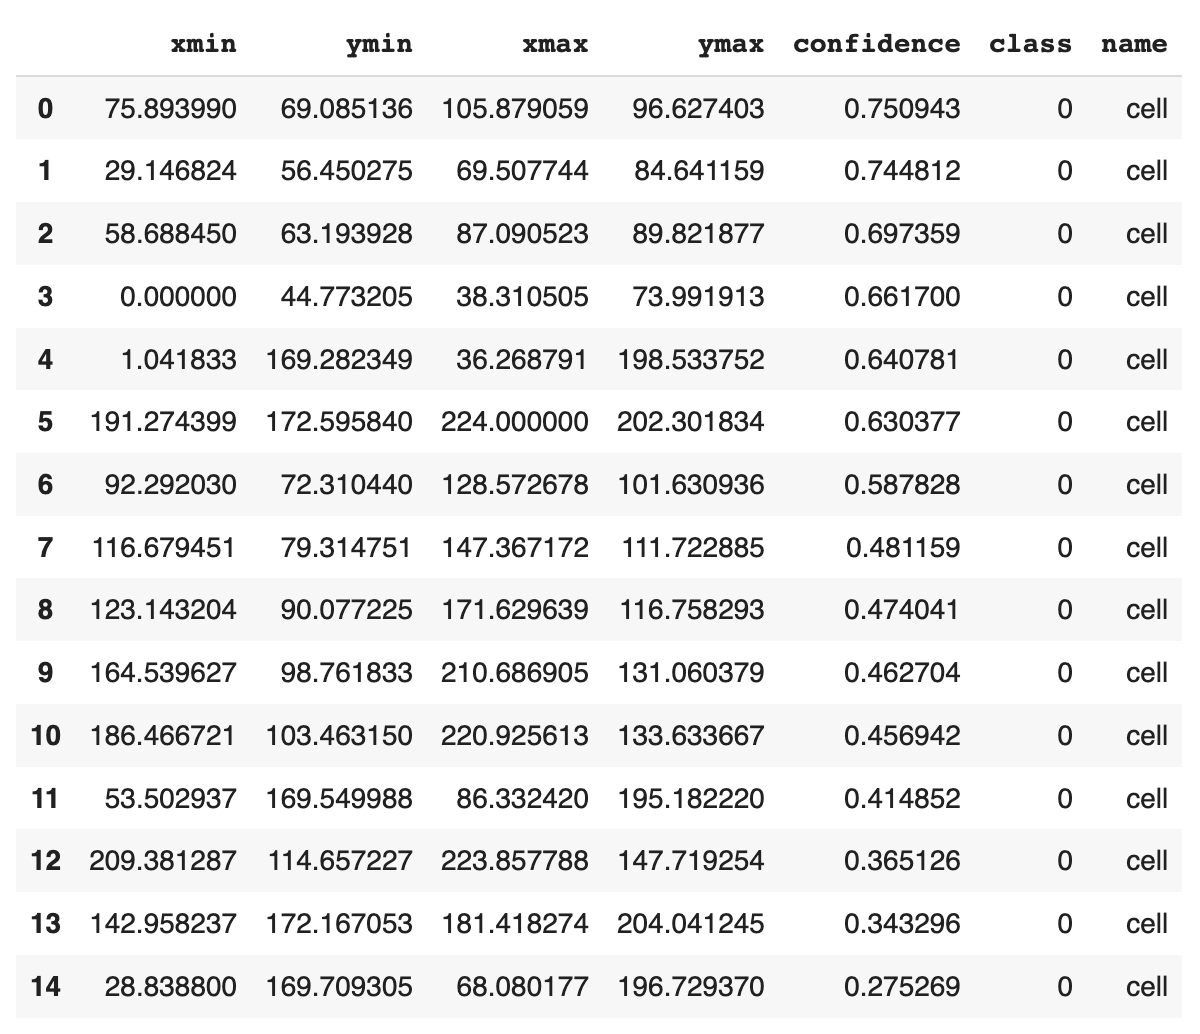
\includegraphics[width=0.8\textwidth]{images/04Implementation/dataframe.png}
	\caption{Predictions by custom YOLOv5 model on a patch from the test set (DataFrame)}
    \label{dataframe}
\end{figure}

\section{Artefact Structure}
A Colab notebook was used to structure the cell counting artefact. This was split into sections and annotated using Markdown to organise all the artefact's components:

\begin{description}
    \item['Preliminaries'] mounts Google Drive, installs and logs into Weights and Biases, and clones YOLOv5 before installing its dependencies.
    
    \item['Training'] simply runs YOLO's \verb|train.py| with the appropriate arguments for \verb|--data|, \verb|--weights|, and other hyperparameters, producing a model.
    
    \item['Counting'] loads a previously trained model and runs \verb`count(...)` using it. This is performed on all 4 images in the test set, returning counts for each.
    
    \item['Evaluation'] computes the model's numerical and percentage error rates for each image, and returns them in a Pandas DataFrame and a LaTeX-format table.
\end{description}

%!TEX root = ../main.tex
%%

\chapter{Testing}
The project's terminal goal of reliable cell counting can be evaluated by the artefact's numerical and percentage count error. Since a detection and localisation network was used, the instrumental goal of the project is to accurately detect and localise cells (in order that they can be counted), and the detection and localisation performance of the underlying model can provide insights into whether the artefact's counts are reached empirically or merely accidentally. The data captured by Weights and Biases during training of a YOLOv5 model includes many metrics for the detection and localisation performance of the model, and provides ample material for qualitative and quantitative evaluation.

\section{Summary}
\subsection{Counting}
Counting accuracy generally improved with each experiment, with the notable exception of Model 2, whose count error was significantly higher than Model 1. Eventually a mean numerical error of 15 and percentage error of around 18\% was achieved by Model 7, the best so far. The counting performance for each model can be seen in Table \ref{count_error}, and Figures \ref{num_error} and \ref{pct_error}.\\

With the exception of Model 1, all models consistently counted more than the ground truth (see Tables \ref{count_1} to \ref{count_7} in the appendix). This was in keeping with the constraint that overcounting is more desirable than undercounting in this use case.\\

\begin{table}
\centering
\begin{tabular}{ |l||l|l|  }
\hline
\multicolumn{5}{|c|}{Count Error} \\
\hline
Model & Num. Error & Pct. Error \\
\hline
1 &      74.25 &   90.767435 \\
2 &      87.00 &  103.001947 \\
3 &      83.25 &  101.850956 \\
4 &      63.00 &   75.363021 \\
5 &      62.50 &   77.071071 \\
6 &      16.00 &   20.892626 \\
\textbf{7} &      \textbf{15.00} &   \textbf{18.237132}\\
\hline
\end{tabular}
\caption{Count error for all models (numerical and percentage)}
\label{count_error}
\end{table}

\begin{figure}[h!]
	\centering
	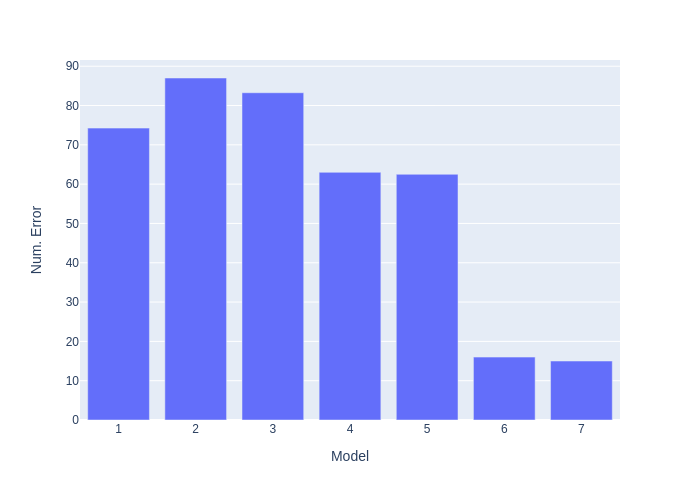
\includegraphics[width=0.8\textwidth]{images/05Testing/num_error.png}
	\caption{Numerical error by model}
	\label{num_error}
\end{figure}

\begin{figure}[h!]
	\centering
	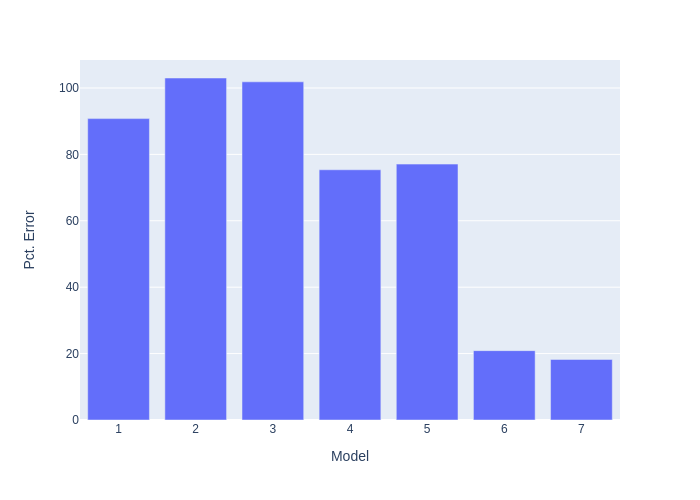
\includegraphics[width=0.8\textwidth]{images/05Testing/pct_error.png}
	\caption{Percentage error by model}
	\label{pct_error}
\end{figure}

\subsection{Metrics}
YOLOv5 produces several metrics to keep track of object detection and localisation performance\footnote{COCO - Common Objects in Context. (no date). Available at: https://cocodataset.org/#detection-eval (Accessed: 05/05/2022).}:\\

\begin{enumerate}
    \item \verb`mAP\_0.5:0.95` (mean average precision for all IoU thresholds from 0.5 to 0.95, step 0.05)
    \item \verb`mAP\_0.5` (mAP at IoU threshold 0.5)
    \item \verb`precision`
    \item \verb`recall`
\end{enumerate}

It was observed during experimentation that YOLOv5's metrics for detection and localisation were of limited relevance in the cell counting task. There was little difference in these metrics between models, despite dramatic changes in count error. In addition, these metrics did not indicate a trend of continuous improvement: some later models' metrics were inferior to those of earlier models which had higher count error. Metrics generally suggested that the models were performing better than their count error and predicted bounding boxes indicated. Notably, mAP metrics improved after Model 1, but this corresponded with a dramatic rise in false positives. It may be the case that increasing mAP simply a result of more false positives.

recall was expected to be far lower for Model 1—which produced a nearly 100\% false negative rate—and precision to be much lower for subsequent models, which produced false positive rates of over 50\%.\\

Initially, the number of epochs was kept low to avoid overfitting, but a key insight gleaned from the model metrics is that training for more epochs does not cause detection and localisation performance to degrade due to overfitting, even after 300 epochs (see Figures \ref{map_0.95}, \ref{map_0.5}, \ref{precision}, and \ref{recall}). In fact, increasing the number of training epochs resulted in dramatic improvements in counting performance.

https://github.com/ultralytics/yolov5/issues/5760

\begin{table}
\centering
\begin{tabular}{ |l||l|l|l|l|  }
\hline
\multicolumn{3}{|c|}{Performance metrics} \\
\hline
Model & mAP\_0.5:0.9 & mAP\_0.5 & precision & recall \\
\hline
1 &      0.44 &   0.77 & 0.77 & 0.68\\
2 &      0.48 &  0.85 & \textbf{0.88} & 0.74 \\
3 &      0.51 &  \textbf{0.91} & \textbf{0.88} & \textbf{0.84} \\
4 &      0.54 & 0.89 & \textbf{0.88} & 0.83 \\
5 &      0.56 & 0.88 & \textbf{0.88} & 0.83 \\
6 &      0.56 & 0.88 & 0.87 & 0.79 \\
7 &      \textbf{0.57} & 0.87 & \textbf{0.88} & 0.82\\
\hline
\end{tabular}
\caption{Performance metrics for all models}
\label{metrics}
\end{table}

\begin{figure}[h!]
	\centering
	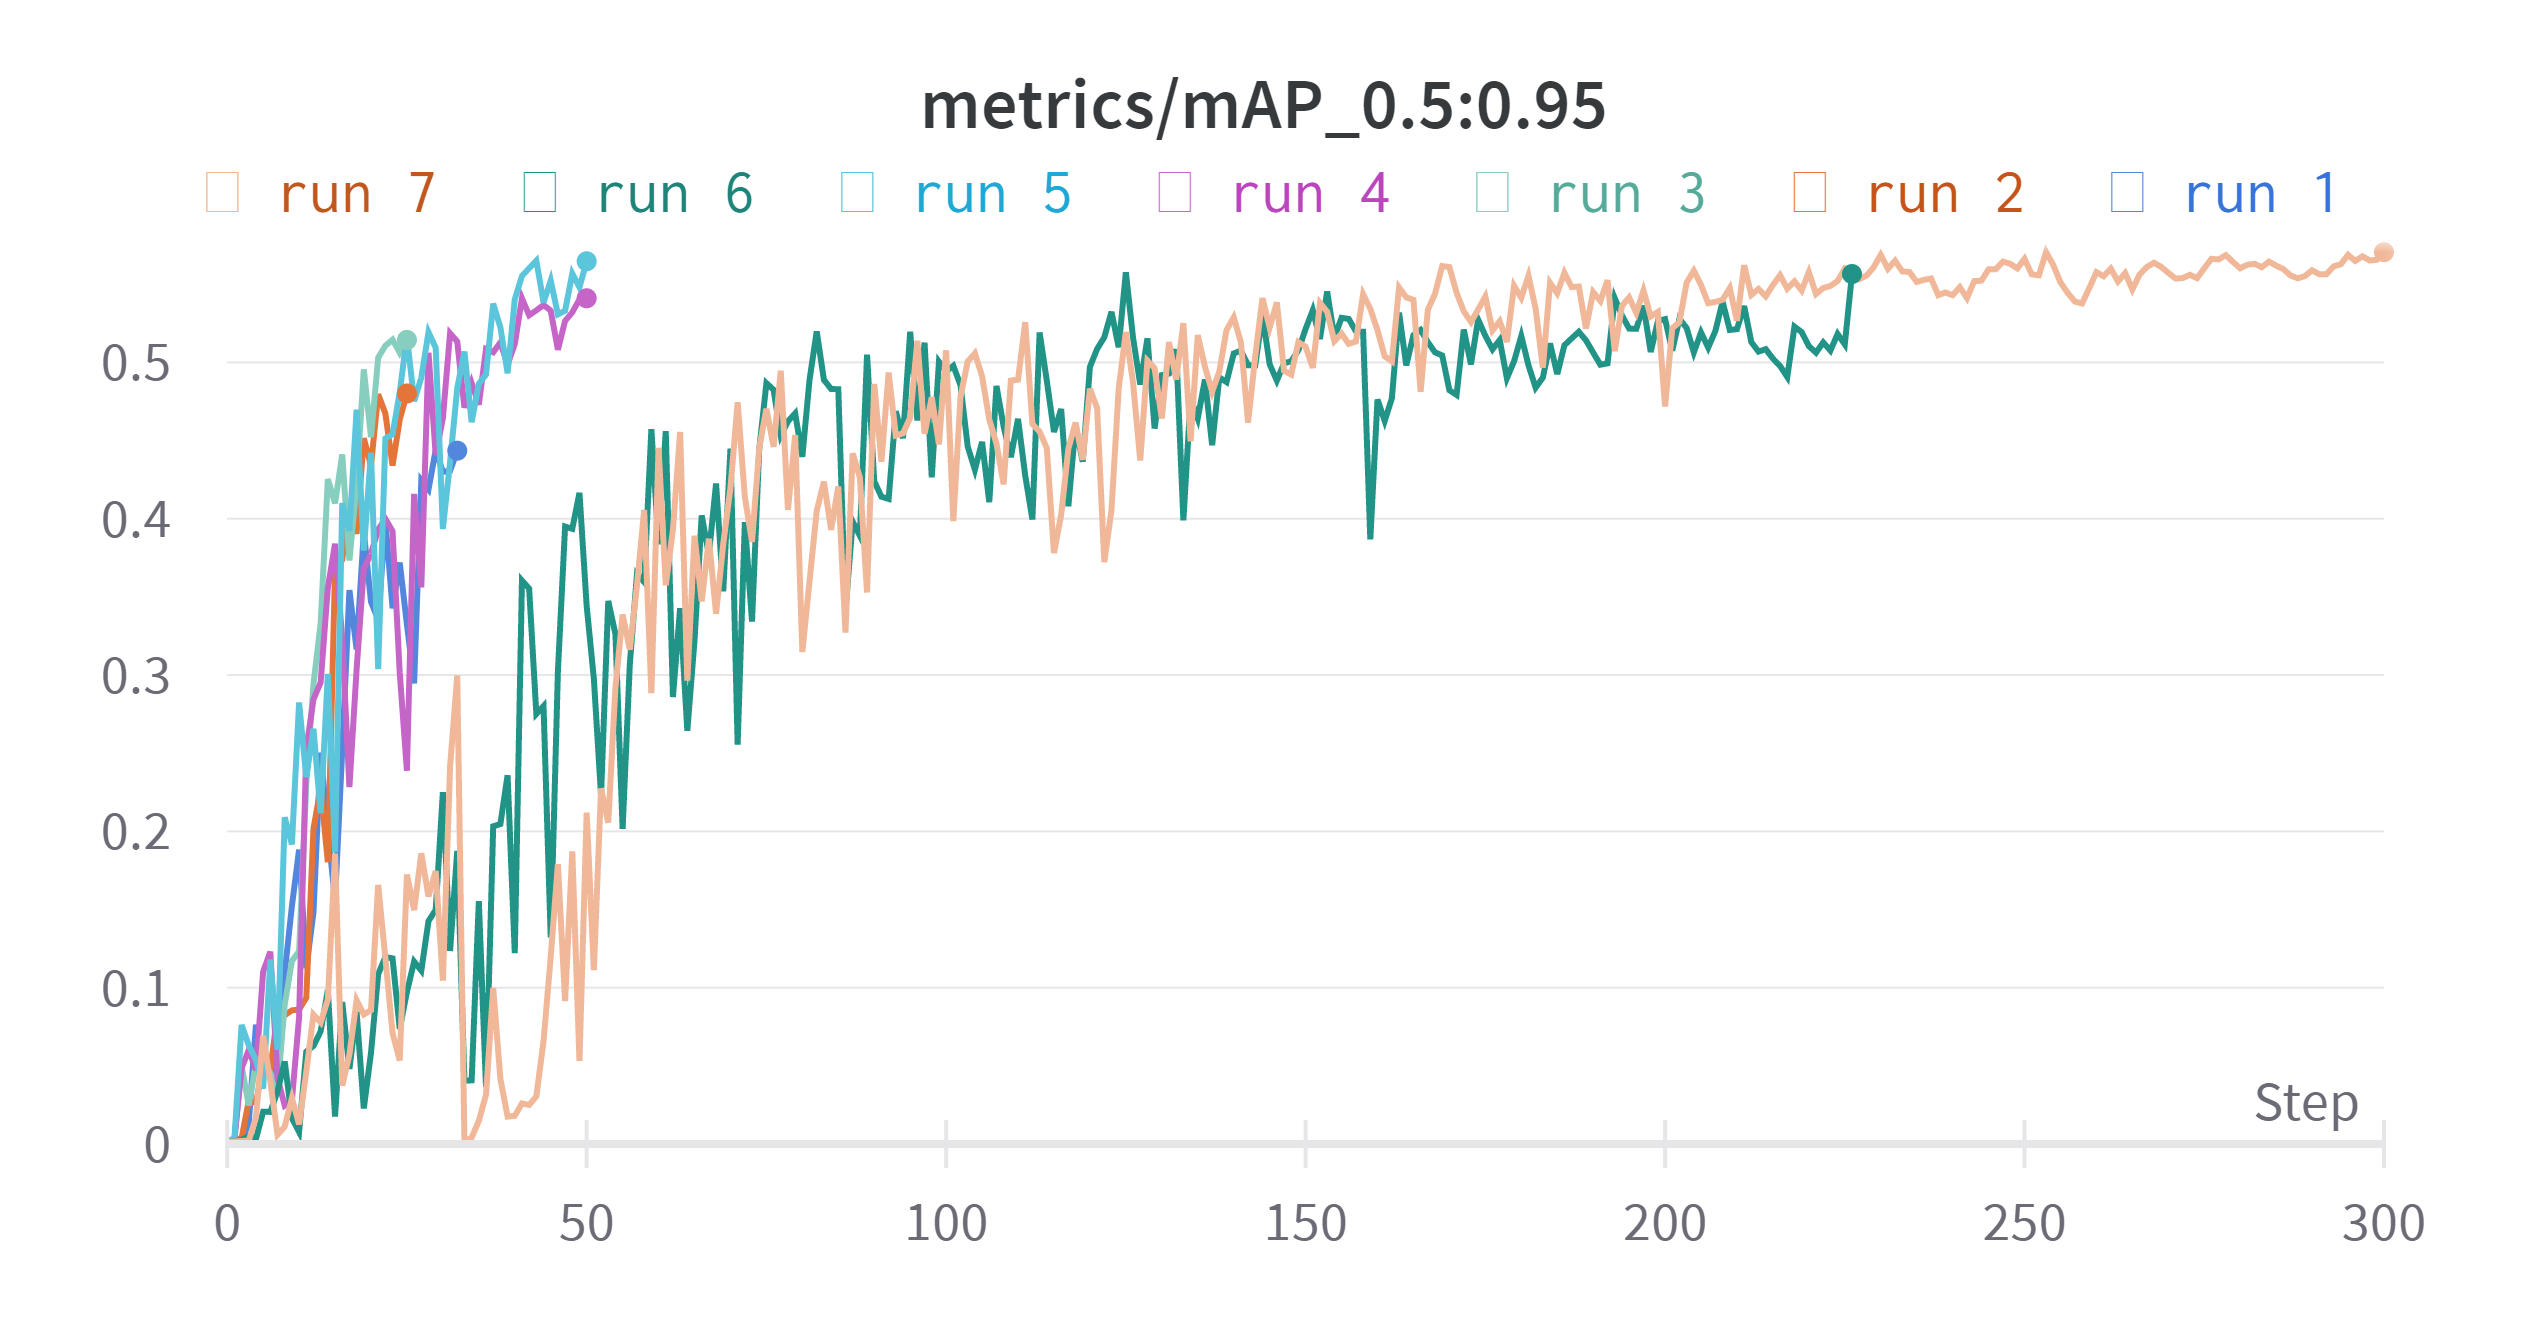
\includegraphics[width=0.8\textwidth]{images/05Testing/map_0.95.png}
	\caption{mAP\_0.5:0.95}
	\label{map_0.95}
\end{figure}

\begin{figure}[h!]
	\centering
	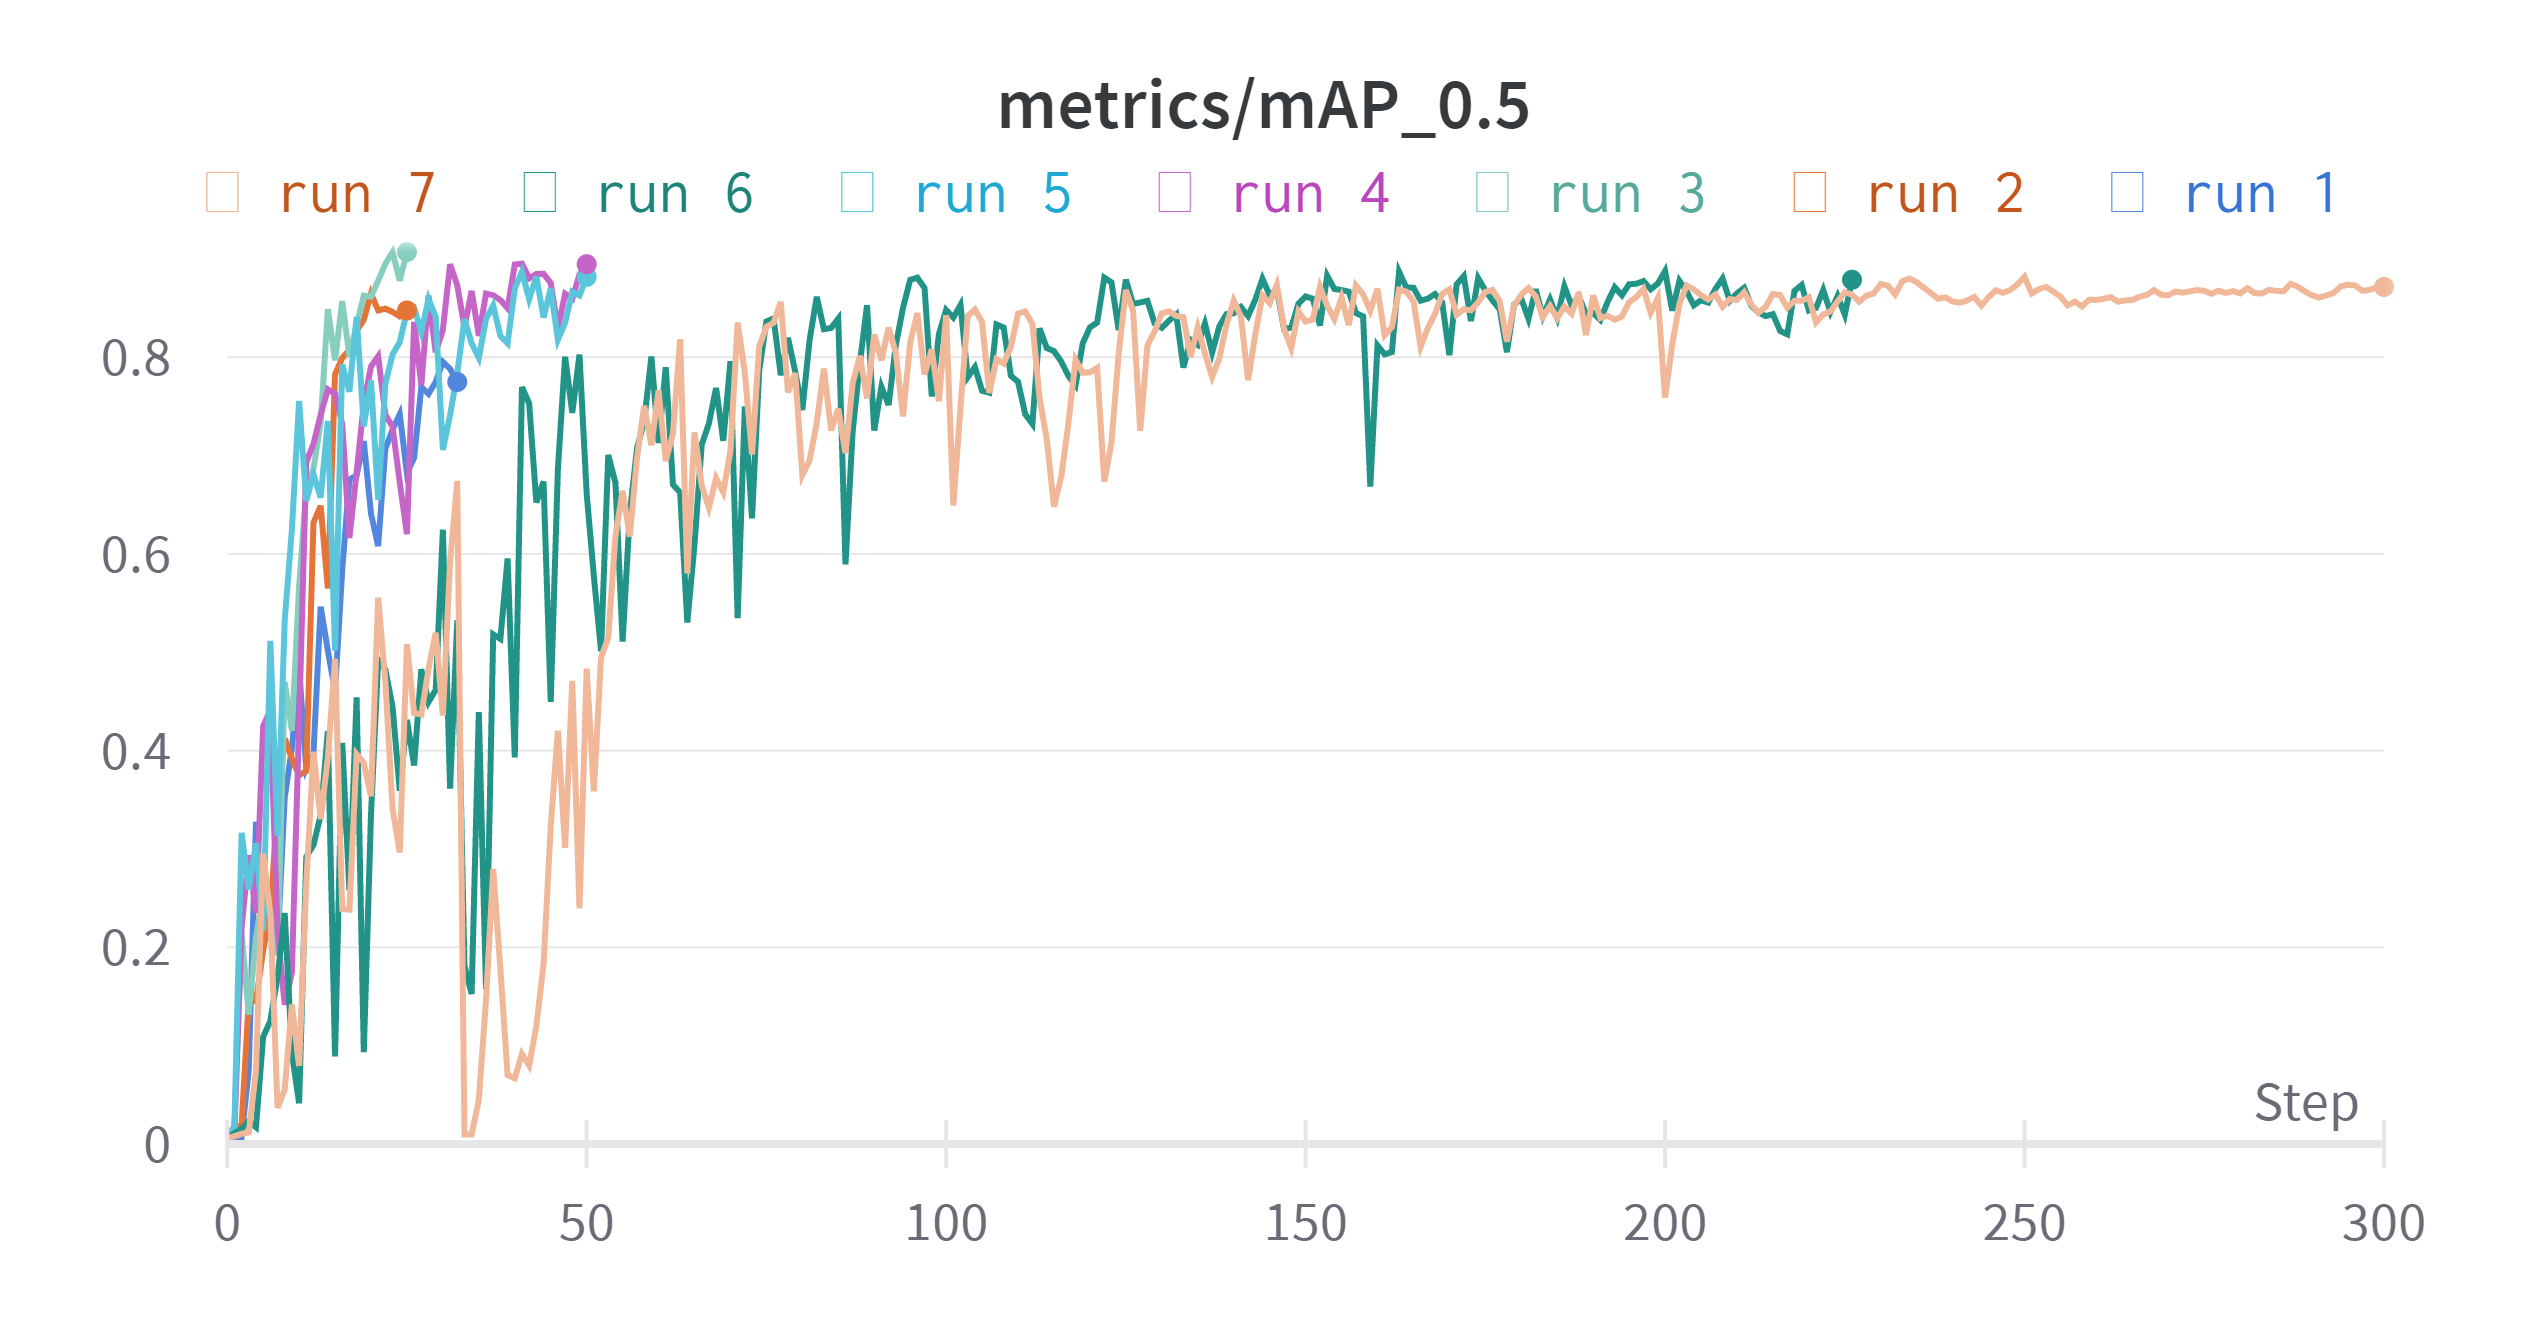
\includegraphics[width=0.8\textwidth]{images/05Testing/map_0.5.png}
	\caption{mAP\_0.5}
	\label{map_0.5}
\end{figure}

\begin{figure}[h!]
	\centering
	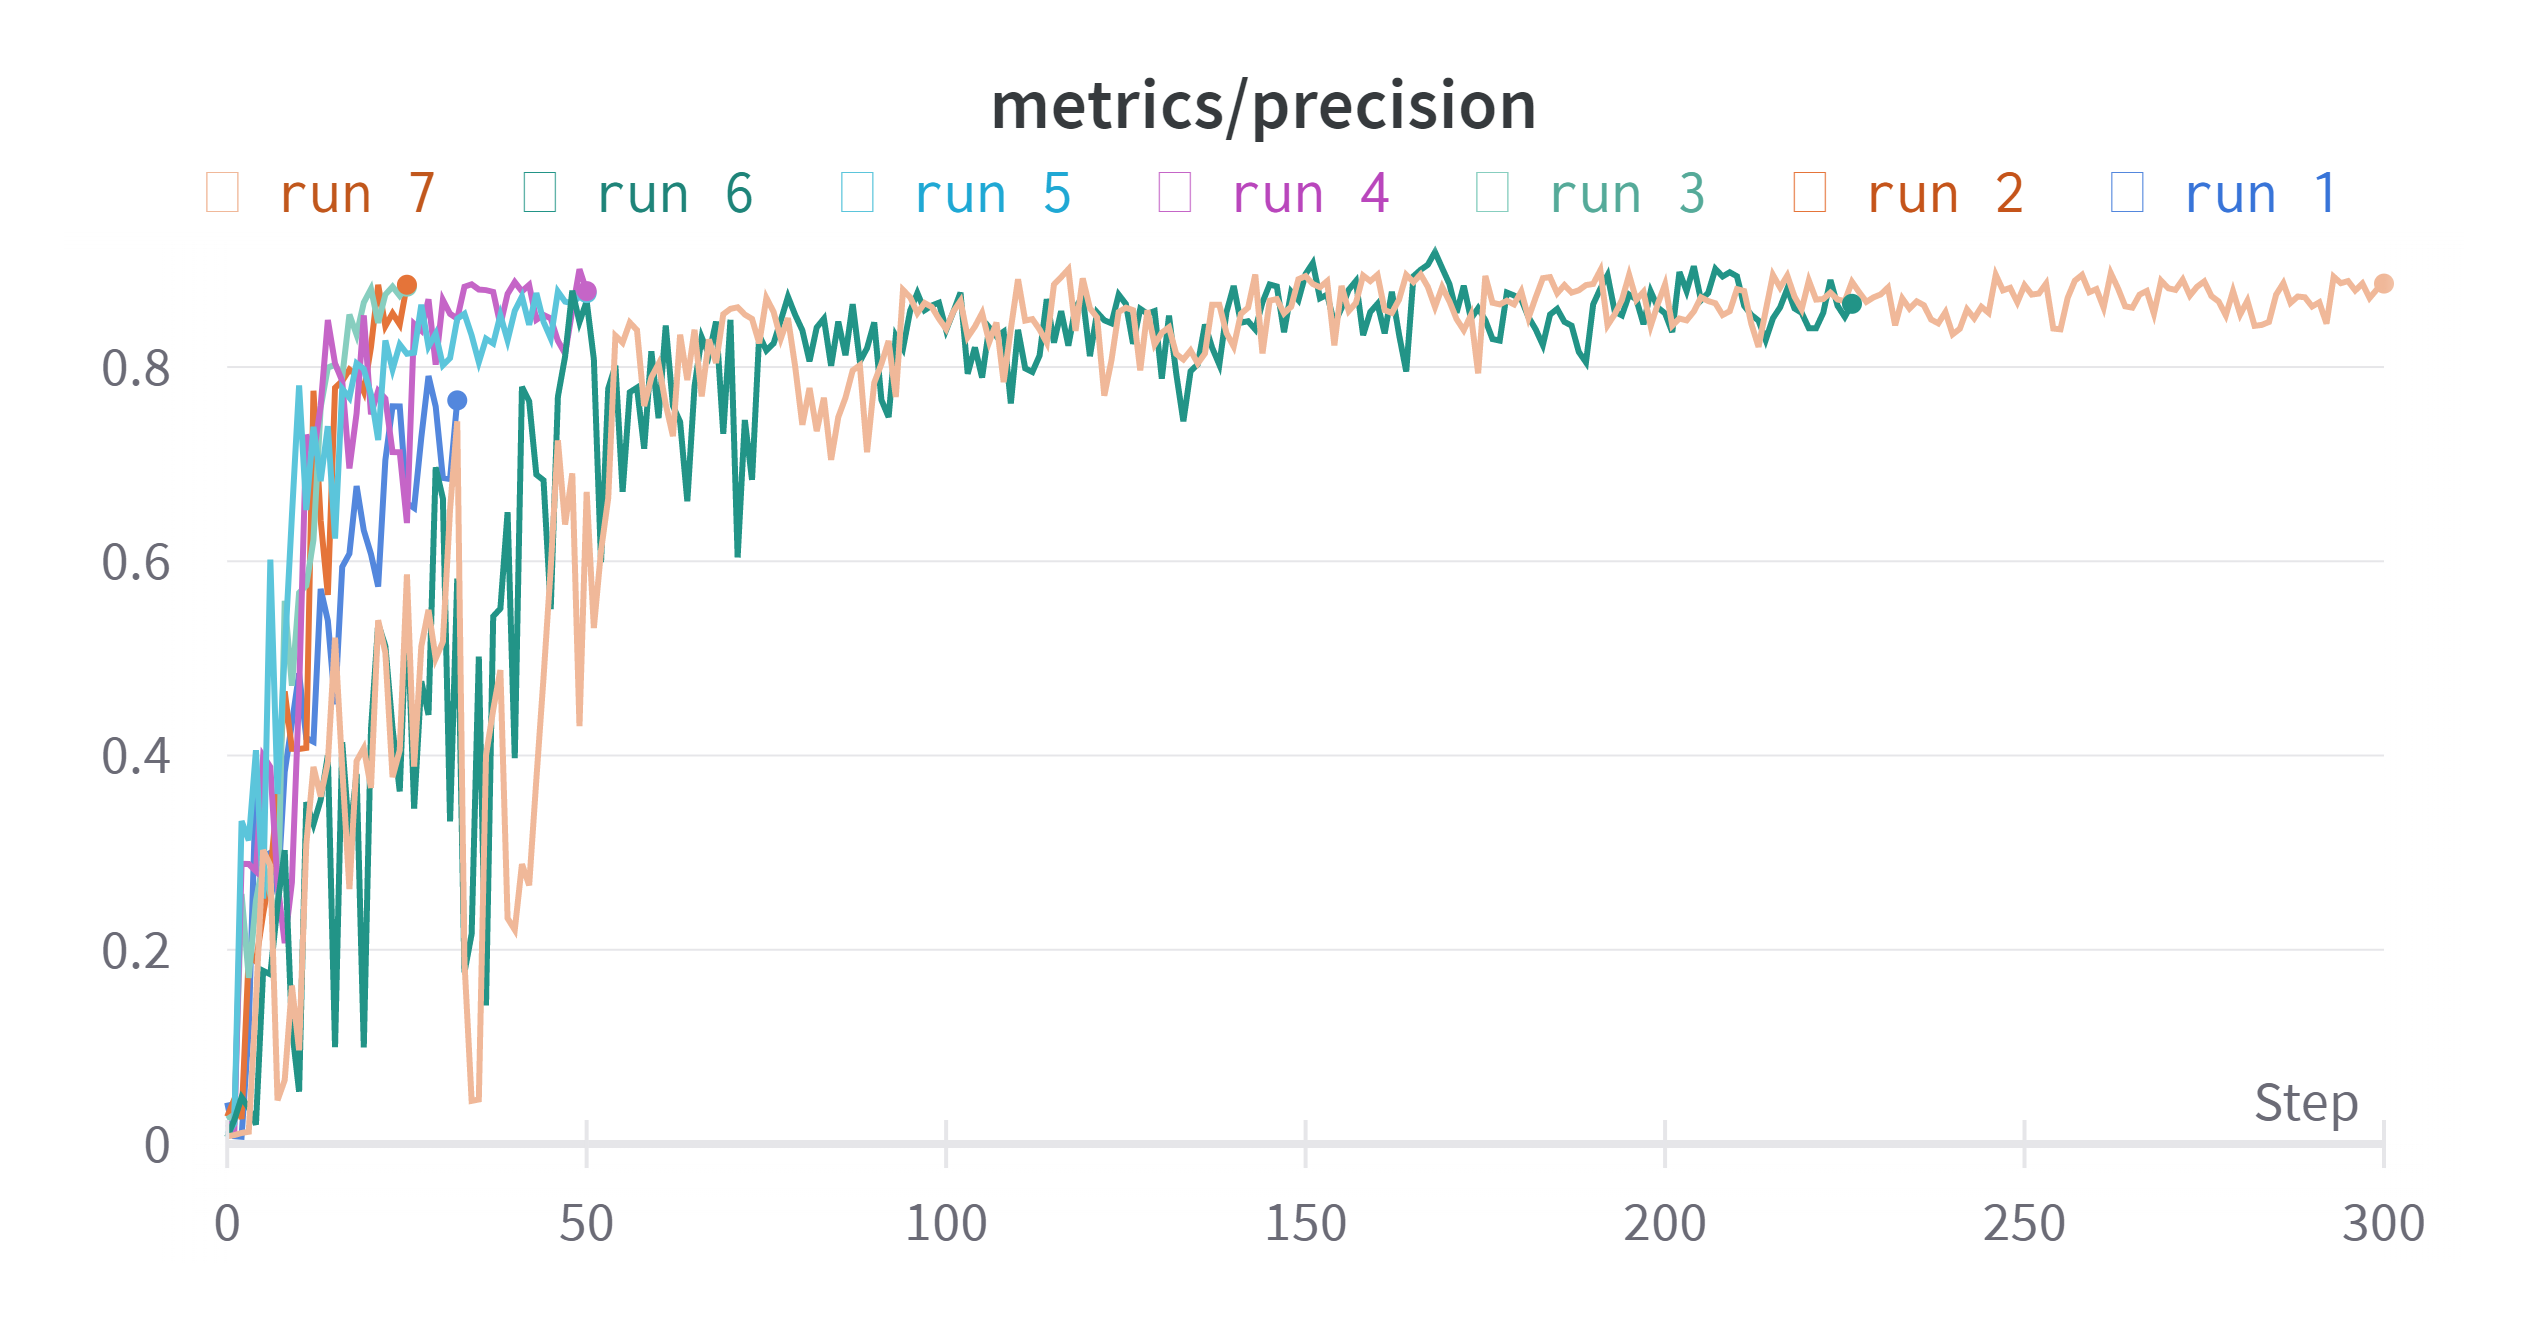
\includegraphics[width=0.8\textwidth]{images/05Testing/precision.png}
	\caption{precision}
	\label{precision}
\end{figure}

\begin{figure}[h!]
	\centering
	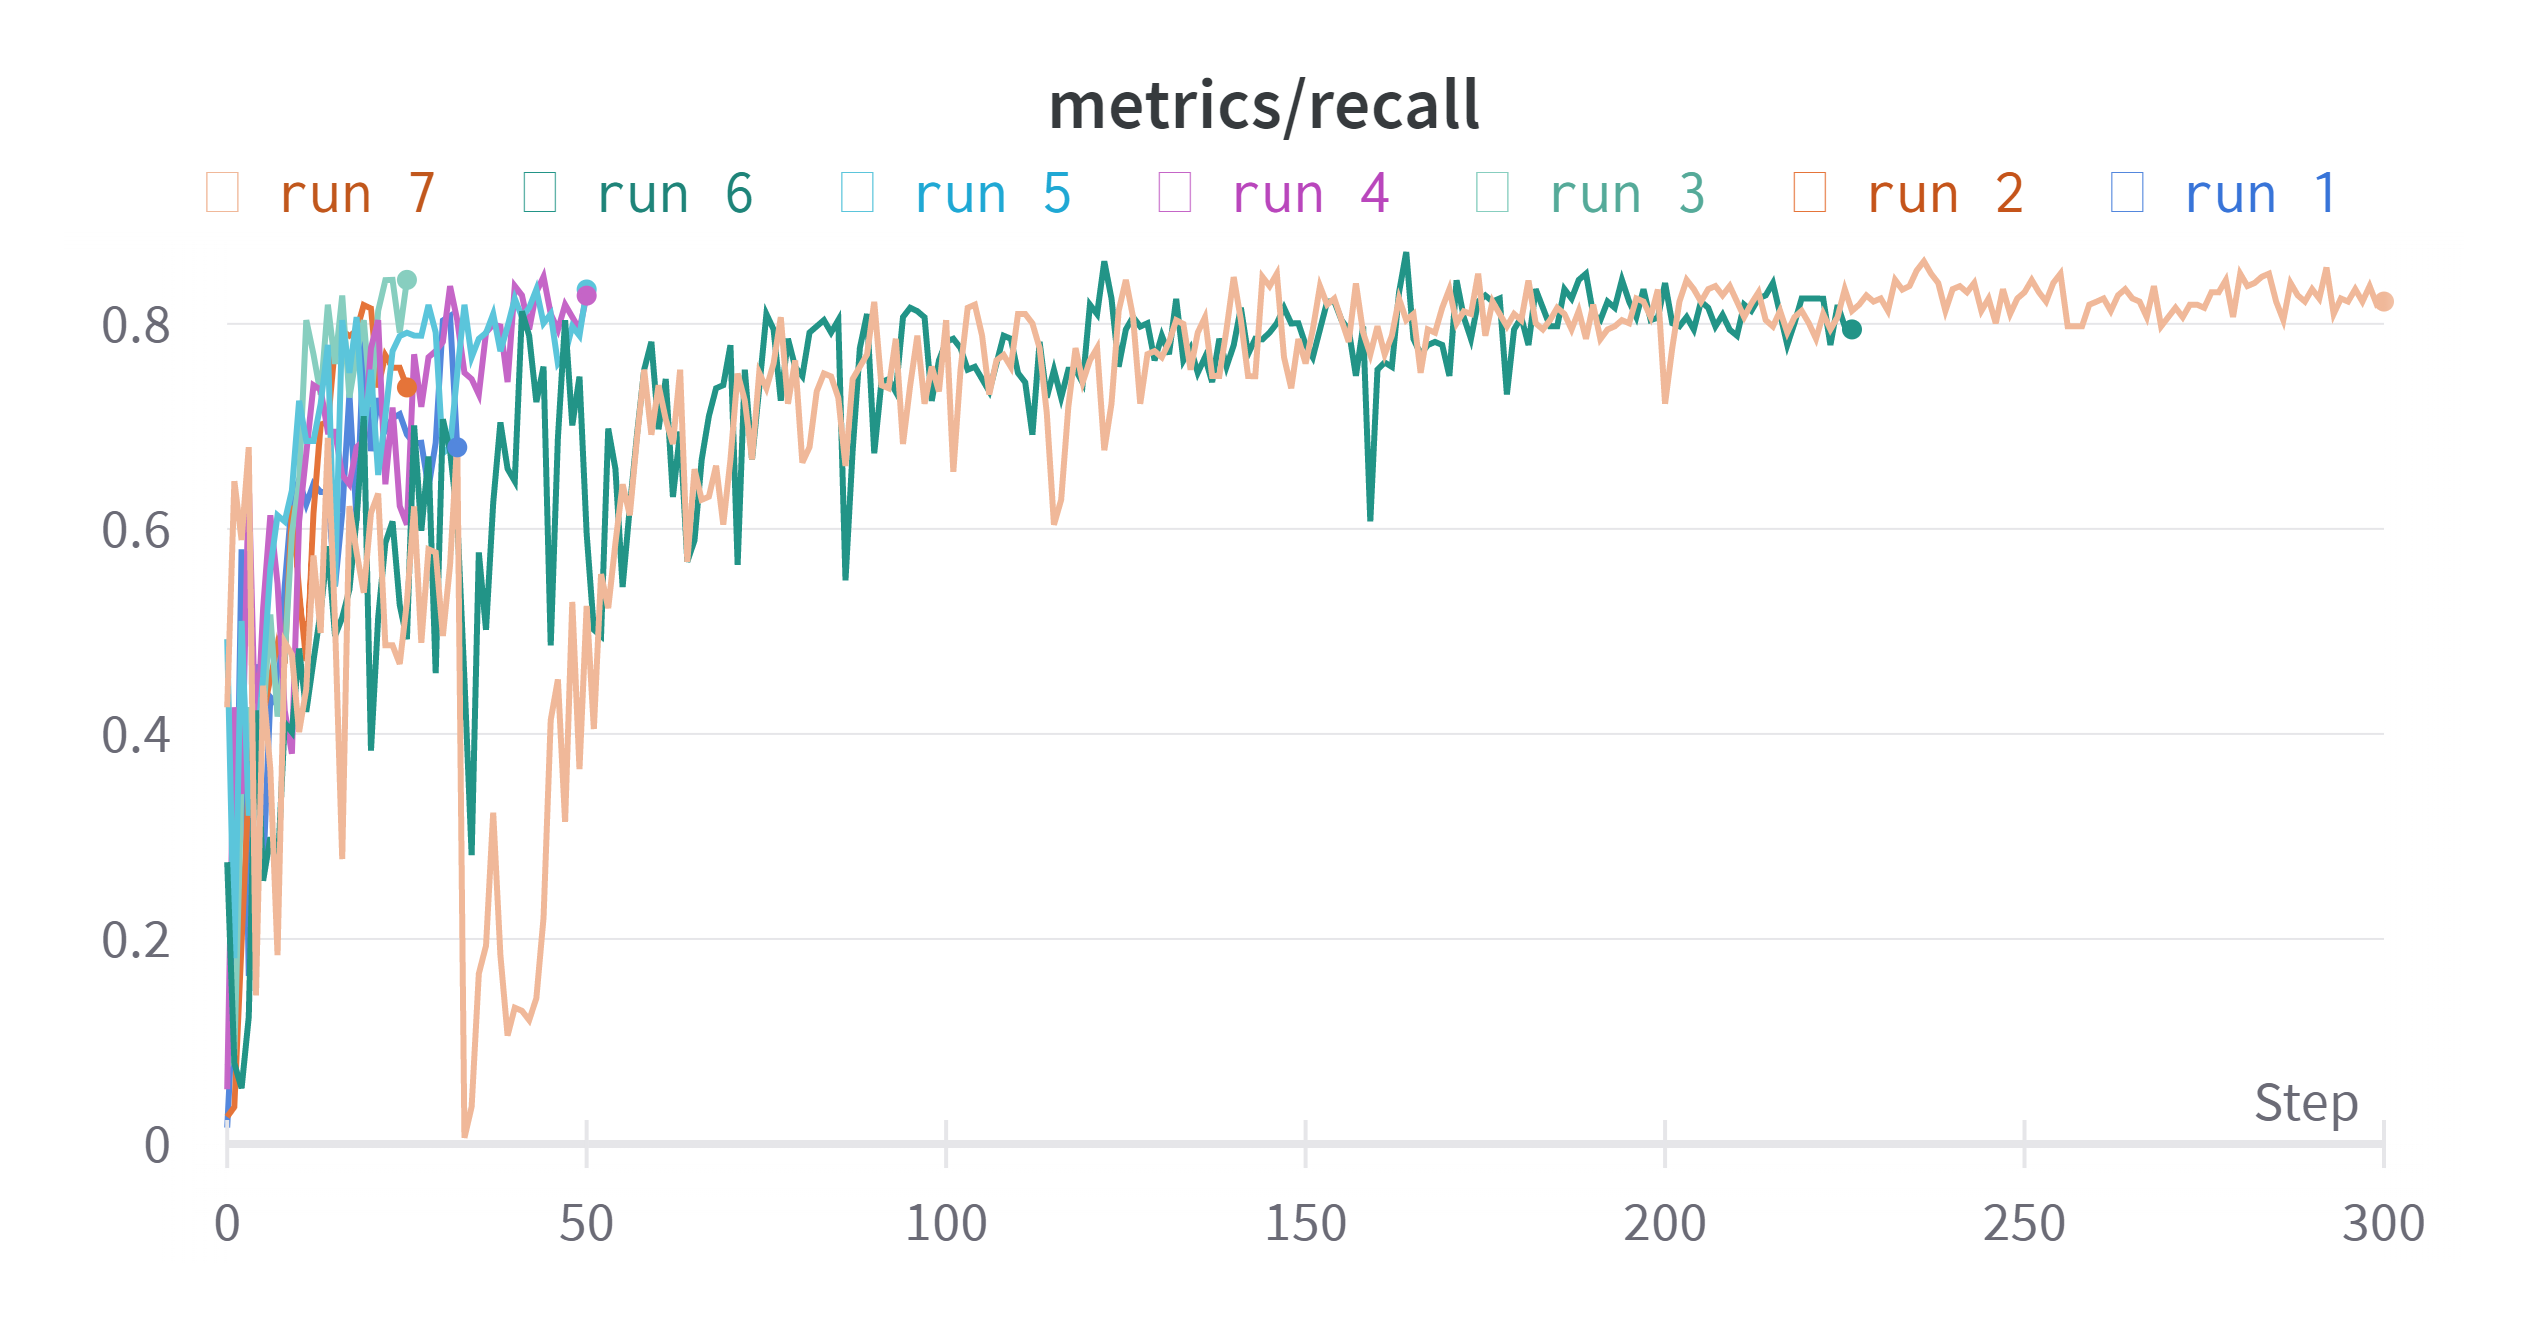
\includegraphics[width=0.8\textwidth]{images/05Testing/recall.png}
	\caption{recall}
	\label{recall}
\end{figure}

\section{Model 1}
Experiment 1 commenced testing with disappointing results. The model consistently undercounted, detecting very few cells and demonstrating a count error of nearly 100\% (see Figure \ref{count_error}). This can be attributed to the model's poor localisation capabilities as seen in Figure \ref{model1}: few cells are detected, and those which are are predicted with low confidence. This suggested that the configuration for Experiment 1 was flawed, and did not allow the model to learn enough about the target class to make accurate predictions.\\

\begin{figure}
\subfloat{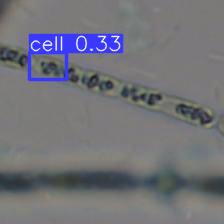
\includegraphics[width=3in]{images/05Testing/run01/easy}}
\subfloat{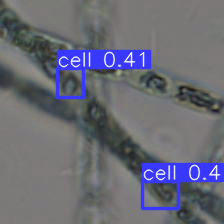
\includegraphics[width=3in]{images/05Testing/run01/hard}}
\caption{Predictions on 'easy' (left) and 'hard' (right) images from the test set by Model 1}
\label{model1}
\end{figure}

\section{Model 2}
The poor performance of Model 1 prompted a revision of the dataset annotations, which were revised from the sparse Version 1 to Version 2. Version 2 included far more cells, including those which were less clearly depicted. It was hypothesised that this change would provide the model with sufficient information to generalise across different levels of image clarity.\\

From Model 2 onwards, the undercounting problem was reversed: all models following Model 1 consistently \textit{over}counted, initially with errors of more than 100\%. This reversal cannot be attributed to one change alone between Experiments 1 and 2—both the batch size (16 to 32) and the number of epochs (32 to 25) were changed—but these changes were insignificant compared to the overhaul of the dataset annotations. It seemed that the resulting model was highly vulnerable to producing false positives and counting the same cells twice, and this was confirmed by qualitative evaluation of the model's predicted bounding boxes (see Figure \ref{model2}). This suggested that the revision of the dataset annotations was the most likely cause of the dramatic difference in count error between Models 1 and 2.\\

While the error for Model 2 was greater than that of Model 1, making Model 2 strictly the 'worse' model, it was also taken into account that the implications of deploying an undercounting model such as Model 1 would be more serious than one which overcounted, such as Model 2. While the revision of the dataset annotations was seen as the likely reason for Model 2's overcounting, it was decided to err on the side of more annotation, since overcounting is more desirable than undercounting.

\begin{figure}
\subfloat{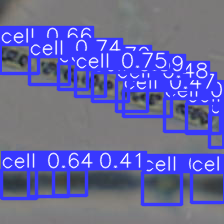
\includegraphics[width=3in]{images/05Testing/run02/easy}}
\subfloat{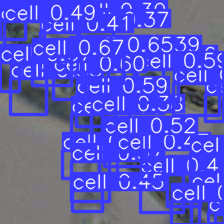
\includegraphics[width=3in]{images/05Testing/run02/hard}}
\caption{Predictions on 'easy' (left) and 'hard' (right) images from the test set by Model 2}
\label{model2}
\end{figure}

\section{Model 3}
For the third experiment, the proportion of the dataset used for training was increased by 20\% for a train/test/val split of 70/15/15. It was theorised that Model 2's overcounting problem might be ameliorated by providing the model with more data to learn from. In addition, the dataset annotations were revised to Version 3, which added cells which were both out-of-focus and not fully within the patch, and occluded cells.\\

This model showed marginal improvement in count error compared to Model 2. Since both of the changes to the configuration were made simultaneously, it is unclear whether either change, in isolation, might have yielded substantial improvement or deterioration. In particular, the significance of enlarging the training set could be investigated in isolation, since the previous revision to the dataset annotations yielded reduced accuracy. This might have counteracted any positive effect of the larger training set in this case.

\section{Model 4}
The only change made to the configuration for Experiment 4 was to increase the number of epochs (30 to 50). This resulted in a sharp reduction in count error, greater than that seen in Experiment 3. 

\begin{figure}
\subfloat{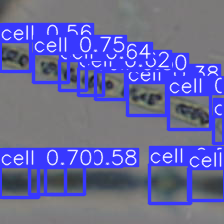
\includegraphics[width=3in]{images/05Testing/run04/easy}}
\subfloat{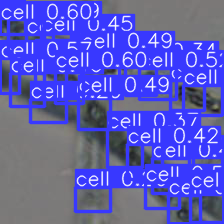
\includegraphics[width=3in]{images/05Testing/run04/hard}}
\caption{Predictions on 'easy' (left) and 'hard' (right) images from the test set by Model 4}
\label{model4}
\end{figure}

\section{Model 5}
Model 5 was fine-tuned on a significantly more complex base model than previous models (YOLOv5l). This change had a negligible benefit for numerical count error, and in fact increased count percentage count error.

\section{Model 6}
Experiment 6 dramatically increased the number of epochs (50 to 300) and batch size (32 to 128), after the success of Experiment 4 and on the recommendation of the YOLOv5 documentation\footnote{Tips for Best Training Results · ultralytics/yolov5 Wiki. (no date). Available at: https://github.com/ultralytics/yolov5/wiki/Tips-for-Best-Training-Results (Accessed: 05/05/2022).}. The base model was also changed back to YOLOv5s. These changes had the most dramatic effect on the model's count error of all those made during experimentation, resulting in substantial improvement.

\begin{figure}
\subfloat{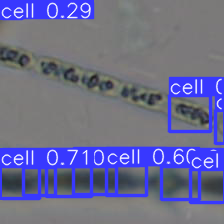
\includegraphics[width=3in]{images/05Testing/run06/easy}}
\subfloat{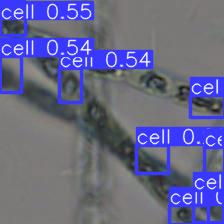
\includegraphics[width=3in]{images/05Testing/run06/hard}}
\caption{Predictions on 'easy' (left) and 'hard' (right) images from the test set by Model 6}
\label{model6}
\end{figure}

\section{Model 7}
Experiment 7 again changed the base model from YOLOv5s to YOLOv5l. Using this more complex model resulted in only marginally greater counting accuracy than the YOLOv5s-based Model 6.

\begin{figure}
\subfloat{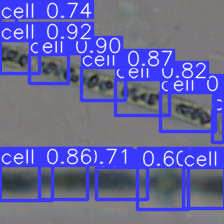
\includegraphics[width=3in]{images/05Testing/run07/easy}}
\subfloat{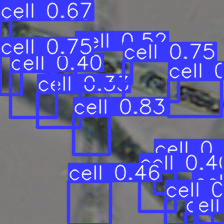
\includegraphics[width=3in]{images/05Testing/run07/hard}}
\caption{Predictions on 'easy' (left) and 'hard' (right) images from the test set by Model 7}
\label{model7}
\end{figure}

%!TEX root = ../main.tex
%%

\chapter{Evaluation}
\section{Requirements Evaluation}
The project requirements specified 20 requirements,with 14 of these having a priority of 'Must' or 'Should'. Of the 8 'Must' requirements, 7 were unambiguously achieved. One 'Must' requirement contained an ambiguity: 'As an output, produce a reliable count of cells in the image'. This requirement could be said to be more or less fulfilled: the artefact certainly returns a count, but whether this count is 'reliable' is itself subject to further evaluation.\\

Of the 6 'Should' requirements, 3 were unambiguously fulfilled. The project used a deep CNN model to perform detection-based counting of cells, and was backed up to a GitHub repository. 'Process an input image quickly at test time' was also considered to be unambiguously fulfilled, since it specified a maximum acceptable processing time of 1 minute (inference with Model 7 takes around 1 second). Other requirements were arguably more or less fulfilled: it is unlikely that the artefact 'Use(d) the optimal hyperparameters for the model', but this is unfalsifiable without future experimentation. 'Process training data quickly at train time' is ambiguous: the training of Model 7 took 21 minutes and 48 seconds, but no benchmark figure for 'quickly' is provided to compare this against. Only 1 'should' requirement was unambiguously not achieved: the artefact was not fully functional by the due date of the Proof of Concept deliverable.\\

6 'Could' requirements were also specified, but 4 of these simply listed conflicting options for project methodology, of which 1 was ultimately chosen ('Use the Pytorch implementation of YOLOv5). Of the 2 remaining, one was fulfilled: in addition to a count, the artefact 'Produce(s) a secondary output for explanation purposes'. This takes the form described in the requirement: an image patch from the input, with predicted bounding boxes.\\

These can be compared with the state of the art as described in \cite{xie2018microscopy} and \cite{Identification-and-enumeration-of-cyanobacteria}.


\section{Methodology}
One of the key limitations of the project was that several changes at a time were often made to the training configurations.\\

The number of epochs was kept low in early experiments to prevent overfitting, but this countermeasure proved to be unnecessary. Later models trained for 300 epochs without overfitting, and in fact increasing the number of epochs resulted in significant reductions in count error, more than any other change to experiment configurations. A minimum of 300 epochs is suggested by the YOLOv5 documentation\footnote{Tips for Best Training Results · ultralytics/yolov5 Wiki. (no date). Available at: https://github.com/ultralytics/yolov5/wiki/Tips-for-Best-Training-Results (Accessed: 05/05/2022).}, so this should have been a natural starting point, but this resource was not discovered until late in the project.

The YOLOv5 wiki also recommends more than 1500 images per class, with a minimum of 10,000 instances per class also recommended. Since 640 patches have already been annotated over the course of 3 hours, annotation of another 860 patches would take a single annotator approximately 4 hours.

Using image patches itself presented problems, most notably the fact that cells which straddled the edge of a patch were counted twice before the counting component was modified to control for this. An alternative method of evaluating the model's counting performance without this potentially biasing addition might be to calculate count error per-patch and average this over the image, but since ground truth counts are provided only for the full images, these would need to be calculated for each patch.

The dataset is potentially problematic. Only one labeller was 

\section{Results}


Label consistency - affects precision and recall

More background images to reduce false positives

Future experiments would likely start with 300 epochs, as specified in the YOLOv5 documentation.

Different model?
Dataset not perfect-1 labeller
Patches caused problems with counting twice

The most likely way to improve the model's results is


%!TEX root = ../main.tex
% %

\chapter{Conclusion}
This project investigated the application of neural network models, specifically those for object detection and localisation, to the counting of filamentous cyanobacteria cells. Counting these cells in this way is novel. A methodology was devised to run iterative experiments, training 7 neural network models with varying combinations of configurations and parameters, which led to progressively improving results. The best model ultimately allowed the cell counting artefact to achieve an average of 20\% percentage error on the test set. REQUIREMENTS\\

The project demonstrates that neural network models for detection and localisation can be successfully applied to the task of cell counting, with few training data.

\section{Future Work}
The project methodology⁠ could be improved in a number of ways. Firstly, any future experimentation should isolate all changes to the training configuration, training a new model for each change. This will allow the change responsible for any improvement or decline in performance to be clearly identified.\\

The subset used of the full Micropics dataset is relatively small, so a much richer dataset could be created by annotating the remaining images in Micropics. Even an increase in the number of 'empty' images containing only slide backgrounds would improve the model\footnote{Tips for Best Training Results · ultralytics/yolov5 Wiki. (no date). Available at: https://github.com/ultralytics/yolov5/wiki/Tips-for-Best-Training-Results (Accessed: 05/05/2022).}, and more of these would be trivial to produce. Further annotation should ideally be undertaken by multiple annotators, and by specialists in the identification and differentiation of filamentous cyanobacteria cells. Annotation supported by domain expertise would significantly improve the validity of the project.\\

Since detection and localisation models are always improving, attempts could be made to make the artefact more network-agnostic, since it currently counts only with YOLOv5. If a future network exceeds the detection and localisation performance of YOLOv5 with similar or better training and inference speeds, it should be possible to swap YOLOv5 for this superior model.\\



Since cells in the dataset are highly variable⁠—varying in shape, size, and orientation, and appearing in different levels of image clarity⁠—this presents an opportunity to use data augmentation to improve the artefact's ability to generalise. This may be particularly useful given that the dataset is small.

More epochs
Greater batch size
More complex model 


\nocite{*} %Take this out if you don't want it to show all the references but only the ones you've referenced 
\bibliography{references}




%!TEX root = ../main.tex
% %

\begin{appendices}

\section{Results by Model}
\subsection{Model 1}

\begin{table}[h!]
\centering
\begin{tabular}{||c c c c c||} 
\hline
Image &  Ground Truth &  Model Count &  Num. Error &    \% Error \\
\hline\hline
37 &            81 &            7 &          74 &  91.358025 \\
39 &            58 &            6 &          52 &  89.655172 \\
41 &            86 &            7 &          79 &  91.860465 \\
44 &           102 &           10 &          92 &  90.196078 \\
\hline
\end{tabular}
\caption{Counts \& errors for Model 1}
\label{count_1}
\end{table}

\begin{figure}[h!]
\subfloat{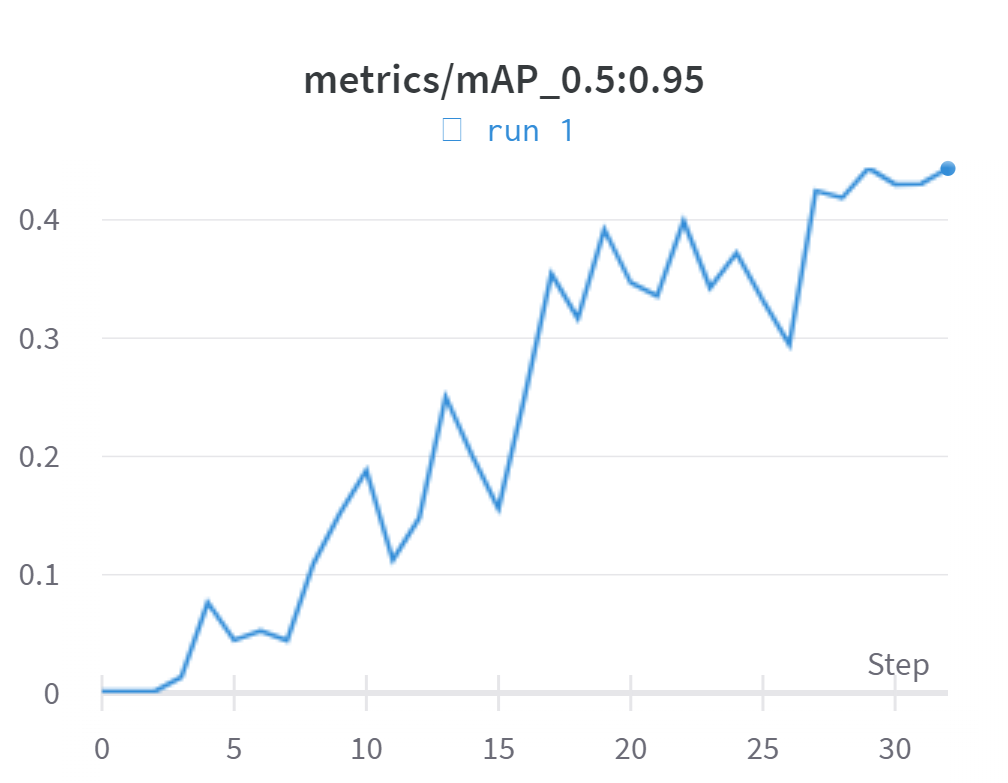
\includegraphics[width=3in]{images/05Testing/run01/Section-2-Panel-0-l24a15v4n}}
\subfloat{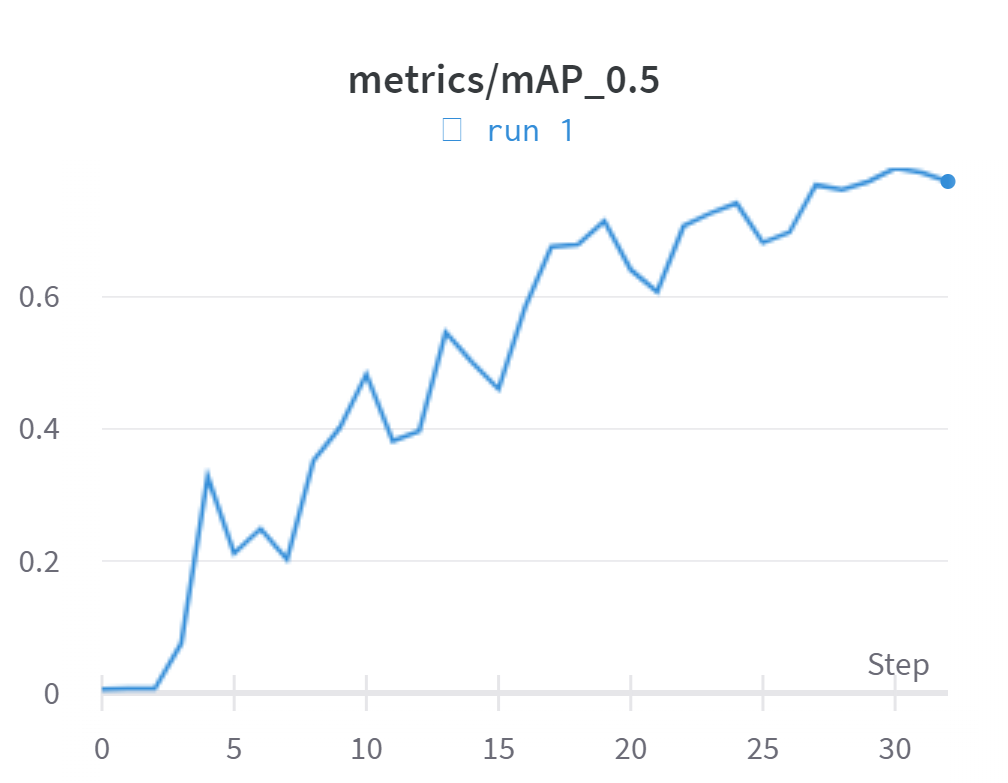
\includegraphics[width=3in]{images/05Testing/run01/Section-2-Panel-1-xq6pmkk16}}\\
\subfloat{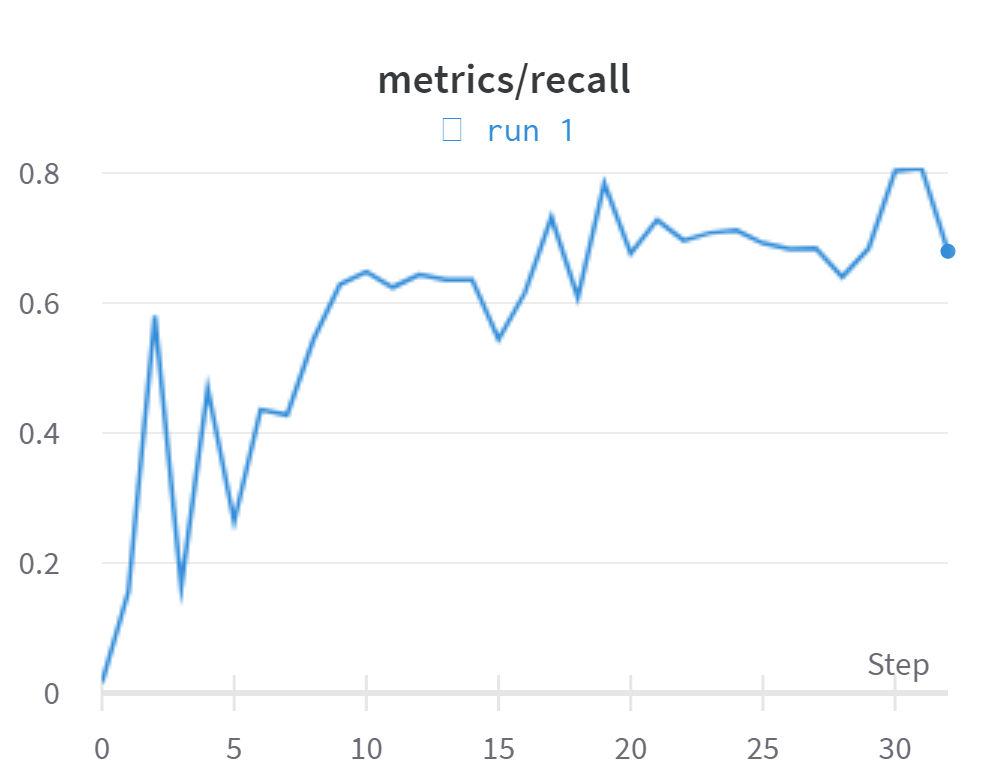
\includegraphics[width=3in]{images/05Testing/run01/Section-2-Panel-2-45rd7tgay}}
\subfloat{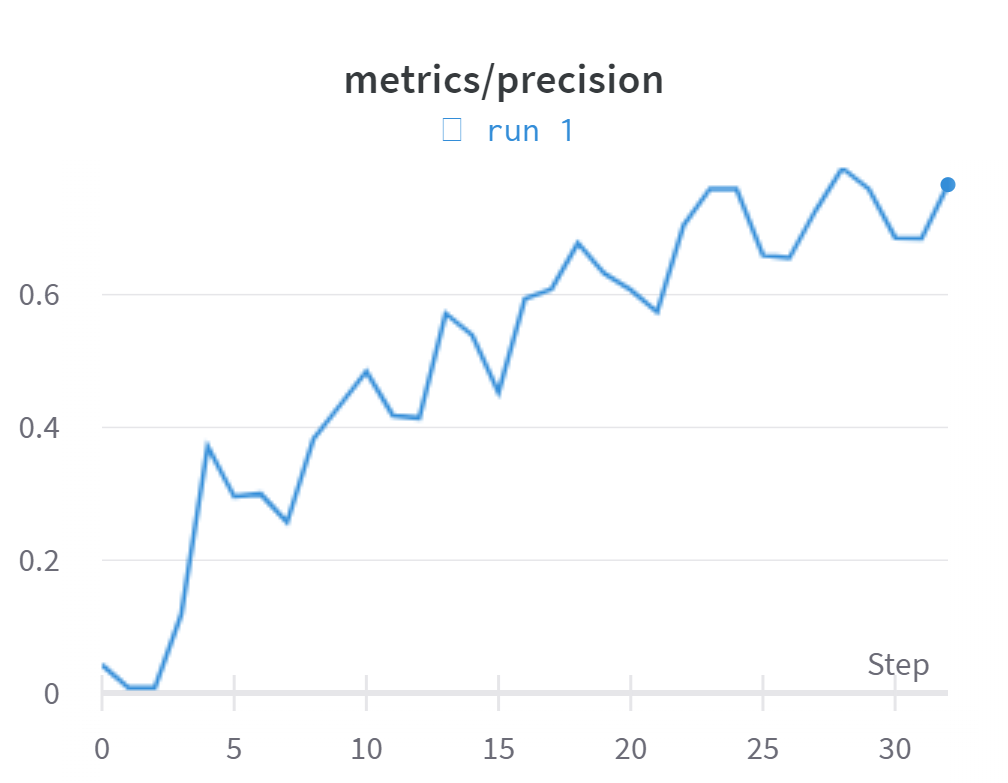
\includegraphics[width=3in]{images/05Testing/run01/Section-2-Panel-3-jsgjesr4f}}\\
\subfloat{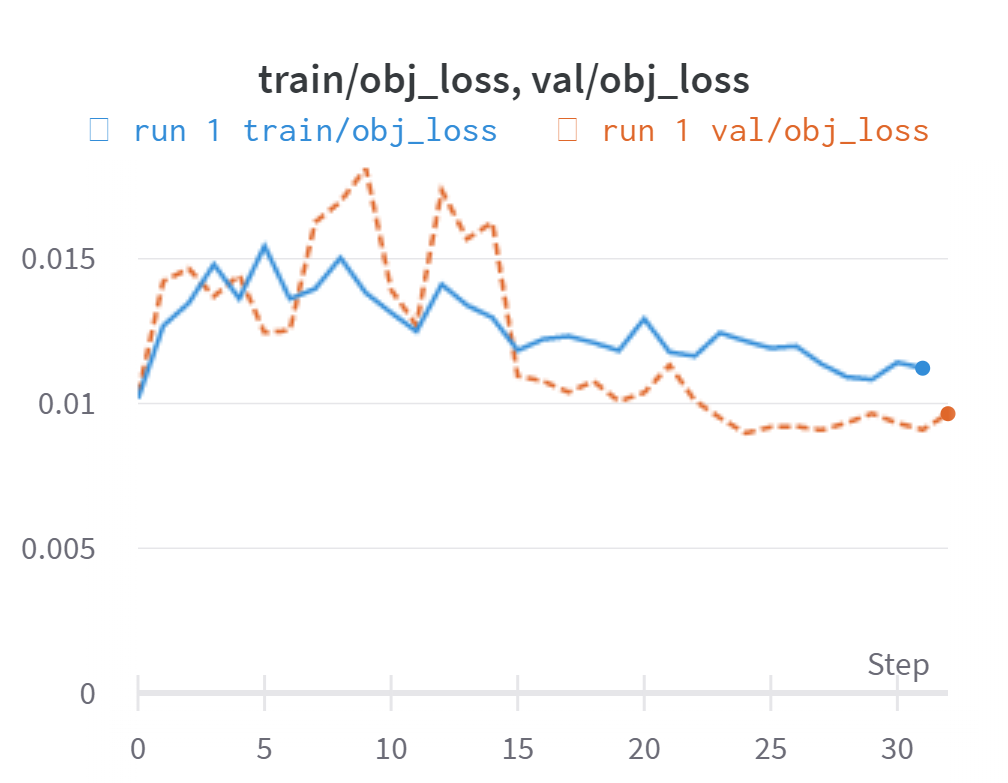
\includegraphics[width=3in]{images/05Testing/run01/Section-2-Panel-4-jgehu72sd}}
\subfloat{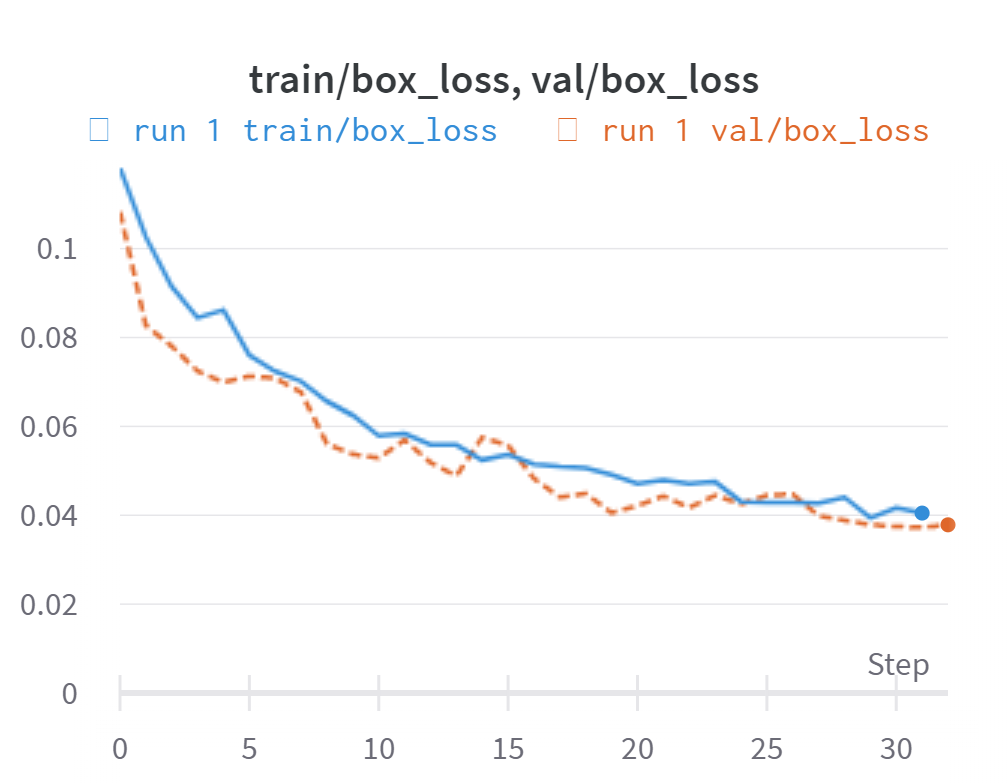
\includegraphics[width=3in]{images/05Testing/run01/Section-2-Panel-5-m94dwffr9}}
\caption{Metrics for Model 1}
\end{figure}

\begin{figure}[h!]
\subfloat{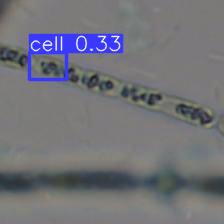
\includegraphics[width=3in]{images/05Testing/run01/easy}}
\subfloat{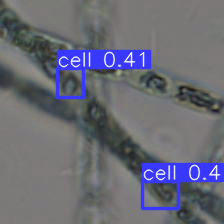
\includegraphics[width=3in]{images/05Testing/run01/hard}}
\caption{Predictions on 'easy' (left) and 'hard' (right) images from the test set by Model 1}
\end{figure}

\subsection{Model 2}

\begin{figure}[h!]
\subfloat{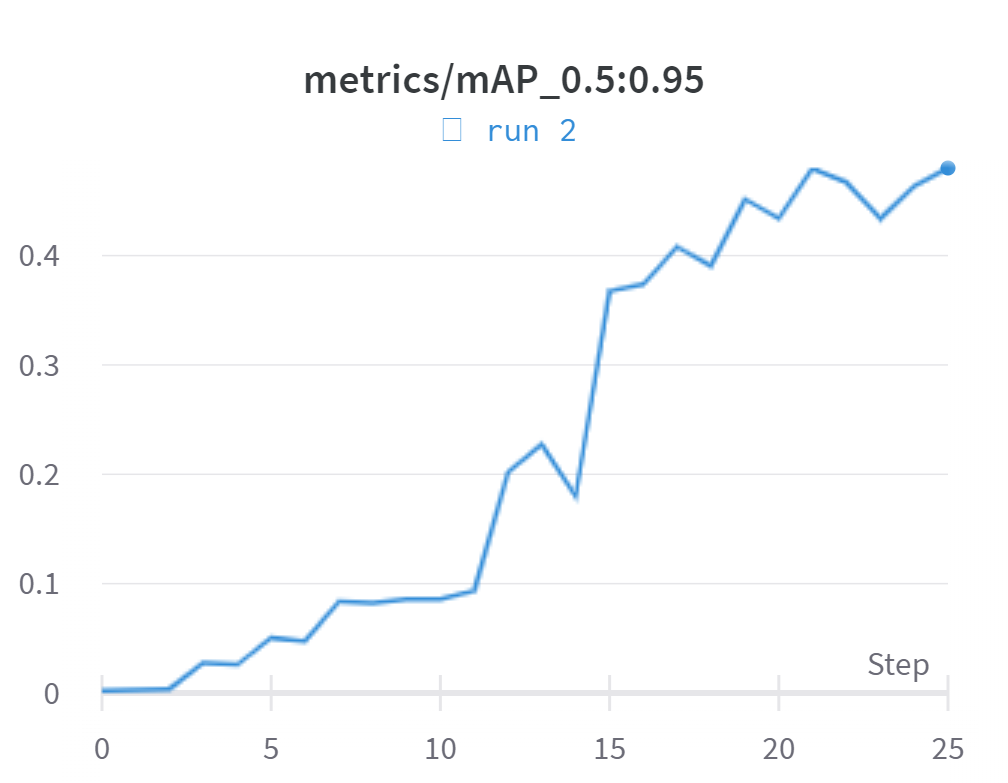
\includegraphics[width=3in]{images/05Testing/run02/Section-2-Panel-0-l24a15v4n}}
\subfloat{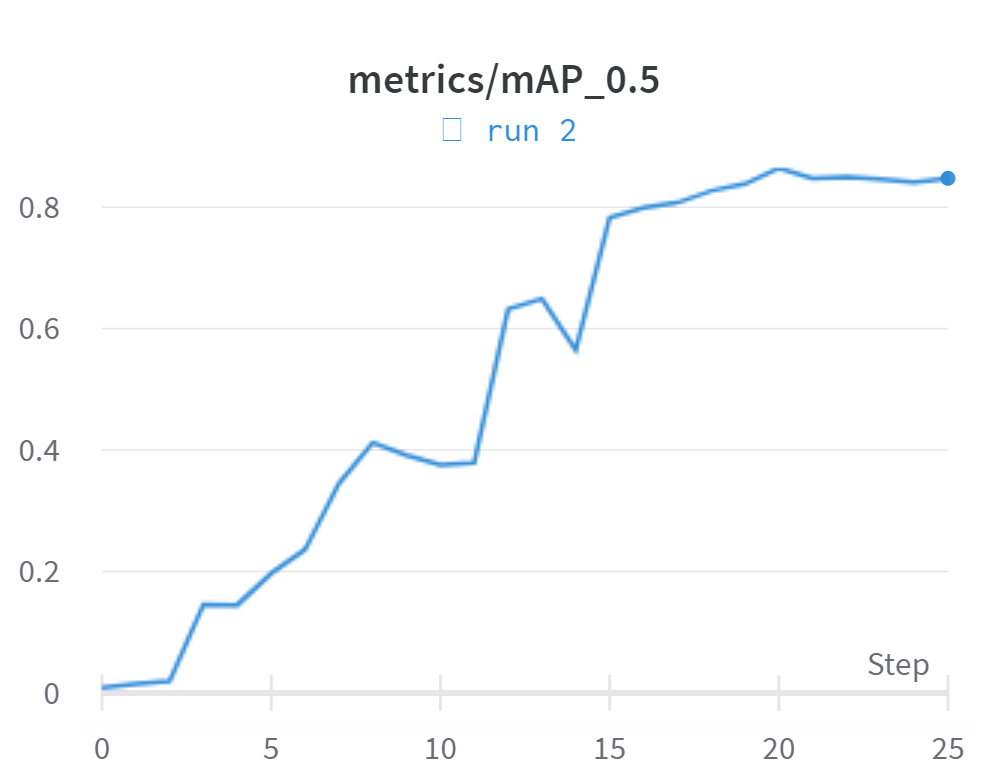
\includegraphics[width=3in]{images/05Testing/run02/Section-2-Panel-1-xq6pmkk16}}\\
\subfloat{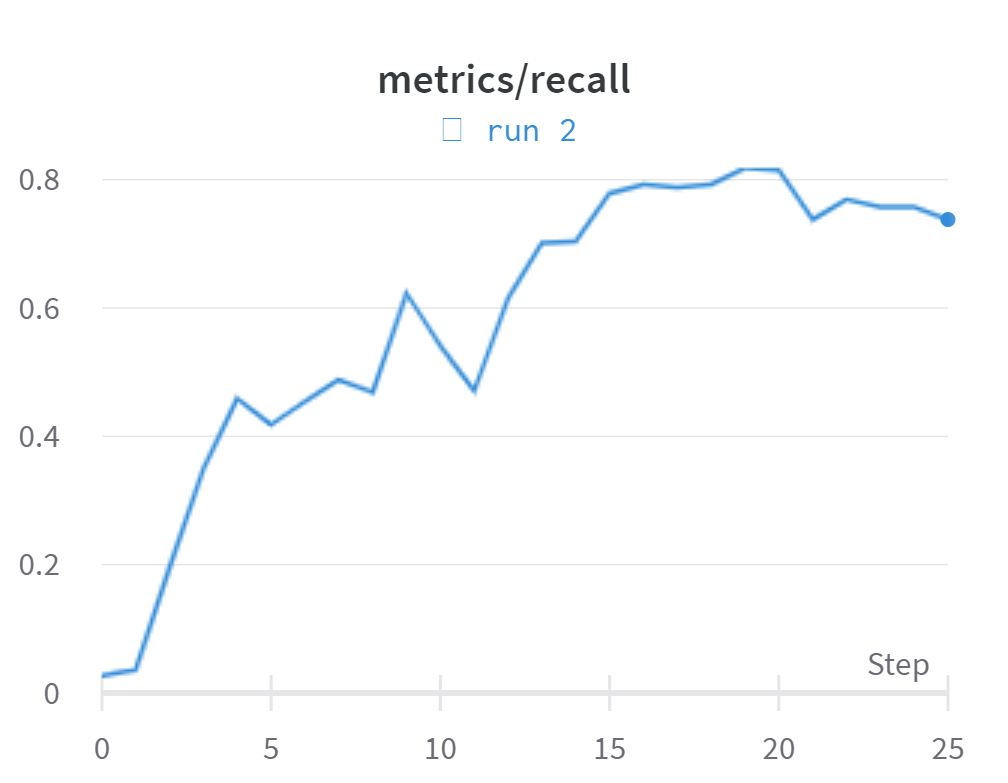
\includegraphics[width=3in]{images/05Testing/run02/Section-2-Panel-2-45rd7tgay}}
\subfloat{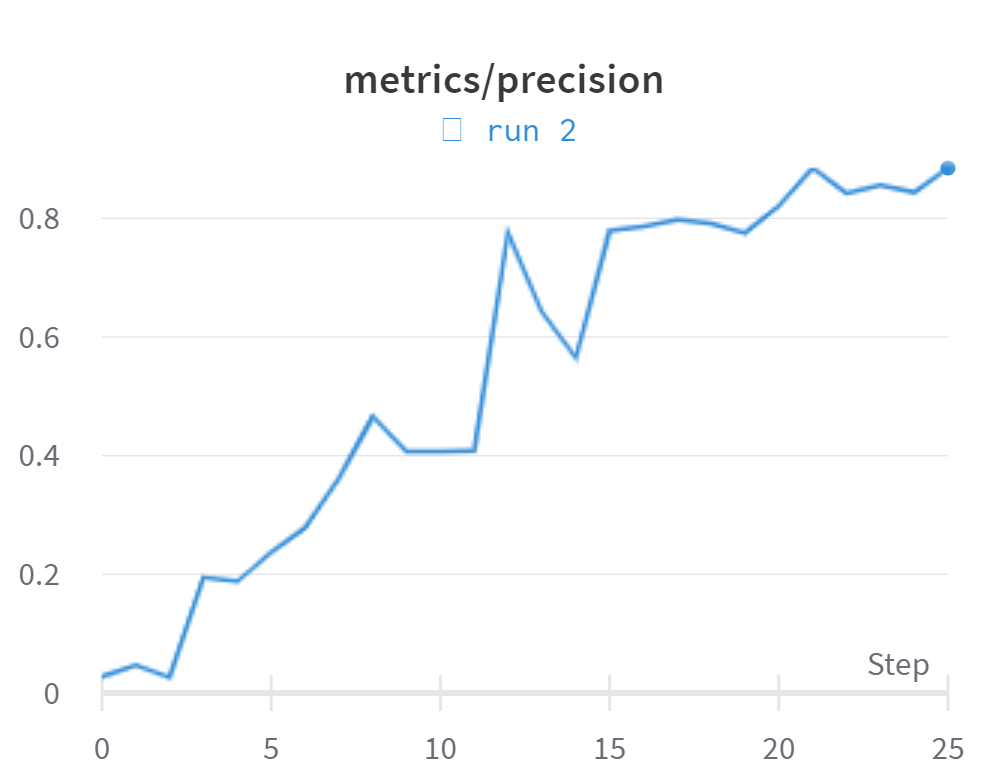
\includegraphics[width=3in]{images/05Testing/run02/Section-2-Panel-3-jsgjesr4f}}\\
\subfloat{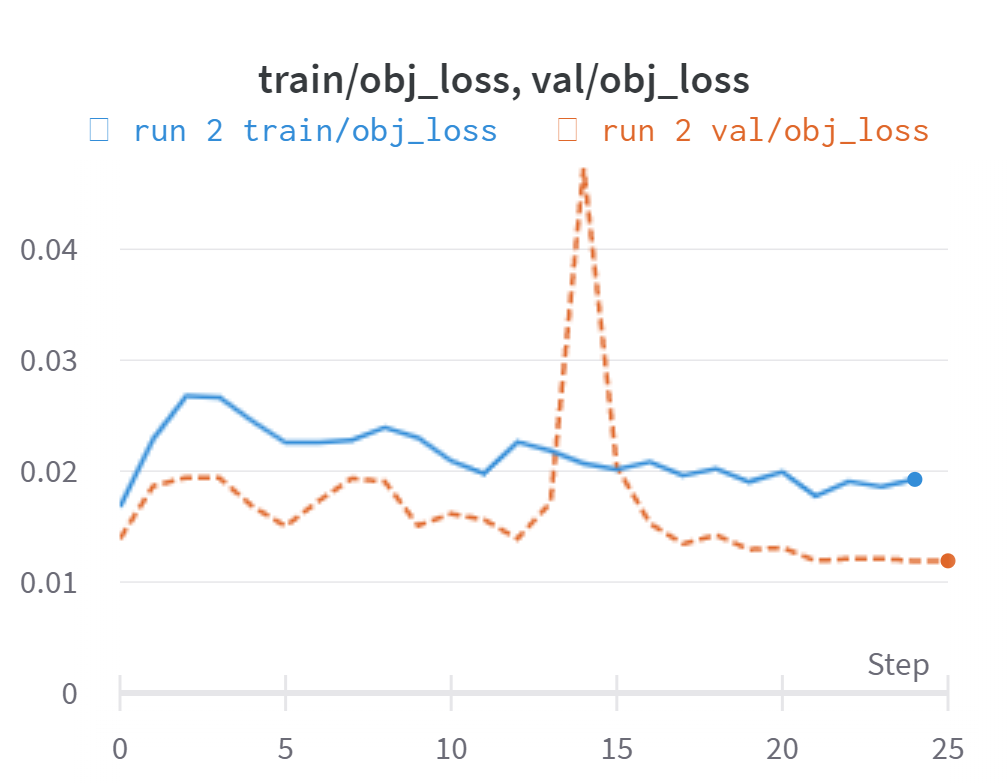
\includegraphics[width=3in]{images/05Testing/run02/Section-2-Panel-4-jgehu72sd}}
\subfloat{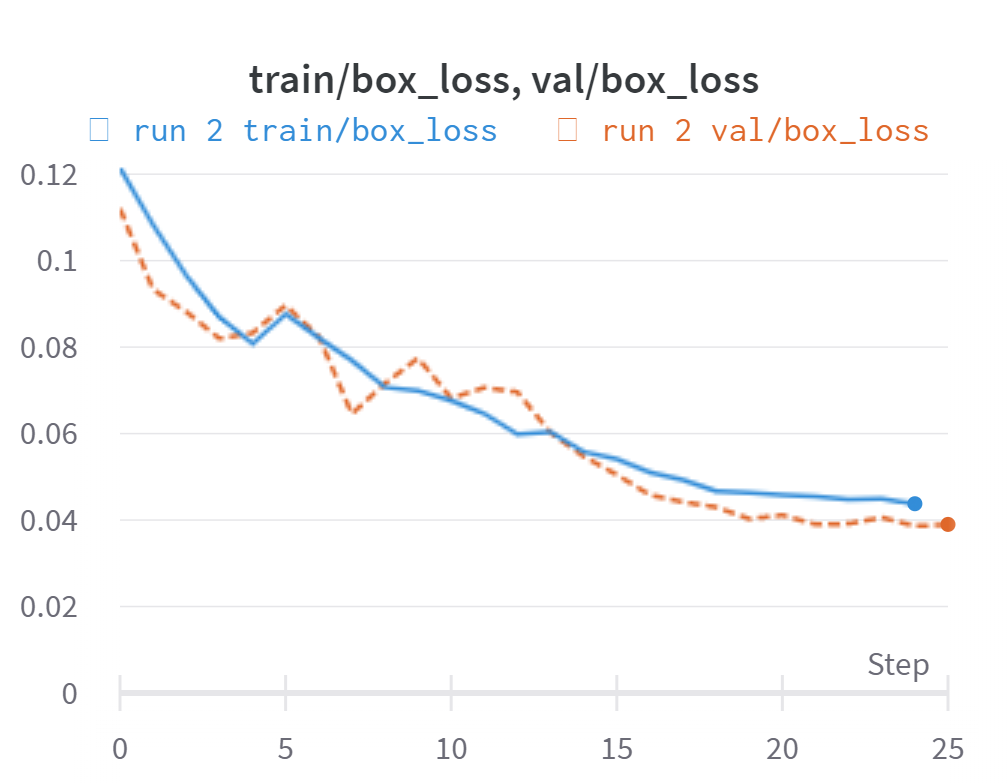
\includegraphics[width=3in]{images/05Testing/run02/Section-2-Panel-5-m94dwffr9}}
\caption{Metrics for Model 2}
\end{figure}

\begin{table}[h!]
\centering
\begin{tabular}{||c c c c c||} 
\hline
Image &  Ground Truth &  Model Count &  Num. Error &    \% Error \\
\hline\hline
37 &            81 &          193 &         112 &  138.271605 \\
39 &            58 &          100 &          42 &   72.413793 \\
41 &            86 &          147 &          61 &   70.930233 \\
44 &           102 &          235 &         133 &  130.392157 \\
\hline
\end{tabular}
\caption{Counts \& errors for Model 2}
\label{count_2}
\end{table}

\subsection{Model 3}

\begin{figure}[h!]
\subfloat{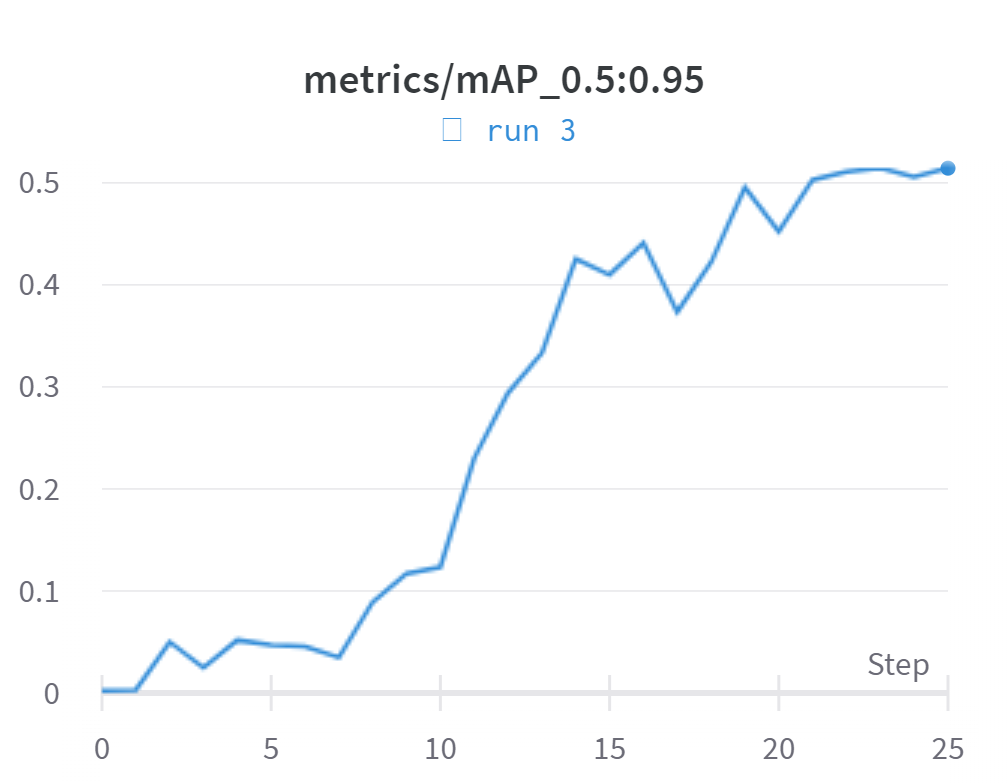
\includegraphics[width=3in]{images/05Testing/run03/Section-2-Panel-0-l24a15v4n}}
\subfloat{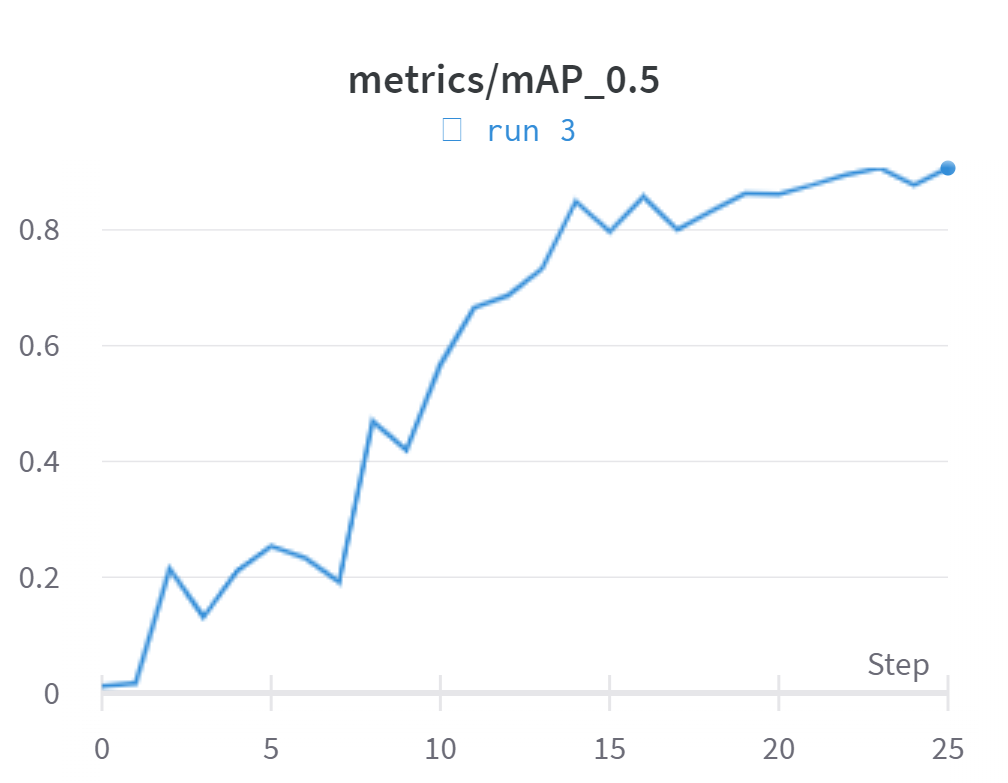
\includegraphics[width=3in]{images/05Testing/run03/Section-2-Panel-1-xq6pmkk16}}\\
\subfloat{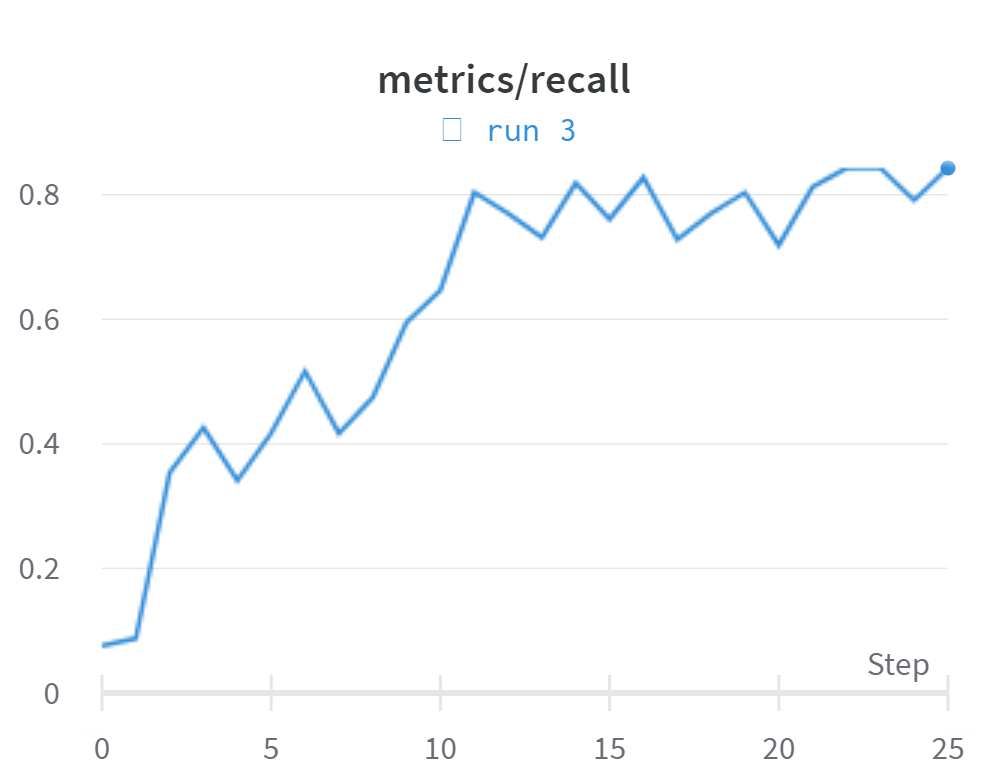
\includegraphics[width=3in]{images/05Testing/run03/Section-2-Panel-2-45rd7tgay}}
\subfloat{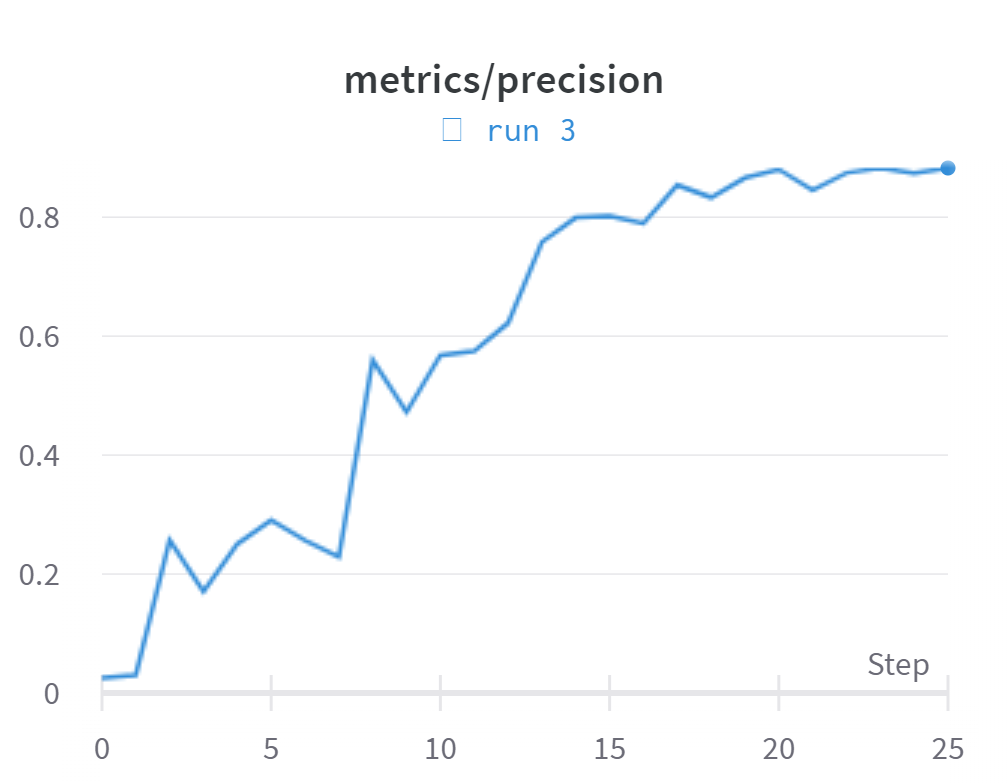
\includegraphics[width=3in]{images/05Testing/run03/Section-2-Panel-3-jsgjesr4f}}\\
\subfloat{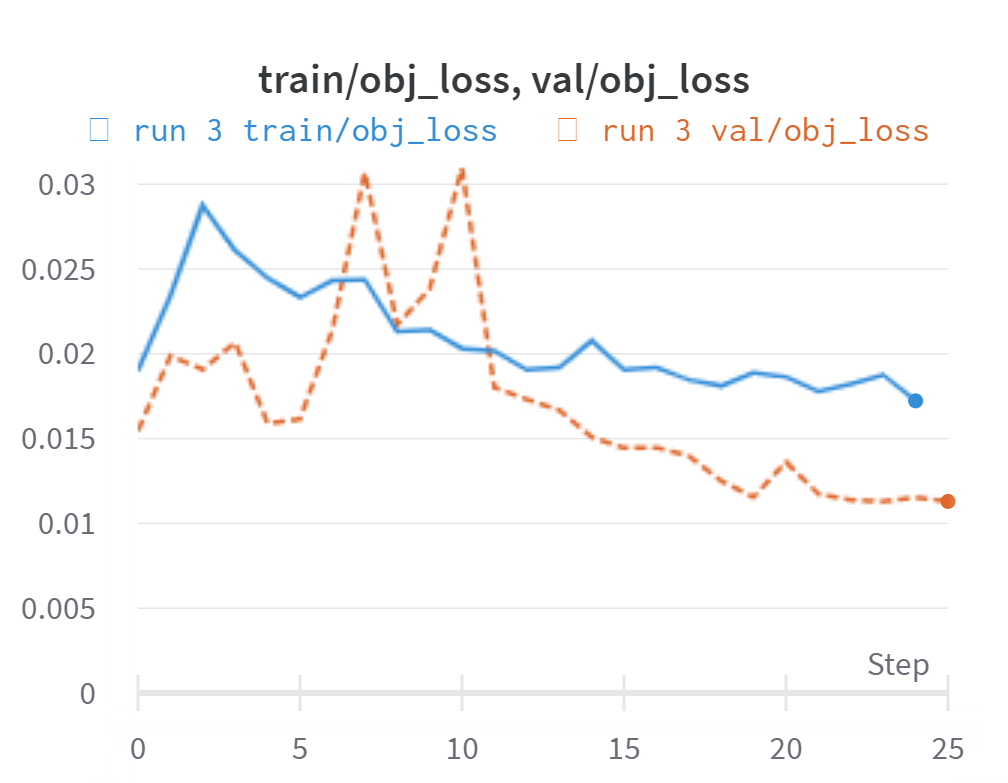
\includegraphics[width=3in]{images/05Testing/run03/Section-2-Panel-4-jgehu72sd}}
\subfloat{\includegraphics[width=3in]{images/05Testing/run03/Section-2-Panel-5-m94dwffr9}}
\caption{Metrics for Model 3}
\end{figure}

\begin{table}[h!]
\centering
\begin{tabular}{||c c c c c||} 
\hline
Image &  Ground Truth &  Model Count &  Num. Error &    \% Error \\
\hline\hline
37 &            81 &          183 &         102 &  125.925926 \\
39 &            58 &          117 &          59 &  101.724138 \\
41 &            86 &          147 &          61 &   70.930233 \\
44 &           102 &          213 &         111 &  108.823529 \\
\hline
\end{tabular}
\caption{Counts \& errors for Model 3}
\label{count_3}
\end{table}

\subsection{Model 4}

\begin{figure}[h!]
\subfloat{\includegraphics[width=3in]{images/05Testing/run04/Section-2-Panel-0-l24a15v4n}}
\subfloat{\includegraphics[width=3in]{images/05Testing/run04/Section-2-Panel-1-xq6pmkk16}}\\
\subfloat{\includegraphics[width=3in]{images/05Testing/run04/Section-2-Panel-2-45rd7tgay}}
\subfloat{\includegraphics[width=3in]{images/05Testing/run04/Section-2-Panel-3-jsgjesr4f}}\\
\subfloat{\includegraphics[width=3in]{images/05Testing/run04/Section-2-Panel-4-jgehu72sd}}
\subfloat{\includegraphics[width=3in]{images/05Testing/run04/Section-2-Panel-5-m94dwffr9}}
\caption{Metrics for Model 4}
\end{figure}

\begin{table}[h!]
\centering
\begin{tabular}{||c c c c c||} 
\hline
Image &  Ground Truth &  Model Count &  Num. Error &    \% Error \\
\hline\hline
37 &            81 &          145 &          64 &  79.012346 \\
39 &            58 &           97 &          39 &  67.241379 \\
41 &            86 &          136 &          50 &  58.139535 \\
44 &           102 &          201 &          99 &  97.058824 \\
\hline
\end{tabular}
\caption{Counts \& errors for Model 4}
\label{count_4}
\end{table}

\subsection{Model 5}

\begin{figure}[h!]
\subfloat{\includegraphics[width=3in]{images/05Testing/run05/Section-2-Panel-0-l24a15v4n}}
\subfloat{\includegraphics[width=3in]{images/05Testing/run05/Section-2-Panel-1-xq6pmkk16}}\\
\subfloat{\includegraphics[width=3in]{images/05Testing/run05/Section-2-Panel-2-45rd7tgay}}
\subfloat{\includegraphics[width=3in]{images/05Testing/run05/Section-2-Panel-3-jsgjesr4f}}\\
\subfloat{\includegraphics[width=3in]{images/05Testing/run05/Section-2-Panel-4-jgehu72sd}}
\subfloat{\includegraphics[width=3in]{images/05Testing/run05/Section-2-Panel-5-m94dwffr9}}
\caption{Metrics for Model 5}
\end{figure}

\begin{table}[h!]
\centering
\begin{tabular}{||c c c c c||} 
\hline
Image &  Ground Truth &  Model Count &  Num. Error &    \% Error \\
\hline\hline
37 &            81 &          159 &          78 &  96.296296 \\
39 &            58 &          106 &          48 &  82.758621 \\
41 &            86 &          128 &          42 &  48.837209 \\
44 &           102 &          184 &          82 &  80.392157 \\
\hline
\end{tabular}
\caption{Counts \& errors for Model 5}
\label{count_5}
\end{table}

\subsection{Model 6}

\begin{figure}[h!]
\subfloat{\includegraphics[width=3in]{images/05Testing/run06/Section-2-Panel-0-l24a15v4n}}
\subfloat{\includegraphics[width=3in]{images/05Testing/run06/Section-2-Panel-1-xq6pmkk16}}\\
\subfloat{\includegraphics[width=3in]{images/05Testing/run06/Section-2-Panel-2-45rd7tgay}}
\subfloat{\includegraphics[width=3in]{images/05Testing/run06/Section-2-Panel-3-jsgjesr4f}}\\
\subfloat{\includegraphics[width=3in]{images/05Testing/run06/Section-2-Panel-4-jgehu72sd}}
\subfloat{\includegraphics[width=3in]{images/05Testing/run06/Section-2-Panel-5-m94dwffr9}}
\caption{Metrics for Model 6}
\end{figure}

\begin{table}[h!]
\centering
\begin{tabular}{||c c c c c||} 
\hline
Image &  Ground Truth &  Model Count &  Num. Error &    \% Error \\
\hline\hline
37 &            81 &          117 &          36 &  44.444444 \\
39 &            58 &           45 &          13 &  22.413793 \\
41 &            86 &           75 &          11 &  12.790698 \\
44 &           102 &          106 &           4 &   3.921569 \\
\hline
\end{tabular}
\caption{Counts \& errors for Model 6}
\label{count_6}
\end{table}

\subsection{Model 7}

\begin{figure}[h!]
\subfloat{\includegraphics[width=3in]{images/05Testing/run07/Section-1-Panel-0-l24a15v4n}}
\subfloat{\includegraphics[width=3in]{images/05Testing/run07/Section-1-Panel-1-xq6pmkk16}}\\
\subfloat{\includegraphics[width=3in]{images/05Testing/run07/Section-1-Panel-2-45rd7tgay}}
\subfloat{\includegraphics[width=3in]{images/05Testing/run07/Section-1-Panel-3-jsgjesr4f}}\\
\subfloat{\includegraphics[width=3in]{images/05Testing/run07/Section-1-Panel-4-jgehu72sd}}
\subfloat{\includegraphics[width=3in]{images/05Testing/run07/Section-1-Panel-5-m94dwffr9}}
\caption{Metrics for Model 7}
\end{figure}

\begin{table}[h!]
\centering
\begin{tabular}{||c c c c c||} 
\hline
Image &  Ground Truth &  Model Count &  Num. Error &    \% Error \\
\hline\hline
37 &            81 &           95 &          14 &  17.283951 \\
39 &            58 &           46 &          12 &  20.689655 \\
41 &            86 &           95 &           9 &  10.465116 \\
44 &           102 &          127 &          25 &  24.509804 \\
\hline
\end{tabular}
\caption{Counts \& errors for Model 7}
\label{count_7}
\end{table}

\section{Source Code}
Source code is hosted on GitHub and can be accessed at \url{https://github.com/adamindeen/CM4105-Honours}.

\section{Project Log}
The project log can be found in the project's Git repository under the filename \verb`log.md`.\\

\paragraph{23/09/2021}
1-hour meeting. Discussed the current method under investigation:\\
1. take input image, turn it into patches
2. use trained GAN to do style transfer on the patches
3. Process ground truth to get the cell markings \verb`validation_steps`
4. reassemble the patches and count the cells.

Received reading pointers:\\
   - GANs and Neural Style Transfer (as a specific application, transformation of horses into zebras with CGANs)
   - ImageJ
   - Yolo

Submitted template matching as a possible alternative solution.

\paragraph{30/09/2021}
No meeting. Continued with reading.

\paragraph{07/10/2021}
Meeting to clarify the project proposal. Project options discussed:\\
- Implement a GAN (such as pix2pix) for style transfer of micrographs into computer-interpretable 'binary' images
- Implement a model to count 'cells' in 'binary' images
- Implement a web interface for an existing model\\

It was clarified that the existing solution is still under development and there is still significant scope for refinement.

\paragraph{08/10/2021}
Completed & submitted Project Proposal & Ethics Form. Project is to implement a machine learning model for cell counting, not a web interface for such a model.\\

Feedback on Project Proposal:\\
- Citations: the link is fine in the proposal but make sure you cite properly in the actual project document. Use Harvard if you can, but if you're using LaTeX, Vancouver might be easier (it's hard to find a decent Harvard LaTeX bib style)
- You're missing the term "semantic segmentation". That's what the "binary" file is - grey for background, black for trichome, white for cell-centre. Semantic segmentation provides a mask showing the "meaning" of each pixel (i.e. which object it belongs to).
- You're missing "evaluation of my technique" in your milestones list. I know it'll probably be an iterative approach (develop method, how good is it? Make it better. How good is it now?), but you can mention evaluation of your own model as one of your objectives. AND you can then say that evaluating such a model is a key technique (how do you know your model is any good?).
- If you wanted to expand your project plan, you might take a "months and milestones" approach, and you start doing that by looking at your deadlines for the honours project. This will be more important later when you might have to pull yourself out of a research rabbit-hole to make sure you complete the project on time (even if it's not "complete" to the standard you want!).\\

Clarification on ethics: the dataset of micrographs is internal to the University and does not create any data protection concerns.

\paragraph{14/10/2021}
1-hour meeting post-Project Proposal submission. Discussed:\\
- Labelme
- Grabcut to process rough binary map produced by high pass filter
- Object detection & region proposal in YOLOv5\\

A possible specification of a project within the bounds of the proposal was suggested: retraining YOLOv5 to detect, localise, and count cyanobacteria cells.

\paragraph{27/10/2021}
Feedback received for Project Proposal:\\

The project proposal is very thorough and clear. There are a couple of places where I think you could improve. You mention research participants, but that doesn’t necessarily fit in with the rest of the proposal (any more), and you’ve named some key techniques but you could do with slightly more detail on some of them. For example, machine learning can be implemented in many ways, and python libraries like keras or pytorch facilitate this. Your project plan is detailed enough that it will see you complete the project in a timely manner, and the background and motivation sections are excellent. Your writing style is lucid and appropriate for the task.

\paragraph{04/11/2021}
No meeting. Continued with reading.

\paragraph{12/11/2021}
Decided to postpone meeting in favour of continuing with Literature Review.

\paragraph{15/11/2021}
In-person meeting discussing the literature review:\\
- Follow a 'here's how it was done, here's why it was good, here's how it relates to my  project' approach
- The example literature reviews represent exactly what is required
- Include abstract & table of contents
- Include *applied* references, i.e. those which can be 'tied back' to the project requirements. For example, YOLO has implementations in both Keras and Pytorch. This is a piece of info worth tying back to the project's non-functional requirements. Another could be a comparison of regularisation functions Adam and SGD

\paragraph{18/01/2022}
30-minute in-person meeting. Revisited the project scope (retrain YOLO on Micropics, repeat if possible) and the state of the project so far (no news).

\paragraph{24/01/2022}
Began familiarisation with YOLO & micropics repo.

\paragraph{25/01/2022}
Began critical appraisal of image annotation tools (Labelstudio vs Labelme).\\
Meeting discussed:
- The process of patching images (if blank patches are to be removed, a new approach will need to be developed since the existing one presumes a processed image with a black background)
- The structure of the final report (Design, Implementation, Evaluation)

\paragraph{01/02/2022}
Meeting
What metrics does YOLO output after training? Keep in mind that an IOU of 20\% is good\\

Report
Structure should include ‘Design’ and ‘Results’ sections
Including a GitHub link might influence professionalism grade
Add more requirements or refine existing ones (the 
Evaluate yolo & other tools
Demonstrate whether it’s a good idea to 
Include paragraph on density estimation, explain why it is likely to be unsuitable (highly varying density of cells across image). Justify YOLO
Have you built the code correctly? Have you built the correct code?\\

Have you tested the hypothesis that giving it more data yields better results
Write a script that removes suffixes from images output by Label Studio
What was a 
Ethics - cover them all
Assume reader will only read the opening and closing\\

Match opening \& closing paragraphs of section
FRACTAL
Write like JSON
Describe graphs
Shamal isn’t a deep learning guy\\

Use the page limit even if you’re repeating yourself
Good comeback for ‘I would like to see more on this\\

If I just read the section titles/ start \& end of each section I should get it
State the obvious\\

3-5 references for poster
No page sums in refs\\

Main meat of the demo is showing the code/explaining the results


\paragraph{23/02/2022}
In-person meeting. Discussed:
- HOG descriptors
- Transfer learning as the basis for retraining YOLO
  - Justify the model used as a basis
- Reducing oscillation (reduce learning rate by factor of 10 or 100)
- The possibility of data processing introducing bias
- Distortion/occlusion/foreshortening of images
- Writing up
  - Write in the order things are done
  - Methodology, Results, and Evaluation are graded separately
  - Read the grading grid
  - Reflection - justify the method used
  - The first and last paragraph of a section, apart from the rest, should make sense
  - If it doesn't correspond to an Aim/Objective, it doesn't count
  - Refer to As\&Os in Conclusion
  
\paragraph{26/02/2022}
Set up DGX \& became familiarised with the system.

\paragraph{15/03/2022}
15-minute Teams meeting. Further discussed DGX setup.

\paragraph{22/03/2022}
Brief in-person discussion:

- Development can continue for the project duration and concurrently with the writeup

\paragraph{24/03/2022}
Email check-in:

- '...Record absolutely everything (screenshots, accuracy etc. etc.). If the conclusion of your project is just “We need to label way more than just 20 images to get good results because the accuracy is pretty terrible with just a few labelled images”, then that is probably a valid conclusion, but make sure you are recording the data as you go so you don’t “lose” any experiments in the write up. Write up absolutely everything you have, whether it works or not.'
- '...I’m planning on taking leave 4-8 April inclusive, but if you desperately need me, I will be checking email infrequently.'

\paragraph{13/04/2022}
Entire 20-image dataset labelled (first pass).

\paragraph{14/04/2022}
Unsuccessfully attempted to set up a DGX Jupyter notebook to run inference.

\paragraph{15/04/2022}
1-hour meeting. Mainly tried to resolve the aforementioned DGX issue without success (another user appears to be occupying all the GPUs). It was decided Google Colab should be used instead while the issue is investigated.

\paragraph{16/04/2022}
Began structuring report according to RGU LaTeX template. Purchased Colab Pro subscription for GPU training.

\paragraph{17/04/2022}
Test run using GPU runtime. Good results.

\paragraph{18/04/2022}
Labelled dataset (2nd run), including partially visible and out-of-focus cells, followed by 2nd run of training. Moved one image each from the validation and test sets to the training set for a 70/30 train/test split, followed by 3rd run of training.

\paragraph{19/04/2022}
4th run of training (increased epochs to 50), with improved results (based on metrics). Updated Jupyter notebook to include script to sum counts for all patches (for each image in the test set).

\paragraph{20/04/2022}
Created spreadsheet to capture model counts vs ground truth counts and determine error (absolute & percentage). Discovered discrepancy between counting performance & metrics (model counts are 2-3x ground truth). 30-minute remote meeting on poster deliverable and report:

- Increasing the training data increased performance (so more labelled data would be good)
- Increasing the labels increased performance (but also increased false positives?)
- Increasing the training time (number of steps?) improved performance (in terms of mAP and count?)
- The problem might not be in missed detection, but rather in false positives
- Does better mAP correlate with better cell count?
- An alternative analysis might calculate error for each patch and then average across the image
- Emphasise the fact that since a base YOLO model would be unsuitable, it was retrained 4 times, showing a development process
- The dataset is not perfect - only 1 expert annotator
- Mention the selection of YOLOv5 model in Design - speed? Portability?

Submitted. 

\paragraph{21/04/2022}
Continued with writeup. Added Requirements Specification and section on labelling tools to Methodology

\paragraph{22/04/2022}
Development:
- General cleanup of Colab notebook
- Added evaluation section with DataFrame
- Trained model based on YOLOv5l

Report:
- Made progress in Design
- Started Implementation

\paragraph{23/04/2022}
Contacted school office to arrange degree show session. 

Report:
- Made substantial progress in Design \& Implementation chapters
- Added project proposal \& ethics form to appendix

\paragraph{24/04/2022}
Report:
- Made some progress in Design

\paragraph{25/04/2022}
Trained models 6 \& 7 based on YOLOv5l, with excellent results.

Report:
- Added poster to appendix
- Made substantial progress in Testing

\paragraph{26/04/2022}
Submitted incomplete draft of the final report for feedback. Discussed the report deliverable as a whole in the final meeting (fractal writing, reference to figures within the text, proofreading)

\paragraph{27/04/2022}
Degree show. Presentation to supervisor & second marker was mostly successful with some lessons learned (future work must be clarified)

\paragraph{28/04/2022}
Feedback received for initial draft. All implemented.

\paragraph{29/05 - 06/05/2022}
Continued work on final report.

\includepdf[scale=0.9, pages=1, pagecommand=\section{Project Proposal}]{docs/proposal.pdf}
\includepdf[scale=0.9, pages=2-]{docs/proposal.pdf}

\includepdf[scale=0.9, pages=1, pagecommand=\section{Ethics Form}]{docs/ethics.pdf}
\includepdf[scale=0.9, pages=2-]{docs/ethics.pdf}

\includepdf[scale=0.8, pages=1, pagecommand=\section{Degree Show Poster}]{docs/poster.pdf}

\end{appendices}



\end{document}